\documentclass[12pt,letter]{article}
\usepackage[DIV=14,BCOR=2mm,headinclude=true,footinclude=false]{typearea}
\renewcommand{\baselinestretch}{1.5} 
\usepackage{latexsym}
\usepackage{amsmath}

\usepackage{titlesec}
%\titleformat{\section}[block]{\color{blue}\Large\bfseries\filcenter}{}{1em}{}
%\titleformat{\subsection}[hang]{\bfseries}{}{1em}{}

%\usepackage{sectsty}
%\sectionfont{\centering}

\usepackage{pdflscape}

%\usepackage{MinionPro}
\usepackage{amssymb}

\usepackage{hyperref}
\usepackage{tikz}
\usepackage{verbatim}
\usepackage{natbib}
\usepackage{color, colortbl}
\usepackage{appendix}
\usepackage{amsmath,amsthm}

%\usepackage[]{figcaps}

\usepackage{wasysym}


\newcommand{\Rho}{\mathrm{R}}
\newcommand{\Kappa}{\mathcal{C}}
\newcommand{\Omicron}{\mathcal{O}}
\newcommand\omicron{o}
\newcommand{\Tau}{\mathrm{T}}

\usetikzlibrary{arrows,shapes}

\definecolor{Gray}{gray}{0.9}

\newtheorem{result}{Result}
\newtheorem{theorem}{Theorem}
\newtheorem*{theorem*}{Theorem}
\newtheorem{conjecture}{Conjecture}[section]
\newtheorem{corollary}{Corollary}[section]
\newtheorem{lemma}{Lemma}[section]
\newtheorem*{lemma*}{Lemma}
\newtheorem{proposition}{Proposition}[section]
\newtheorem{definition}{Definition}[section]
\newtheorem{assumption}{Assumption}[section]


\theoremstyle{definition}
\newtheorem{example}{Example}

\theoremstyle{remark}
\newtheorem*{remark}{Remark}

\theoremstyle{claim}
\newtheorem{claim}{Claim}

%\usepackage{chngcntr}
%\counterwithin{figure}{section}


\pgfdeclarelayer{background}
\pgfsetlayers{background,main}

\tikzstyle{vertex}=[circle, draw
%,fill=black!25
,minimum size=12pt
,inner sep=0pt
]
\usetikzlibrary{decorations.pathreplacing}
\tikzstyle{selected vertex} = [vertex, fill=red!24]
%\tikzstyle{unknown vertex} = [vertex, fill=black!25]
\tikzstyle{unknown vertex} = [vertex, fill=white]
\tikzstyle{edge} = [draw,thick,-]
\tikzstyle{weight} = [font=\small]
\tikzstyle{selected edge} = [draw,line width=5pt,-,red!50]
\tikzstyle{ignored edge} = [draw,line width=5pt,-,black!20]
\newcommand{\bigtimes}{\mathbin{\tikz [x=1.4ex,y=1.4ex,line width=.2ex] \draw (0,0) -- (1,1) (0,1) -- (1,0);}}%


%\linespread{1.5}

\begin{document}
%\fontsize{12}{20pt}\selectfont

\title {Coordination in Social Networks: Communication by Actions}
\author {Chun-Ting Chen}
\date{\textit{draft: v4.0}}
\maketitle

\begin{abstract}

%This paper studies a collective action problem in a setting of discounted repeated coordination games in which players know their neighbors'  inclination to participate as well as monitor their neighbors' past actions. I define \textit{strong connectedness} to characterize those states in which, for every two players who incline to participate, there is a path consisting of players with the same inclination to connect them.  Given that the networks are fixed, finite, connected, commonly known, undirected and without cycles, I show that if the priors have full support on the strong connectedness states, there is a (weak) sequential equilibrium in which the ex-post efficient outcome repeats after a finite time $T$ in the path when discount factor is sufficiently high. This equilibrium is constructive and does not depend on public or private signals other than players' actions.




\end{abstract}


\section{Introduction} 

%This paper studies collective actions in a setting of discounted repeated coordination games, where information and monitoring structures are modeled as networks. Players are uncertain about the states of nature but can observe their neighbors' actions. I would like to explore what kinds of networks can induce players to solve the underlying uncertainty in order to coordinate with the ex-post efficient outcome. Though the motive of this study is to understand the dynamic of social movements, a general interest centers on the collective action behaviors within social structures.
%
%Consider pro-democracy movements. Strong discontents overthrowing a regime may exist, but it is difficult to organized around these discontents because information about the existence of such discontents is not always transparent. For instance, in East Germany, the government had control over the electoral system and the mass media, and the eavesdropping by secret agents had impeded people from showing their discontents. As \citep{Karl-Dieter1993} or \citep{Chwe2000} have suggested, such discontents may be revealed only to someone whom you trust or have an intimate relationship with, but are hardly revealed publicly. This lack of common knowledge about the existence of strong discontent may impede people from conducting a one-shot uprising due to the fear of possible failure (e.g., \citep{Chwe2000} in proposing a static model to characterize the networks that provide common knowledge about peoples' discontents). However, an event may trigger a later event (e.g., \citep{Lohmann2011} in using informational cascade model to explain consecutive demonstrations in East Germany 1989-1991). When rebels are aware of the scale to transmit relevant information about the level of collective discontent through their actions, they might be willing to act although it might be at risk of facing failure. I view such risky actions as a part of an equilibrium strategy and the entire movement as a learning process. 
%
%
%
%
%Inspired by \citep{Chwe2000}, I model such dynamic collective action in the following way. Players repeatedly play a $k$-\textit{Threshold game} with a parameter $k$ in a network. There are two types of players located in the network, one we called them \textit{Rebel} and one we called them \textit{Inert}.  Players' types and their actions can be observed only by their neighbors. A Rebel has two actions, which are \textbf{revolt} or \textbf{stay} while an Inert has only one action, which is \textbf{stay}. A Rebel will get payoff as $1$ if he chooses \textbf{revolt} and more than $k$ players choose \textbf{revolt}; he will get payoff as $-1$ if he chooses \textbf{revolt} and less than $k$ players choose \textbf{revolt}; he will get payoff as $0$ if he chooses \textbf{stay}. An Inert will get payoff as $1$ if he chooses \textbf{stay}.
%
%Since a Rebel may not know how many Rebels exist in this world, Rebels' payoff structure captures the idea that \textbf{stay} is a safe arm and \textbf{revolt} is a risky arm. Given a common prior $\pi$ over players' types, players play this $k$-Threshold game infinitely repeatedly with a common discount factor $\delta$. Cheap talk is not allowed, no outside mechanism serves as an information sharing device. 
%
%Rebels then communicate with each other by playing actions. For different $k$ and different network structures, I am looking for a sequential equilibrium which has the property of \textit{approaching ex-post efficient} (\textit{APEX} henceforth) to investigate the information sharing behavior in the networks. An equilibrium is APEX if and only if {the tails of actions in the equilibrium path repeats the static ex-post efficient outcome after a finite time $T$}.  This refinement serves to check if players have already learned the relevant information in the equilibrium path. If there are at least $k$ Rebels in this society, then \textit{all} Rebels should \textbf{revolt} after $T$ as if they have known that more than $k$ Rebels exist; otherwise, \textit{all} Rebels should \textbf{stay} after $T$. The Rebels' incentives to communicate are affected by their positions in networks since networks are structuring the information and monitoring structure.
%
%In order to get a quick intuition about Rebel's learning process in the proposed framework, consider the $k$-Threshold game with $k=n$ and assume that payoff is hidden. When $k=n$, a Rebel can get positive payoff only if all the players are Rebels. Given that the networks are fixed, finite, connected, commonly known, and undirected (\textit{networks} henceforth), an APEX sequential equilibrium can be constructed by a contagion-like argument. This argument is to treat \textbf{stay} as the message of ``there is an Inert out there''; and treat \textbf{revolt} as the message of ``there could be no Inert out there ''. If a Rebel has an Inert neighbor, then he plays \textbf{stay} forever. If he has no Inert neighbors, then he plays \textbf{revolt} until he observes that some of his neighbors play \textbf{stay}, and then he shifts to play \textbf{stay} forever. Since the networks are finite,  within finite periods, a Rebel will learn that there is an Inert out there if some neighbors have played \textbf{stay} and learn that there is no an Inert out there otherwise.
%
%The non-trivial cases appear when $k<n$. The $k=n$ case is easier because the underlying relevant information is to tell ``Is there an Inert out there?''. I can construct equilibrium when $k=n$ by using single-period binary actions, $\{\textbf{stay},\textbf{revolt}\}$, to separate the states into two parts, ``no Inerts'' or ``some Inerts''. In other words, these single-period actions can generate distinguishable distribution of signals to inform players in telling the true states of nature.\footnote{e.g., \citep{Fudenberg2010} or \citep{Fudenberg2011}.} 
%However, when $k<n$, the relevant information is to tell ``Are there at least $k$ Rebels out there?'', and thus these binary actions have to carry more information to reveal the states. As I will show later, several sequences of actions will be used to transmit Rebels' private informations and to control Rebels' beliefs in equilibrium. In the equilibrium path, two kinds of sequence will be used. The first kind, \textit{reporting messages}, is to report their private information about the states of nature; the second one, \textit{coordination messages}, is to inform Rebels about whether some other Rebels have known the relevant information.  Specifically, in the equilibrium path, Rebels will play the coordination message to inform other Rebels whenever they have known the relevant information, and those other Rebels will play the same message again to inform other Rebels. The coordination message means to serve as a short-cut to track individuals' higher-order beliefs about ``Have some Rebels known the relevant information?'', ``Have some Rebels known some Rebels have known the relevant information?'', etc.
%
%
%Note that communication is costly in the sense that playing \textbf{revolt} is risky. Due to being discounting, Rebels always seek the opportunity to manipulate their messages to save their costs in the time horizontal line.\footnote{Indeed, allowing cheap talk or using limit-of-mean preference (e.g., \citep{Renault1998}) will solve this coordination problem.}
%A free-rider problem may occur when reporting information incurs costs. I give an example here to illustrate this issue. Consider a situation where two nearby Rebels share information.\footnote{C.f.~Example~\ref{ex_free_rider_tree}} 
%Suppose that these two Rebels can learn the true state after acquiring information from each other's truthful reporting. Furthermore, we suppose that each of them can freely initiate the coordination after exchanging information. In this instance, truthful reporting is not the best response because a player can wait given that the other will report truthfully. The intuition behind the above scenario is to see the future coordination as a public good. This public good can only be made by Rebels' truthful reporting, which incurs some costs.
%
%
%The main result will show that this coordination problem can be solved in the {acyclic} networks . Here, I define a \textit{path} in $G$ is a sequence consisting of nodes without repetition in which a node is a neighbor of a previous node. Then I define an undirected network acyclic $G$ by defining a network in which the path between different nodes is unique. After I define \textit{strong connectedness} as the property that there is always a path consisting of Rebels to connect any pairs of Rebels,  the main result shows:
%
%\begin{result}\textbf{(Main Result)}
%For $n$-person repeated $k$-Threshold game with parameter $1\leq k \leq n$ played in any acyclic network, if $\pi$ has full support on the strong connectedness, then, there is a $\delta^{*}$ such that a (weak) APEX sequential equilibrium exists whenever $\delta>\delta^{*}$.  
%\end{result}
%
%Here, the assumption that $\pi$ has full support on strong connectedness means that $\pi$ assigns positive probability on same states if and only if those states exhibit strong connectedness. This assumption is to make sure that the underlying game is not reduced to an incomplete information game which is without communication.  To see this, recall that an Inert always plays \textbf{stay}. Rebels cannot communicate with some Rebels by their actions if an Inert happens to separate them. For instance, in a wheel network, an incomplete game without communication is that the central player is an Inert while the peripheral players are all Rebels. It is impossible to find an APEX equilibrium in this instance unless $k=1$.
%
%The out-of-path belief serves as a grim trigger as follows. Whenever a Rebel detects a deviation, he believes that all other players outside his neighborhood are Inerts. Thus, if there are less than $k$ Rebels in his neighborhood, he will play \textbf{stay} forever. With this out-of-path belief and the constructed equilibrium strategies, the belief system satisfies \textit{updating consistency}(\citep{Perea2002}), while it may not satisfy full consistency (\citep{Krep_Wilson1982}). \footnote{Updating consistency requires that, for every player, for every player's strategies, for every information sets $s^1,s^2$ where $s^2$ follows $s^1$, if $s^2$ happens with positive probability given $s^1$ and given players' strategies contingent on $s^1$, then the belief over $s^2$ should satisfy Bayesian updating conditional on the belief over $s^1$ and players' strategies contingent on $s^1$. In other words, the updating consistency require that players hold beliefs in every information sets and hold updated beliefs that follows previous beliefs. This requirement imposes restrictions on out-of-path beliefs that induce sequential rationality, although it is weaker than full consistency in the sense that full consistency implies updating consistency.}
%
%The establishment of an equilibrium construction starts from building a communication protocol. By exploiting the assumption of finite and commonly known network, I assign each node a distinct prime number. Then I let reporting messages carry the information about the multiplication of nodes' prime numbers. Since the multiplication of prime numbers can be defactorized uniquely, the reporting messages thus carry the information about those nodes' locations in a network. Next, I let two phases, reporting period and coordination period, occur in turns in the time horizon, where the reporting (resp. coordination) messages are played in the reporting (resp. coordination) period. In the coordination period, whenever a Rebel tells the relevant information, such Rebel inform his nearby Rebels by sending coordination messages. Those nearby Rebels then continue to inform their nearby Rebels by sending coordination messages, etc. Then, after the coordination period, if a Rebel has received a coordination message, he is certain that all Rebels have commonly known that they can tell the relevant information. 
%
%I call a complete two-phases, starting from a reporting period and ending with a following coordination period, a \textit{block}.  In a block, I control the inter-temporal incentives in playing between reporting and coordination messages as follows. First, I let both of the coordination messages, one of them can initiate the coordination to \textbf{revolt} and another one can initiate the coordination to \textbf{stay}, incur no expected cost. Second, I let Rebels play \textbf{revolt} after a block only if they have observed the coordination message to \textbf{revolt} and observed some reporting messages  which incur some expected costs. However, the continuation behavior after observing the coordination message to \textbf{stay} is not contingent on any reporting message. When a Rebel looks forward future coordination to \textbf{revolt}, he may have the incentive to take a risk to influence Rebels' future behavior forwardly; otherwise, he just plays \textbf{stay}. Next, in the equilibrium path, I make sure that Rebels will play ex-post efficient outcome repeatedly right after a block if some Rebels have initiated the coordination in that block. I will argue that only those Rebels who have been able to tell the relevant information after reporting period have the incentive to initiate the coordination. This is because they do not need further evidence to prove that whether the revolution will be successful. This argument is to show that a Rebel other than them will not take advantage to send that free coordination message to initiate the coordination. This is because players cannot update further information if all their neighbors continue to play the same actions in the future. When $\delta$ is high enough, he will not initiate the coordination to impede his own learning process to achieve the ex-post efficient outcome.
%
%I then characterize Rebels' incentive in taking risks and control how much \textbf{revolt} they should play to sustain an APEX equilibrium. In the equilibrium path, a Rebel iteratively updates his relevant information given other Rebels' \textbf{revolt}-\textbf{stay} finite sequence in reporting their information about the state, and a Rebel takes risks only if his current relevant information has not been acquired by other Rebels. In the equilibrium path, a Rebel thus believes that ``more other Rebels are out there'' if and only if his nearby Rebels take risks to report their existence. Some specified forms of reporting messages are introduced, and the out-of-path belief is to enforce Rebels not to play differently from them.
%
%The key step here is to construct a special reporting message which incurs the least expected cost in taking risks, and this message should be considered as a part of the equilibrium path. I denote this special reporting message as $\langle 1 \rangle$. To see its importance, consider the concept of pivotal Rebel. Here, a pivotal Rebel is defined as the Rebel who is sure that he can know the relevant information right after a reporting period given that other Rebels will report their information truthfully. Now suppose playing $\langle 1 \rangle$ is not considered as a part of the equilibrium path, and suppose a Rebel finds himself as a pivotal Rebel during a reporting period while he has not yet reported anything in that period. It could be possible for him to find a profitable deviation by taking less risks (i.e. by playing less \textbf{revolt}), which can not be detected by at least $k$ Rebels although some Rebels can indeed detect such deviation. Since those Rebels who detected such deviation will play \textbf{stay} forever by the out-of-path belief, and this pivotal Rebel can initiate the coordination to \textbf{revolt} by convincing other Rebels to play \textbf{revolt}, the APEX fails. To solve this problem, I introduce message $\langle 1 \rangle$ to let pivotal Rebels identify themselves, while I let coordination messages to \textbf{revolt} or to \textbf{stay} have to be initiated when $\langle 1 \rangle$ has been played in the equilibrium path to prevent non-pivotal Rebels from mimicking pivotal Rebels.
%
%The major difficulties remaining to solved are the situations where there are multiple pivotal players nearby each other. In such phenomenon, the APEX may fail since playing $\langle 1 \rangle$ does not answer ``how many Rebels has a pivotal Rebel known?'' although it does address ``a pivotal Rebel exists''. The assumption of acyclic networks is crucial of solving these problems. If the networks are acyclic, I will show it later that there are only two kinds of pivotal Rebels. One kind is that they have known there are at least $k-1$ Rebels. The other kind is that they will know the true state given other Rebel neighbors' truthful reporting. I call the latter case a free-rider problem. If the networks are acyclic, Lemma~\ref{lemma_at_most_two_nodes} will show that the free-rider problems only happen between two nearby pivotal Rebels in only one block in the equilibrium path. Further, these two nearby Rebels will know that this free-rider problem will occur before the game entering into this block. The consequence of Lemma~\ref{lemma_at_most_two_nodes} is that, before the game entering into this block, I can let arbitrary one of them report the information about the state and let the other one play $\langle 1 \rangle$ dependent on their indexed prime numbers.
%\footnote{
%Such scenario substantially differs from the cyclic counterpart. The free-rider problem becomes intractable in cyclic networks. Let's consider the following example, in which there are 5 players in a cyclic network. Player $i$ is a Rebel and labeled as \textit{RB} if $i\in\{1,2,3,4,\}$; is an Inert if $i\in\{5\}$.
%
%\begin{center}
%\begin{tikzpicture}[scale=1]
%    % Draw a 7,11 network
%    % First we draw the vertices
%    \foreach \pos/\name in {{(2,3)/RB_1}, {(3,2)/RB_2}, {(5,2)/RB_3}, {(6,3)/RB_4}, {(4,5)/5}}
%        \node[vertex] (\name) at \pos {$\name$};
%    
%    
%    % Connect vertices with edges 
%    \foreach \source/ \dest in { RB_1/RB_2, RB_2/RB_3, RB_3/RB_4, RB_4/5, 5/RB_1}
%        \path[edge] (\source) -- (\dest) ;
%        
%\end{tikzpicture}
%\end{center}
%
%Let's suppose $k=4$ and assume that, at a certain period $t$, players know only their immediate neighbors' types. Let's further simplify the scenario and suppose that any Rebel player can share information with his neighbors by writing that incurs a fixed cost $c$ at period $t+1$, as well as freely initiate coordination at $t+2$. In such a scenario, for \textit{any} set of players, the answer to ``Who are the pivotal players before entering $t+1$?'' is not certain at $t$. Take the set of players $\{1,2\}$ as an example, and notice that, from the perspective of player 2, the type of player 5 could be Inert. Therefore, player 2 does not know whether player 1 is a pivotal player though player 2 himself is one. (In this case, player 1 is indeed not a pivotal player.) Similarly, player 2 does not know whether player 3 is a pivotal player even player 3 is indeed a pivotal player. The arbitrary selection of free riders, say by choosing player 1, might then fail to reach coordination at $t+2$. 
%
%However, if we can cut the edge between player 4 and player 5 such that the network becomes a tree, player 2 knows that he is the only pivotal player.
%}

%
%
%
%
%This paper contributes to several fields of economics. 
%
%First, the future coordination can be viewed as a public good among all Rebels. A strand of public good literature, such as \citep{Lohmann1994}, is to view information as a public good while generating information is costly.\footnote{For instance, \citep{Lohmann1993}\citep{Lohmann1994} consider that individuals generate information by their actions, where the aggregate outcomes of actions is public. \citep{Bolto_Harris1999} consider team experiment in infinite time horizon where the outcomes of experiments are public signals. \citep{Bramoulle2007} view information as a public good and consider public good provision in networks.}
%This paper models costly information generation, while adding another aspect, network-monitoring, to investigate a collective action behavior.
%
%Second, this paper is also related to the literature of social learning.\footnote{Reviews can be seen in \citep{Bikhchandani1998} \citep{Cao2001}.}
%Several papers have considered social learning in networks.\footnote{\citep{Goyal2012} gives the reviews. Recent papers, e.g., \citep{Acemoglu2011} and \citep{Chatterjee2011} discuss this topic}
%In this literature, when players are myopic, the information flows could be very complicated because the information they sent can in turns affect their future behaviors. For instance, in \citep{RePEc:eee:gamebe:v:45:y:2003:i:2:p:329-346},  even for 3-person connected undirected networks, the complete network and incomplete network will give different convergence results which highly depend on individuals' initial private signals and their allocations in a network. In \citep{Golub2010}, instead of using Bayesian learning, they use a naive learning protocol to tackle this social learning problem. I consider the social learning in networks as a learning-in-game procedure, where individuals can put more weights on the future learning results. My result gives a hint that the shape of network (without cycle) did not matter too much if players are far-sighted.
%
%Third, a growing literature considers the game played in networks where various games played in various networks with various definitions.\footnote{\citep{Jackson2008}\citep{Goyal2012} gives the reviews.}
%Only avfew papers in this literature discuss the repeated game. In complete information game. In \citep{Laclau2012}, she proves a folk theorem where players play the game locally. In \citep{Wolitzky2013} \citep{Wolitzky2014}, he considers network-like monitoring where a prisoner dilemma game is played globally. My paper is the first paper to consider the incomplete information game repeatedly played in a network. 
%
%My paper is also related to the literature in folk theorems in discounted repeated games with incomplete information. In this literature, they consider more general games than the games adopted here. \citep{Fudenberg2010} \citep{Fudenberg2011} \citep{Wiseman2012} considering $n$-person game with public signals jointly generated by the states and actions; \citep{Yamamoto2014} considering $2$-person game with private signals jointly generated by the states and actions. There, the full-rank conditions are imposed to let single-period actions generate informative signals to separate the states. Here, I consider $n$-person game without signals and thus the single-period full-rank conditions are not imposed before solving the equilibrium.  And my result shows that acyclic networks are sufficient to sustain the ex-post efficiency when discount factor is sufficiently high. 
%
%
%
%The paper is organized as the followings. I introduce the model in Section~\ref{sec:model} . I discusses the equilibrium construction and shows the main result in Section~\ref{sec:equilibrium_1} and Section~\ref{sec:equilibrium_2} respectively. Some variations of my model will be discussed in its subsection~\ref{sec:varies}. The conclusion is made within Section~\ref{sec:con}. All the missing proofs can be found in Appendix~\ref{appx_network}.

\section{Model}
\label{sec:model}
%\subsection{Notations}


There is a set of players $N=\{1,...,n\}$. They constitute a network $G=(V,E)$ so that the vertices are players ($V=N$) and an edge is a pair of them ($E$ is a subset of the set containing all two-element subsets of $N$). Throughout this paper, $G$ is assumed to be finite, commonly known, fixed, undirected, and connected.\footnote{A path in $G$ from $i$ to $j$ is a finite sequence $(l_1,l_2,...,l_L)$ without repetition so that $l_1=i$, $l_L=j$, and $\{l_q,l_{q+1}\}\in E$ for all $1\leq q<L$. $G$ is fixed if $G$ is not random, and $G$ is undirected if there is no order relation over each edge. $G$ is connected if, for all $i,j\in N$, $i\neq j$, there is a path from $i$ to $j$.}

Time is discrete and denoted by $S=\{0,1,...\}$ with index $s$. Each player could be either type $R$ or type $I$ assigned by the nature at $s=0$ according to a common prior $\pi$; $R$ or $I$ represents a Rebel or an Inert respectively. Call $\theta\in \Theta\equiv \{R,I\}^n$ a state of nature. At each $s\geq 1$, players play a normal form game, the \textit{$k$-threshold game}, infinitely repeated played with common discounted factor $\delta\in (0,1)$. In the $k$-threshold game, $A_R=\{\textbf{revolt}, \textbf{stay}\}$ is the set of actions for $R$ and $A_I=\{\textbf{stay}\}$ is that for $I$. Denote by $\#X$ the cardinality of an set $X$. A Rebel $i$'s stage-game payoff function is defined as below, while an Inert's stage-game payoff is equal to $1$ no matter how other players play. 
\[   
\begin{array}{ll}
      u_{R}(a_{i},a_{-i})=1 & \text{if $a_{i}=\textbf{revolt}$ and $\#\{j:a_{j}=\textbf{revolt}\}\geq k$} \\
      u_{R}(a_{i},a_{-i})=-1 & \text{if $a_{i}=\textbf{revolt}$ and $\#\{j:a_{j}=\textbf{revolt}\}< k$} \\
      u_{R}(a_{i},a_{-i})=0 & \text{if $a_{i}=\textbf{stay}$} \\
\end{array} 
. \]
%\begin{itemize}
%\item $u_{R}(a_{R},a_{-i})=1$ if $a_{R}=\textbf{revolt}$ and $\#\{j:a_{j}=\textbf{revolt}\}\geq k$
%\item $u_{R}(a_{R},a_{-i})=-1$ if $a_{R}=\textbf{revolt}$ and $\#\{j:a_{j}=\textbf{revolt}\}< k$
%\item $u_{R}(a_{R},a_{-i})=0$ if $a_{R}=\textbf{stay}$.
%\end{itemize}


Let $[R](\theta)$ be the set of Rebels given $\theta$ and the notion \textit{relevant information} indicate whether or not $\#[R](\theta)\geq k$. Note that the ex-post efficient outcome in the stage game is that every Rebel plays \textbf{revolt} whenever $\#[R](\theta)\geq k$, and plays \textbf{stay} otherwise.\footnote{Moreover, at every $\theta$ and every $k$, the ex-post efficient outcome is unique and gives the maximum as well as the same payoff to every Rebel.} 

During the game, every player can observe his and his neighbors' types and his and their histories of actions, but no more. A history of actions played by $i$ from period one to period $s\geq 1$ is denoted by $h^s_i\in H^s_{i}\equiv\bigtimes^s_{\varsigma =1} A_{\theta_i}$. Let $G_i\equiv \{j:\{i,j\}\in E\}$ be $i$'s neighbors. Denote $\theta_{G_i}\in \Theta_{G_i}\equiv \{R,I\}^{G_i}$ as the type profile of $i$'s neighbors. Let $h^0_i=\emptyset$, and denote $h^s_{G_i}\in H^s_{G_i}\equiv\bigtimes_{j\in G_i}\bigtimes^s_{\varsigma =1}H^{\varsigma}_j$ as a history of actions played by $i$'s neighbors from period one to period $s\geq 1$. The information set of $i$ about $\theta$ at every period is the cylinder $p(\theta)=\{\theta_{G_i}\}\times \{R,I\}^{N\setminus G_i}$, and the information set about histories of action from period one to period $s\geq 1$ is $\{h^s_{G_i}\}\times H^s_{N\setminus G_i}$. A player $i$'s pure behavior strategy $\tau_{i}$ is a measurable function with respect to $i$'s information partition if $\tau_i$ maps $\{\theta_{G_i}\}\times \{R,I\}^{N\setminus G_i}\times \{h^s_{G_i}\}\times H^s_{N\setminus G_i}$ to a single action in his action set for every $s\in\{1,2,...\}$ and every $\theta\in \Theta$. I assume that payoffs are hidden to emphasize that observing neighbors' actions are the only channel to infer other players' types and actions.\footnote{Such restriction will be relaxed in the Section~\ref{sec:varies}.} 

Likewise, define $H^s\equiv\bigtimes_{j\in N} H^s_{j}$ as the set of histories of actions from period one to period $s\geq 1$ and $H\equiv \bigcup^{\infty}_{\varsigma=0} H^{\varsigma}$ as the collection of histories of actions. By abusing the notation a bit, let $h({\tau},\theta)\in H$ denote the realized history of actions generated by strategy profile $\tau=(\tau_1,\tau_2,...,\tau_n)$ given $\theta$. Designate $\alpha^{\pi,\tau}_{G_i}(\theta, h^{s}|\theta_{G_i},h^{s}_{G_i})$ as the conditional distribution over $\Theta\times H^s$ induced by $\pi$ and $\tau$ conditional on $i$'s information up to period $s\geq 1$. The belief of $i$ over $\Theta$ induced by $\pi$ and $\tau$ up to period $s\geq 1$ is defined by 
\[\beta^{\pi,\tau}_{G_i}(\theta|h^{s}_{G_i})\equiv \sum_{h^{s}\in H^s}\alpha^{\pi,\tau}_{G_i}(\theta, h^{s}|\theta_{G_i},h^{s}_{G_i}).\]

The equilibrium concept is the weak sequential equilibrium.\footnote{A weak sequential equilibrium is an assessment $\{\tau^{*}, \alpha^{*}\}$, where $\alpha^{*}$ is a collection of distributions over players' information sets with the property that, for all $i\in N$ and for all $s=1,2,...$, $\alpha^{*}_{G_i}(\theta, h^{s}|\theta_{G_i},h^{s}_{G_i})=\alpha^{\pi,\tau^{*}}_{G_i}(\theta, h^{s}|\theta_{G_i},h^{s}_{G_i})$ whenever the information set is reached with positive probability given $\tau^{*}$. Moreover, for all $i\in N$ and for all $s=1,2,...$, $\tau^{*}_{i}$ maximizes $i$'s continuation expected payoff of
\[E^{\delta}_G(u_{\theta_i}(\tau_{i},\tau^{*}_{-i})|\alpha^{\pi,\tau_{i},\tau^{*}_{-i}}_{G_i}(\theta, h^{s}|\theta_{G_i},h^{s}_{G_i}))\] conditional on $\theta_{G_i}$ and $h^{s}_{G_i}$ for all $h^{s}_{G_i}\in H^s_{G_i}$.} 
My objective is looking for the existence of \textit{approaching ex-post efficient equilibrium} or \textit{APEX equilibrium}, which is defined below.

\begin{definition}[APEX strategy]
A behavior strategy $\tau$ is APEX  if for all $\theta$, there is a terminal period $T^{\theta}<\infty$ such that the actions in $h^{\tau}_{\theta}$ after $T^{\theta}$ repeats the static ex-post Pareto efficient outcome.
\end{definition}

\begin{definition}[APEX equilibrium]\label{Def_ex-post_efficient}
An equilibrium $(\tau^{*},\alpha^{*})$ is APEX if $\tau^{*}$ is APEX.
\end{definition}




In an APEX strategy, all Rebels will play \textbf{revolt} forever after some period only if $\#[R](\theta)\geq k$; otherwise, Rebels will play \textbf{stay} forever after some period. It is as if the Rebels will learn the relevant information in the equilibrium because they will play the ex-post efficient outcome after a certain point of time and keep on doing so. Notice that, in an APEX equilibrium, it is not only as if the Rebels will learn the relevant information: they must learn that. Lemma~\ref{lemma_learn} articulates this fact.

\begin{lemma}[Learning in the APEX equilibrium]\label{lemma_learn}
If the assessment $(\tau^*,\mu^{*})$ is an APEX equilibrium, then for all $\theta\in \Theta$, there is a finite time $T^{\theta}_i$ for every Rebel $i$ so that
\[\sum_{\theta\in\{\theta:[R](\theta)\geq k\}}\beta^{\pi,\tau^*}_{G_i}(\theta|h^{s}_{G_i})= \text{ either } 1 \text{ or } 0\]
whenever $s\geq T^{\theta}_i$.
\end{lemma}



\begin{definition}[Learning the relevant information]\label{def_learn}
A Rebel $i$ learns the relevant information at period $\varsigma$ according to strategy $\tau$ if $\sum_{\theta\in\{\theta:[R](\theta)\geq k\}}\beta^{\pi,\tau}_{G_i}(\theta|h^{s}_{G_i})=$ either $1$ or $0$ whenever $s\geq \varsigma$.
\end{definition}

It is clear that an APEX equilibrium exists when $k=1$. As for other cases, let us start with the case of $k=n$ and then continue on to the case of $1<k<n$. The proof is by construction. In the case of $k=n$, the constructed APEX equilibrium is intuitive and satisfies a stronger equilibrium concept. My main result tackles the case of $1<k<n$. In such case, my constructed APEX equilibrium is not trivial and can only works for acyclic networks. Section~\ref{sec:cyclic} discusses why my constructed equilibrium is intractable in cyclic networks.

\section{Equilibrium: APEX for $k=n$}
\label{sec:equilibrium_1}

In this section, my objective is to show the existence of APEX equilibrium for the case of $k=n$. In this case, notice that a Rebel can get a better payoff from playing \textbf{revolt} than from \textbf{stay} \textit{only if} all players are Rebels. Two consequences follow. Firstly, if a Rebel has an Inert neighbor, this Rebel will always play \textbf{revolt} in the equilibrium. Secondly, at any period $s\geq 1$, it is credible for every Rebel to punish a deviation by playing \textbf{stay} forever \textit{if} there is another one who also plays \textbf{stay} forever, independently from the belief held by the punisher. These two features constitute an APEX equilibrium and further transform itself to a sequential equilibrium. 

\begin{theorem}[APEX equilibrium for the case of $k=n$]
\label{thm_minor_thm}
For any $n$-person repeated $k$-Threshold game with parameter $k=n$ played in a network, there is a $\delta^{*}$ such that a sequential APEX equilibrium exists whenever $\delta >
\delta^{*}$.
\end{theorem}

%\begin{proof}
%Let $\tau^{*}$ be the following strategy. After the nature moves, a Rebel plays \textbf{revolt} if he has no Inert neighbor; a Rebel plays \textbf{stay} forever if he has an Inert neighbor. After the first period, if a Rebel has not detected a deviation and observes that his Rebel neighbors play \textbf{revolt} continuously in the previous periods, he plays \textbf{revolt} in the current period; otherwise, he plays \textbf{stay} forever. If a Rebel deviates, then he will plays \textbf{stay} forever after the period he deviates.
%
%At period $s$, according to $\tau^{*}$, if a Rebel has not detected a deviation but observe his Rebel neighbors plays \textbf{stay} in the current period, he forms the belief of \[\sum_{\theta:\#[Rebels](\theta)\geq k}\beta^{\pi,\tau^*}_{G_i}(\theta|h^{s}_{G_i})=0\] and will not change this belief afterwards. Therefore, he plays \textbf{stay} afterwards as his best response. 
%
%At period $s$, if a Rebel detects a deviation or he has deviated, to play \textbf{stay} is the best response since at least one player will play \textbf{stay}. 
%
%Since the network is finite with $n$ vertices, if all players do not deviate, after period $n$, all Rebels play \textbf{revolt} forever if $\theta\in \{\theta: \#[Rebels](\theta)\geq k\}$, and all Rebels play \textbf{stay} forever if $\theta\in \{\theta: \#[Rebels](\theta)< k\}$. Thus, in the equilibrium path, a Rebel gets $\max\{1,0\}$ after period $n$. However, a Rebel who has deviated at most get $0$ after period $n$. Therefore, there is a $0<\delta<1$ large enough to impede Rebels to deviate.
%
%To check if $\tau^{*}$ and $\{\beta^{\pi,\tau^*}_{G_i}(\theta|h^{s}_{G_i})\}_{i\in N}$ satisfy full consistency\footnote{Krep and Wilson (1982)}, take any $0<\eta<1$ such that Rebels play $\tau^{*}$ with probability $1-\eta$ and play other behavior strategies with probability $\eta$. Clearly, when $\eta \rightarrow 0$, the belief converges to $\{\beta^{\pi,\tau^*}_{G_i}(\theta|h^{s}_{G_i})\}_{i\in N}$. Since the out-of-path strategy is optimal for the Rebel who detects deviation and the Rebel who makes deviation, for arbitrary beliefs they hold, $\tau^{*}$ is a sequential equilibrium.
%\end{proof}
Image that there are an Inert somewhere as well a Rebel $i$ somewhere. Since the network is connected, there is a path connecting these two players. Along with this path, consider the ``closest'' Inert from Rebel $i$; this is an Inert who can be reached by the least number of consecutive edges from $i$. Note that this Inert's Rebel neighbors will play \textbf{stay} forever since $k=n$. Consider a strategy for Rebels on this path: a Rebel will play \textbf{stay} only after observing his neighbor plays \textbf{stay}.  On this path and according to this  strategy, Rebel $i$ will know the existence of such Inert eventually since the network is finite. This contagion argument suggests the following APEX strategy. Every Rebel plays \textbf{revolt} initially except for he has an Inert neighbor. Each of them will continuously play \textbf{revolt} but switch to \textbf{stay} instantly if he observes any of his neighbor plays \textbf{stay}. Upon observing a $n$ consecutive \textbf{revolt}, a Rebels knows that no Inert exists; otherwise, he knows some Inert exists. The above strategy is an APEX strategy if all Rebels play ex-post efficient outcome after peiord $n$. To extend it to be an APEX equilibrium, let the deviant play \textbf{stay} forever and the punisher who detects it also play \textbf{stay} forever. This out-of-path strategy is credible for both the deviant and the punisher, independent from the belief held by the punisher, and hence it is also sequential rational.\footnote{This sequential rationality is in the sense of \citep{Krep_Wilson1982}.}




\section{Equilibrium: APEX for $1<k<n$}
\label{sec:equilibrium_2}

In this section, my objective is to show the existence of APEX equilibrium for the case of $1<k<n$. In contrast to the case of $k=n$, a Rebel still has the incentive to play \textbf{revolt} even if he has an Inert neighbor. This opens a possibility for the non-existence of APEX equilibrium. Example~\ref{ex_strong_connectedness} below demonstrates it.

\begin{figure}

\begin{center}
%\fbox{
%\begin{minipage}{13 cm}
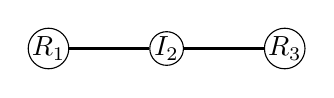
\begin{tikzpicture}[scale=1.5]
    % Draw a 7,11 network
    % First we draw the vertices
    \foreach \pos/\name in {{(1,0)/R_1}, {(2,0)/I_2}, {(3,0)/R_3}}
        \node[vertex] (\name) at \pos {$\name$};
    % Connect vertices with edges 
    \foreach \source/ \dest in {R_1/I_2, I_2/R_3}
        \path[edge] (\source) -- (\dest) ;
        
\end{tikzpicture}
%\end{minipage}
%}
\end{center}

\caption{The state and the network in which the APEX equilibrium does not exist when $k=2$.}
\label{fig:strong_connectedness}
\end{figure}

\begin{example}\label{ex_strong_connectedness}
Suppose that $k=2$ and $\theta=(R,I,R)$. The state and the network is represented in Figure~\ref{fig:strong_connectedness}. Rebel 1 never learns the type of player 3 since Inert 2 cannot reveal it. Therefore no APEX equilibrium exists in this scenario.
\end{example}

The following assumption on the prior---\textit{full support on strong connectedness}---excludes the possibility of nonexistence of APEX equilibrium. To this end, I begin with the definition of \textit{strong connectedness}.

\begin{definition}[Strong connectedness]
Given $G$, a state $\theta$ has strong connectedness if, for every two Rebels, there is a path consisting of Rebels to connect them.

\end{definition}  

In the language of graph theory, the following definition is equivalent: given $G$, $\theta$ has strong connectedness if the induced graph by $[R](\theta)$ is connected.

\begin{definition}[Full support on strong connectedness]
Given $G$, $\pi$ has full support on strong connectedness if 
\[\pi(\theta)>0\Leftrightarrow \text{ $\theta$ has strong connectedness }\] 
\end{definition}  

As a remark, the definition of the full support on strong connectedness is stronger than common knowledge about that every state has strong connectedness. This marginal requirement is subtle and is more convenient in constructing equilibrium.\footnote{The main result only requires a weaker version: $\pi(\theta)>0\Rightarrow \text{ $\theta$ has strong connectedness }$. However, working on this weaker version is at the expense of much tedious proof. Throughout this paper, I will stick to the original definition.} 

I am ready to state the main characterization of this paper:
\begin{theorem}[APEX equilibrium for the case of $1<k<n$]
\label{thm_main_result}
For any $n$-person repeated $k$-Threshold game with parameter $1<k<n$ played in networks, if networks are acyclic and if $\pi$ has full support on strong connectedness, then there is a $\delta^{*}$ such that an APEX equilibrium exists whenever $\delta>\delta^{*}$.\footnote{A network is acyclic if the path from $i$ to $j$ for all $i\neq j$ is unique.}

\end{theorem}

Constructing an APEX equilibrium in this case is convoluted. I illustrate the proof idea throughout this paper while leaving the formal proof in Appendix. Moreover, since the case of $k=2$ is trivial given that $\theta$ has strong connectedness, I focus on $2<k<n$ cases.\footnote{Suppose $[R](\theta)\geq k=2$, by the full support on strong connectedness, each Rebel have a Rebel neighbor. The following strategy is an APEX strategy. A Rebel plays \textbf{revolt} forever from period one if he has a Rebel neighbor; otherwise, he plays \textbf{stay} forever from period one. It can be extended to an APEX equilibrium by letting the out-of-path belief be: assigning probability one on the event that all non-neighbor players are Inerts.} To begin, I consider a specific APEX strategy to be the framework in constructing APEX equilibirum; incentive compatibility is not incorporated at this moment. I first study several strategies that lead at least one Rebel to learn the relevant information. 

Let us construct a set $W$ that consists of sequences of actions, in which all sequences have equal length, so that there is a one-to-one mapping between $\Theta$ and $W$. This $W$ exists because the network and the states are finite. For instance, the length of each sequence in $W$ is $n$. Given $\theta$, the $i$-th component in the corresponding $w_{\theta}$ is \textbf{revolt} if $i$ is a Rebel and is \textbf{stay} otherwise. Take another example, which is used in the constructed APEX equilibrium for Thereon~\ref{thm_main_result}, the length of each sequence in $W$ is the multiplication of a series of prime numbers. In this series, each prime number is distinct and assigned to distinct player. Denote $x_i$ as the prime number assigned to $i$. The length of a sequence is therefore $\bigotimes_{i\in N}x_i=x_1\otimes...\otimes x_n$, where $\otimes$ is the usual multiplication operator. A $\theta$ has $[R](\theta)$ Rebels, and the corresponding $w_{\theta}$ is crafted to be:  
\[(\overbrace{\textbf{stay},...,\textbf{stay},\underbrace{\textbf{revolt},\textbf{stay},...,\textbf{stay}}_{\bigotimes_{i\in [R](\theta)}x_i}}^{\bigotimes_{i\in N} x_i}).\]
There is a one-to-one mapping between $\Theta$ and ${W}$ since a multiplication of prime numbers can be uniquely factorized. The above observation is organized as follows.

\begin{proposition}
There is a set $W\subseteq \{\textbf{revolt},\textbf{stay}\}^L$, where $L\in \mathbb{N}$, so that there is a bijective mapping $f: \Theta \rightarrow W$.
\end{proposition}

Fix $W$ and then partition the time by $\{\{0\},\{1,...,s_1\},\{s_1+1,...,s_2\},...,\{s_{t-1}+1,...,s_t\},...\}$, where $t=1,2,...$ and $s_{0}=0$, so that the length of $\{s_{t-1}+1,...,s_t\}$ is equal to the length of $w\in W$ for each $t$. Call $\{s_{t-1}+1,...,s_t\}$ the $t$-block. Let $w_I\in W$ represents the state in which $I$ is the set of Rebels. Note that this $w_I$ is unique given $I$ since the state space for each player is binary. 

Given $\theta$, denote the set $I_i$ as $i$'s Rebel neighbors. If $i$ is a Rebel, let $I^1_i= I_i$, and let $I^t_i= \bigcup_{j\in G_i} I^{t-1}_j$ for $t\geq 2$. If $j$ is an Inert, let $I^t_j=\emptyset$ for $t\geq 1$. In short, $I^t_i$ is the set of Rebels who can be reached from Rebel $i$ by a path consisting of all Rebels; the length of this path is at most $t$.

The phrase, ``$i$ learn $\theta$'', indicates there is a period $s\geq 1$ so that $i$ assigns probability one to the event $\{\theta\}$ by observing histories of actions. The following proposition is immediately obtained. 
\begin{proposition}
\label{lemma:small_learn}
If $\theta$ has strong connectedness, then there is a strategy so that there exists a Rebel who can learn $\theta$.
\end{proposition}
\begin{proof} The strategy is as follows.
\[\textbf{Strategy~\ref{lemma:small_learn}:}\text{ At each $t$-block, each Rebel $i$ plays $w_{I^t_i}$}\]
By Bayesian rule, after $t$-block, Rebel $i$ assigns probability one to the event, \[\{\theta: \text{$\theta_j=R$ and $j\in I^{t+1}_i$}\}.\] To conclude the proof, the remaining is to show there exists a $t$ so that $I^{t+1}_i=[R](\theta)$. By definition, $I^t_i$ is the set of Rebels who can be reached by at most $t$ consecutive edges from Rebel $i$, in each of which the endpoints are Rebels. Since $\theta$ has strong connectedness, there exists a $t_i$ so that $I^{t_i}_i=[R](\theta)$. What follows is $i$ learn $\theta$ at $t_i$.
\end{proof}

\begin{remark}
The strong connectedness assumption in Proposition~\ref{lemma:small_learn} is indispensable as Example~\ref{ex_strong_connectedness} demonstrates. Proposition~\ref{lemma:small_learn} is essentially an if-and-only-if result.
\end{remark}

The above Strategy~\ref{lemma:small_learn} would be troublesome if incentive compatibility is under consideration, This is because tracing the expected payoff of every player in the network is a giant task. To reduce the complexity, I identify a smaller set of Rebels, \textit{active Rebels}, who are crucial in the information sharing process and thus needed to be traced. First define $G^t_i$ for each $t$: if $i$ is a Rebel, let $G^1_i= G_i$, and let $G^t_i= \bigcup_{j\in G_i} G^{t-1}_j$ for $t\geq 2$; if $j$ is an Inert, let $G^t_j=\emptyset$ for $t\geq 1$. In short, $G^t_i$ is the set of players who can be reached from Rebel $i$ by a path consisting of all Rebels; the length of this path is at most $t$. Then define the active Rebels at $t$-block as follows.
\begin{definition}[Active Rebel at $t$-block]
Set $R^0=[R](\theta)$. The set of active Rebels at $t$-block is 
\[\text{$R^t\equiv \{i\in R^{t-1}: \nexists j\in G_i \text{ such that }I^t_i\subseteq G^t_j\}$}.\]

\end{definition}
In short, an active Rebel in the $t$-block is an Rebel whose information about $\theta$, $I^t_i$, is not contained in \textit{any} Rebel's same information. For instance, in the configuration in Figure~\ref{fig:T-round-4}, $R^0=\{1,2,3,4\}$, $R^1=\{2,3\}$, and $R^2=R^3=...=\emptyset$. Furthermore, the active Rebels have to be also the active ones in the previous block; they are fewer and fewer as $t$ goes by. 

\begin{figure}

\begin{center}
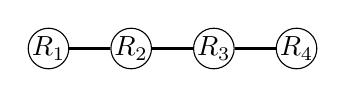
\begin{tikzpicture}[scale=0.7]
    % Draw a 7,11 network
    % First we draw the vertices
    \foreach \pos/\name in {{(1,2)/R_1}, {(2.5,2)/R_2}, {(4,2)/R_3}, {(5.5,2)/R_4}}
        \node[vertex] (\name) at \pos {$\name$};
    
%    \foreach \pos/\name in {{(2,3)/I_3}, {(5,3)/I_7}}
%    \node[unknown vertex] (\name) at \pos {$\name$};
    
%    \foreach \pos/\name in {{(3,2)/S_4}, {(4,2)/S_5}}
%    \node[selected vertex] (\name) at \pos {$\name$};
    
    % Connect vertices with edges 
    \foreach \source/ \dest in {R_1/R_2, R_2/R_3, R_3/R_4}
        \path[edge] (\source) -- (\dest) ;
        
\end{tikzpicture}
\end{center}
\caption{A configuration of the state and the network in which players 1, 2, 3, 4 are Rebels.}
\label{fig:T-round-4}
\end{figure}

\begin{lemma}
\label{lemma_inclusion}
If the $\theta$ has strong connectedness, then 
$R^t\subseteq R^{t-1}$ for all $t\geq 1$.
\end{lemma}

It is sufficient reveal the relevant information by letting only active Rebels share information about $\theta$ given that the network is acyclic and $\theta$ has strong connectedness. Theorem~\ref{lemma_empty} articulates this.
\begin{theorem}
\label{lemma_empty}
If the network is acyclic and if the $\theta$ has strong connectedness, then there is a strategy so that there exists a $R^t$ Rebel who can learn $\theta$ at $t+1$-block.
\end{theorem}
The following strategy is for Theorem~\ref{lemma_empty}. 
\[\textbf{Strategy~\ref{lemma_empty}:}\text{ At each $t$-block, each active Rebel $i$ at $t$-block plays $w_{I^t_i}$.}\] Comparing to Strategy~\ref{lemma:small_learn}, only fewer Rebels play actions to share information. Theorem~\ref{lemma_empty} is equivalent to the following statement: if the network is acyclic and if the $\theta$ has strong connectedness, then there exists $t\geq 0$ and $i\in R^t$ so that $I^{t+1}_i=[R](\theta)$.
\begin{remark}
Theorem~\ref{lemma_empty} is not true if the network is cyclic. Take the configuration in Figure\ref{fig:circle_with_bridge} as an example. There, $R^0=\{1,2,3,4,5,6\}$, $R^1=\{2,3\}$, and $R^2=R^3=...=\emptyset$. $I^2_i\neq [R](\theta)$ for all $i\in R^1$, $I^3_4=I^3_5=[R](\theta)$, but neither Rebel 4 or 5 is in $R^2$.
\end{remark}

\begin{figure}

\begin{center}
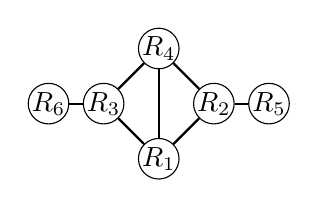
\begin{tikzpicture}[scale=0.7]
    % Draw a 7,11 network
    % First we draw the vertices
    \foreach \pos/\name in {{(2,1)/R_1}, {(3,2)/R_2}, {(1,2)/R_3}, {(2,3)/R_4}, {(4,2)/R_5}, {(0,2)/R_6}}
        \node[vertex] (\name) at \pos {$\name$};
    
%    \foreach \pos/\name in {{(2,3)/I_3}, {(5,3)/I_7}}
%    \node[unknown vertex] (\name) at \pos {$\name$};
    
%    \foreach \pos/\name in {{(3,2)/S_4}, {(4,2)/S_5}}
%    \node[selected vertex] (\name) at \pos {$\name$};
    
    % Connect vertices with edges 
    \foreach \source/ \dest in {R_1/R_4, R_1/R_2, R_1/R_3, R_2/R_4,R_3/R_4, R_2/R_5, R_3/R_6}
        \path[edge] (\source) -- (\dest) ;
        
\end{tikzpicture}
\end{center}
\caption{A configuration of the state and the network in which players 1, 2, 3, 4, 5, 6 are Rebels.}
\label{fig:circle_with_bridge}
\end{figure}

Neither Proposition~\ref{lemma:small_learn} nor Theorem~\ref{lemma_empty} affirm that all Rebels can learn the relevant information. Next, I create an APEX strategy by modifying Strategy~\ref{lemma_empty}. Fix $W$ again, but then partition the time slightly differently from the above mentioned. Partition the time by two alternating phases: \textit{coordination phase} and \textit{reporting phase}, and the time is starting from coordination phase. The $t$-th completion of two consecutive phases is called $t$-block. Figure~\ref{fig:ordered_original_game_intro} draws this partition. The length of reporting phase is equal to the length of $w\in W$, and the length of coordination phase is $2n$. The usage of reporting phase is information sharing, and the usage of coordination phase is to coordinate when the ex-post efficient outcome will be played.\footnote{More precisely, partition the time by $\{\{0\},\{1,...,s_{l_1},s_{l_1}+1,...s_1\},\{s_1+1,...,s_{l_2},s_{l_2}+1,...,s_2\},...,\{s_{t-1}+1,...,s_{l_{t}},s_{l_t}+1,...,s_t\},...\}$, where $t=1,2,...$ and $s_{0}=0$, so that the length of $\{s_{l_t}+1,...,s_t\}$ is equal to the length of $w\in W$ for each $t$, while the length of $\{s_{t-1}+1,...,s_{l_t}\}$ is $2n$. Call $\{s_{t-1}+1,...,s_t\}$ the $t$-block. call $\{s_{l_t}+1,...,s_t\}$ the \textit{reporting phase} at $t$-block and call $\{s_{t-1}+1,...,s_{l_t}\}$ the \textit{coordination phase} at $t$-block.}
\begin{figure}
\[0<\underbrace{(\text{coordination phase})<(\text{reporting phase})}_{\text{$1$-block}}<\underbrace{(\text{coordination phase})<(\text{reporting phase})}_{\text{$2$-block}}<...\]
\caption{The partition of the time in the repeated $k$-threshold game. $<$ is the linear order relation over the time.}
\label{fig:ordered_original_game_intro}
\end{figure}

\begin{proposition}
\label{lemma:small_apex}
If the network is acyclic and if the $\theta$ has strong connectedness, then there is an APEX strategy.
\end{proposition}
The following is an APEX strategy for this proposition. Suppose $T^{\theta}$ has been arrived, Rebels play the ex-post efficient outcome. Suppose $T^{\theta}$ has not yet arrived. In the reporting phase, a Rebel follows Strategy~\ref{lemma_empty}. In the coordination phase, as follows, the strategy is a contagion process. 
\begin{enumerate}
\item if a Rebel has been certain $\#[R](\theta)<k$, he plays sequence of actions $(\textbf{stay},\textbf{stay})$ continuously starting right after he was certain that, and play \textbf{stay} forever after this phase; $T^{\theta}$ is the period right after this phase.
\item if a Rebel has observed the sequence of actions $(\textbf{stay},\textbf{stay})$, he plays $(\textbf{stay},\textbf{stay})$ continuously starting right after he observed that, and plays \textbf{stay} forever after this phase; $T^{\theta}$ is the period right after this phase.
\item if a Rebel has learnt $\#[R](\theta)\geq k$, he plays sequence of actions $(\textbf{revolt},\textbf{revolt})$ continuously starting right after he learned that, and play \textbf{revolt} forever after this phase; $T^{\theta}$ is the period right after this phase.
\item if a Rebel has observed the sequence of actions $(\textbf{revolt},\textbf{revolt})$, he plays $(\textbf{revolt},\textbf{revolt})$ continuously starting right after he observed that, and plays \textbf{revolt} forever after this phase; $T^{\theta}$ is the period right after this phase.
\item if a Rebel is uncertain $\#[R](\theta)\geq k$, he plays sequence of actions $(\textbf{revolt},\textbf{stay})$ continuously.
\end{enumerate} 
The idea is simple. Rebels share information in reporting phase. If a Rebel has learnt the relevant information, he disseminates it to all Rebels contagiously in coordination phase; otherwise, he continues to reporting phase. 

If incentive compatibility is under consideration, this logic, however, brings a free-rider problem. Suppose that there are two Rebels who share information to each other in a reporting phase, and each of them is certain that he will learn the relevant information if the other one shares \textit{truthful} information to him. Due to sharing information incurs positive or negative payoff, they will not truthfully share their information. This is because each of them will choose his most profitable way of sharing information without impeding learning the relevant information provided that the other one share the truthful information. The free-rider problem turns out to be the main challenge in the construction of an APEX equilibrium. The proof solves it by arguing that if the network is acyclic, the free-rider problem only occurs between two Rebel neigbors who \textit{commonly know it}, while this argument does not hold for cyclic network.\footnote{Section~\ref{sec:cyclic} provides an example that the free-rider problem is not commonly known between the Rebels who involve.} 
With the help from this argument, the constructed equilibrium solves the free-rider problem by arbitrarily assigning one of them to be the {free rider}, who can choose his most profitable way in sharing information, while letting the other one share truthful information. 

%To make the discussion of incentive compatibility more transparent, I introduce \textit{$T$-round writing game} as an auxiliary scenario. In the $T$-round writing game, $T$ is fixed, players are endowed a writing technology so that they can write to share information about $\theta$ for $T$ rounds. They then play a one-shot $k$-threshold game at round $T+1$. This game is a reduced form of the original game by fixing $T$, so that I can pay attention only to the incentive compatibility in information sharing process and ignore how players determine the terminal period. This writing technology represent a way of communication by \textit{writing sentences that are composed by letters according to a fixed grammar}. Though this auxiliary game will be soon introduced in the next section, I draw Table~\ref{table:analogue} to shed light on the parallel between it and the original game.
%
%\begin{table}[!htbp]
%\caption{The analogue between $T$-round writing game and the repeated $k$-threshold game}
%\label{table:analogue}
%\begin{center}
%\begin{tabular}{cc }
%$T$-round writing game & Repeated $k$-threshold game \\
%\hline
%\hline
%A round & A range of periods\\
%A sentence & A sequence of actions \\
%The length of a sentence in a round & The length of a range of periods\\
%A chosen letter in a sentence & A chosen action\\
%The cost of writing a sentence & The expected payoff occurring in a sequence of actions\\
%The fixed grammar & The equilibrium path\\
%\hline
%\end{tabular}
%\end{center}
%
%\end{table}
%
%%In short, constructing an APEX equilibrium amounts to creating a framework for players in sharing information before $T^{}$ and determining the terminal period $T^{\theta}$ by themselves. Due to imperfect monitoring, one major challenging is to manage players' higher-order belief over others' actions as well as the induced belief over states. I solve it by heavily exploiting the implicit assumption underlying the infinite repeated game: the time is ``synchronized;'' at every period, players commonly know that they are in that period. Taking advantage of it, I partition the time by a collection $\mathbb{T}=\{\Tau_1,\Tau_2,...\}$ so that each generic element is a range of periods.\footnote{To be precise, $\Tau_{\xi}\subset \{1,2,...\}$, $\Tau_{\dot{\xi}}\cap\Tau_{\ddot{\xi}}=\emptyset$ for $\dot{\xi},\ddot{\xi}=1,2,...$, and $\bigcup_{\xi\in\{1,2,...\}}\Tau_{{\xi}}=\{1,2,...\}$.} During the game, players know that they are in $\Tau_{\xi}$ for some $\xi$. On the equilibrium path, players play specific sequences of actions with the length of $\Tau_{\xi}$ for some $\xi$ they are in. There are two subsets $\Tau,\Tau^{'}\in \mathbb{T}$. $\Tau$ is meant to be the periods for sharing information and $\Tau^{'}$ is meant to be the periods for spreading the knowledge about relevant information. Elements in $\Tau$ and elements in $\Tau^{'}$ occur in turns in the time horizontal line. If not all of Rebels find the relevant information revealed in an element in $\Tau^{'}$, all Rebels will enter the next range of periods, which is an element in $\Tau$, to share information. After that, all of them will enter the next range of periods, which is an element in $\Tau^{'}$, to see whether the relevant information will be revealed. If not, they enter the next element in $\Tau$,...., and keep doing so until the terminal period $T^{\theta}$ is reached.  
%
%
%%An APEX equilibrium thus amounts to sharing information before $T^{}$ and determining $T^{\theta}$ by Rebels themselves. Some observations follows. Firstly, since a Rebel has only two actions but the relevant information involves the number of Rebels, a Rebel must play sequences of actions to represent ``bigger'' information, say the number of $7$.\footnote{Especially, playing so can represent the information about the locations of Rebels by exploiting the finite network and the common knowledge of the network.} Due to this, the answers to how many sequences or how long a sequence they would use and what $T^{\theta}$ is are not obvious before the equilibrium is constructed. Secondly, due to the imperfect monitoring, it is elaborate to describe every player's infinite higher-order belief over other players' histories of actions, as well as the belief over states for every player.
%
%
%  
%
%%In the case of $k=n$, $T^{\theta}$ can be determined independently from $\theta$ by setting $T^{\theta}=n$, but it is not obvious how to obtain $T^{\theta}$ before an equilibrium has been constructed.\footnote{Readers might refer to the proof of Theorem~\ref{thm_minor_thm}.} 
%%Moreover, the free-rider problem might exist in the current case (as demonstrated in Introduction), but this problem never occurs in the proposed APEX equilibrium for Theorem~\ref{thm_minor_thm}. As for the punishment scheme, playing \textbf{stay} forever is not effective anymore since a deviation might only be seen by parts of players (network monitoring), and thus group punishment is hard to be executed.
%
%%Before we delve further into the logic of the proof of Theorem 2, I would like to introduce a game in Section~\ref{sec:writing}: \textit{$T$-round writing game}. This is a simpler auxiliary scenario that mimics relevant features in the original game. In the $T$-round writing game, I allow players to write to each other. They will be endowed a writing technology so that they can write without cost (cheap talk) or with a cost function before they take actions. 
%% 
%%%The equilibrium construction of $T$-round writing game will be studied by means of examples and intentionally serve to demonstrate how to solve the free-rider problem. I then argue the equilibrium construction in the original game to be an analogue to the one in the $T$-round writing game. 
%%
%%Roughly speaking, in the $T$-round writing game, players can write to share information about $\theta$ for $T$ rounds. They then play a one-shot $k$-threshold game at round $T+1$. Note that in an APEX equilibrium path in the original game, players would stop updating their belief after some finite time and keep playing the same action in the $k$-threshold game. The game form of the $T$-round writing game mimics the structure of the APEX equilibrium path in the original game. In Section~\ref{sec:indem_writing}, I then further modify the $T$-round writing game to allow $T$ to be endogenously determined in the equilibrium, which is seamlessly analogous to the original game.\footnote{TBA.}  
%
%  
%
%\subsection{$T$-round writing game}
%\label{sec:writing}
%The network, the set of states, and the set of players follow exactly the same definitions defined in Section~\ref{sec:model}. In the $T$-round writing game, each player endows a \textit{writing technology}. A writing technology for player $i$ is a pair of $(W,M_i)$, in which $W=\{{\textbf{r}},\textbf{s}\}^L$, $L\in \mathbb{N}$, and $M\equiv \bigtimes_{i\in N}\bigtimes^T_{t=1}M^{t}_i$ recursively defined by
%\[M^1_i=\{f|f:\Theta_{G_i}\rightarrow W\}\cup \{\emptyset\}\]
%\[ \text{ for } 2\leq t \leq T\text{ , }M^{t}_i=\{f|f:\bigtimes_{j\in G_i}M^{t-1}_j\rightarrow W\}\cup \{\emptyset\}. \]
%$W$ is interpreted as the set of sentence composed by letters \textbf{r} or \textbf{s} with length $L$, while $M_i$ is understood as $i$'s grammar. $\emptyset$ represents remaining silent. The phrase of ``$i$ writes a sentence to all his neighbors at round $t$'' is equivalent to ``$i$ selects an $f\in M^t_i$ to get an element $w\in W$ according to $f$, which can be observed by all $i$'s neighbors''. 
%%A sentence being a mixture of two sentences $w,w^{'}\in W$ is denoted as $w\oplus w^{'}$ with the property that $(w\oplus w^{'})_l=\textbf{r}$ if and only if $w_l=\textbf{r}$ or $w^{'}_l=\textbf{r}$ for all $l\in \{1,...,L\}$. 
%
%The time line for the deterministic $T$-round writing game is as follows.
%\begin{enumerate}
%\item Nature chooses $\theta$ according to the prior $\pi$.
%\item $\theta$ is then fixed throughout rounds.
%\item At $t=1,...,T$ round, players write to their neighbors. 
%\item At $T+1$ round, players play a one-shot $k$-Threshold game.
%\item The game ends.
%\end{enumerate}
%%\begin{table}[!htbp]
%%\begin{center}
%%\begin{tabular}{ll }
%%1.  & Nature chooses $\theta$ according to $\pi$. \\
%%2. & $\theta$ is then fixed throughout rounds.\\
%%3. & At $t=1,...,T$ round, players write to their neighbors. \\
%%4. & At $T+1$ round, players play a one-shot $k$-Threshold game.\\
%%5. & The game ends.
%%\end{tabular}
%%\end{center}
%%\end{table}
%A Rebel's payoff is the summation of his stage payoff across stages, while an Inert's payoff is set to be $1$. The equilibrium concept is weak sequential equilibrium. An APEX strategy is a strategy that induces the ex-post outcome in the one-shot $k$-threshold game at $T+1$ round. The definition of APEX equilibrium is adapted accordingly. In the examples below, let us focus on the configuration represented in Figure~\ref{fig:T-round-6} and Figure~\ref{fig:T-round-5} with $n=L=8$. I.e.~there are 8 players and the length of a sentence is also 8. Note that the differences between configurations in Figure~\ref{fig:T-round-6} and Figure~\ref{fig:T-round-5} are: (1) $\#[R](\theta)=6$ in Figure~\ref{fig:T-round-6} but $\#[R](\theta)=5$ in Figure~\ref{fig:T-round-5}; (2) player 8 is a Rebel in Figure~\ref{fig:T-round-6} but he is an Inert in Figure~\ref{fig:T-round-6}.
%
%\begin{figure}
%
%\begin{center}
%\begin{tikzpicture}[scale=0.7]
%    % Draw a 7,11 network
%    % First we draw the vertices
%    \foreach \pos/\name in {{(1,2)/R_1}, {(2,1)/R_2}, {(5,1)/R_6}, {(6,2)/R_8}, {(3,2)/R_4}, {(4,2)/R_5}}
%        \node[vertex] (\name) at \pos {$\name$};
%    
%    \foreach \pos/\name in {{(2,3)/I_3}, {(5,3)/I_7}}
%    \node[unknown vertex] (\name) at \pos {$\name$};
%    
%%    \foreach \pos/\name in {{(3,2)/S_4}, {(4,2)/S_5}}
%%    \node[selected vertex] (\name) at \pos {$\name$};
%    
%    % Connect vertices with edges 
%    \foreach \source/ \dest in {R_1/R_4, R_2/R_4,I_3/R_4,R_4/R_5, R_5/R_6, R_5/I_7, R_5/R_8}
%        \path[edge] (\source) -- (\dest) ;
%        
%\end{tikzpicture}
%\end{center}
%\caption{A configuration of the state and the network in which players 1, 2, 4, 5, 6, 8 are Rebels while players 3, 7 are Inerts.}
%\label{fig:T-round-6}
%\end{figure}
%
%\begin{figure}
%
%\begin{center}
%\begin{tikzpicture}[scale=0.7]
%    % Draw a 7,11 network
%    % First we draw the vertices
%    \foreach \pos/\name in {{(1,2)/R_1}, {(2,1)/R_2}, {(5,1)/R_6}, {(3,2)/R_4}, {(4,2)/R_5}}
%        \node[vertex] (\name) at \pos {$\name$};
%    
%    \foreach \pos/\name in {{(2,3)/I_3}, {(5,3)/I_7}, {(6,2)/I_8}}
%    \node[unknown vertex] (\name) at \pos {$\name$};
%    
%%    \foreach \pos/\name in {{(3,2)/S_4}, {(4,2)/S_5}}
%%    \node[selected vertex] (\name) at \pos {$\name$};
%    
%    % Connect vertices with edges 
%    \foreach \source/ \dest in {R_1/R_4, R_2/R_4,I_3/R_4,R_4/R_5, R_5/R_6, R_5/I_7, R_5/I_8}
%        \path[edge] (\source) -- (\dest) ;
%        
%\end{tikzpicture}
%\end{center}
%\caption{A configuration of the state and the network in which players 1, 2, 4, 5, 6 are Rebels while players 3, 7, 8 are Inerts.}
%\label{fig:T-round-5}
%\end{figure}
%
%%
%%\subsubsection{$T$-round writing game with cheap talk}
%%\label{sec:cheap_talk}
%%\begin{example}[Deterministic $T$-round writing without cost---cheap talk]
%%\label{ex:cheap_talk}
%%Let $k=6$, $T=2$, and suppose writing is costless. This is, there are two rounds for writing, while writing is the same as cheap talk.
%%%Let the grammar for Rebel 4 (or 5) be: \textbf{r} is written in the $i$-th component if player $i$ is a Rebel; \textbf{s} is written in the $j$-th component if $j$'s type is an Inert or unknown to Rebel 4 (or 5).
%%
%%Consider the following strategy $\phi$. 
%%
%%At $t=1$, the peripheral Rebels remain silent. Rebel 4 (or 5)'s grammar for writing a sentence is: if player $i$ is a Rebel and known to him, he writes \textbf{r} in the $i$-th component in the sentence; otherwise, he writes \textbf{s} in that component. According to this grammar, the central player Rebel 4 writes the sentence $(\textbf{r},\textbf{r},\textbf{s},\textbf{r},\textbf{r},\textbf{s},\textbf{s},\textbf{s})$ on both configurations in Figure~\ref{fig:T-round-6} and in Figure~\ref{fig:T-round-5}. The central player Rebel 5 writes $(\textbf{s},\textbf{s},\textbf{s},\textbf{r},\textbf{r},\textbf{r},\textbf{s},\textbf{r})$ in the configuration in Figure~\ref{fig:T-round-6} and writes $(\textbf{s},\textbf{s},\textbf{s},\textbf{r},\textbf{r},\textbf{r},\textbf{s},\textbf{s})$ in the configuration in Figure~\ref{fig:T-round-5}.\footnote{The notion of ``peripheral'' and ``central'' will be formalized in Section~\ref{sec:info}} Rebels 4 and 5's sentences thus reveals who are Rebels and who are not. Notice that the common knowledge of the network contributes to the ability of revealing players' types. 
%%
%%At $t=2$, the peripheral Rebels still remain silent. Rebel 4 writes $(\textbf{r},\textbf{r},\textbf{s},\textbf{r},\textbf{r},\textbf{r},\textbf{s},\textbf{r})$ in the configuration in Figure~\ref{fig:T-round-6} and writes $(\textbf{r},\textbf{r},\textbf{s},\textbf{r},\textbf{r},\textbf{r},\textbf{s},\textbf{s})$ in the configuration in Figure~\ref{fig:T-round-5}. Rebel 5 writes exactly the same sentence as Rebel 4. This is to say Rebel 4 and 5 share information at $t=1$ and then coordinate to announce a mixture sentence at $t=T$. 
%%
%%At $T+1$, by counting \textbf{r} in Rebel 4 or 5's mixture sentence, all Rebels know whether the number of Rebels outnumbers $k$. This leads all Rebels to play the ex-post efficient outcome in the one-shot $k$-threshold game. 
%%
%%%Suppose the configuration is that in Figure~\ref{fig:T-round-5}. At $t=1$, similarly, $\phi$ specifies that Rebels 1,2,6,8 keep silent; Rebel 4 writes $(\textbf{r},\textbf{r},\textbf{s},\textbf{r},\textbf{r},\textbf{s},\textbf{s},\textbf{s})$; Rebel 5 writes $(\textbf{s},\textbf{s},\textbf{s},\textbf{r},\textbf{r},\textbf{r},\textbf{s},\textbf{s})$. At $t=2$, however, $\phi$ specifies that the peripheral Rebels 1,2,6,8 keep silent; Rebel 4 keeps silent; Rebel 5 keeps silent as well. On the path, keeping silent by Rebel 4 (or 5) reflects that Rebel 4 (or 5) knows that the total number of Rebels is less than $k=6$. At $t=3$, all Rebels know this relevant information and play the ex-post efficient outcome \textbf{stay}.
%%
%%
%%\end{example}
%%
%%\begin{remark}
%%An assessment $(\phi,\omicron)$, where $\omicron$ is a belief system, is made to be an APEX equilibrium for Example~\ref{ex:cheap_talk} above as follows. The out-of-path strategy of $\phi$ specifies that if there is a detectable deviation, then the Rebels who detect this deviation will remain silent until $t=T$ and then play \textbf{stay} at $T+1$.\footnote{A deviation could be, for instance, a wrong sentence that is not grammatical, is deviating from the in-path $\phi$,..., etc} 
%%The out-of-path belief of $\omicron$ is to believe that all players who are not neighbors are Inerts. The in-path belief of $\omicron$ is the belief induced by $\phi$. Since any deviation by Rebel 4 or 5 would strictly decrease the possibility of achieving an ex-post efficient outcome, and writing is costless, the assessment $(\phi,\omicron)$ constitutes an APEX equilibrium.
%%\end{remark}
%%\begin{example}[Deterministic $T$-round writing with a fixed cost]
%%\label{ex:fixed_cost_talk}
%%Let $k=6$ and $T=2$. Suppose that writing incurs a fixed cost $\epsilon>0$ while keeping silent does not. Let us consider the assessment $(\phi,\omicron)$ in the above example. Since any deviation by Rebel 4 or 5 would strictly decrease the possibility to achieve the ex-post efficient outcome while the ex-post efficient outcome will give the maximum expected payoff for every Rebel at $t=3=T+1$ if the relevant information can be revealed then, if $\epsilon$ is sufficiently small, $(\phi,\omicron)$ also constitutes an APEX equilibrium.
%%
%%\end{example}
%
%%If writing is costly instead, the next example shows that $(\phi,\omicron)$ is not an APEX equilibrium. This is due to the free-rider problem.
%
%\begin{example}[$T$-round writing and the free-rider problem]
%\label{ex:cost_function_talk_fr}
%Let $k=6$ and $T=2$. Suppose that remaining silent incurs no cost, but writing incurs an extremely small cost $\epsilon>0$ so that $\epsilon$ is strictly decreasing with the number of \textbf{r} in a sentence. This is to say writing $(\textbf{r},\textbf{r},\textbf{r},\textbf{r},\textbf{r},\textbf{r},\textbf{r},\textbf{r})$ incurs the least cost while writing $(\textbf{s},\textbf{s},\textbf{s},\textbf{s},\textbf{s},\textbf{s},\textbf{s},\textbf{s})$ incurs the largest. 
%
%Consider the following strategy $\phi$. 
%
%At $t=1$, the peripheral Rebels remain silent. Rebel 4 (or 5)'s grammar for writing a sentence is that if player $i$ is a Rebel and known to him, he writes \textbf{r} in the $i$-th component in the sentence; otherwise, he writes \textbf{s} in that component. According to this grammar, the central player Rebel 4 writes the sentence $(\textbf{r},\textbf{r},\textbf{s},\textbf{r},\textbf{r},\textbf{s},\textbf{s},\textbf{s})$ on both configurations in Figure~\ref{fig:T-round-6} and in Figure~\ref{fig:T-round-5}. The central player Rebel 5 writes $(\textbf{s},\textbf{s},\textbf{s},\textbf{r},\textbf{r},\textbf{r},\textbf{s},\textbf{r})$ in the configuration in Figure~\ref{fig:T-round-6} and writes $(\textbf{s},\textbf{s},\textbf{s},\textbf{r},\textbf{r},\textbf{r},\textbf{s},\textbf{s})$ in the configuration in Figure~\ref{fig:T-round-5}. Rebels 4 and 5's sentences thus reveals who are Rebels and who are not. Notice that the common knowledge of the network contributes to the ability of revealing players' types. 
%
%At $t=2$, the peripheral Rebels still remain silent. Rebel 4 writes $(\textbf{r},\textbf{r},\textbf{s},\textbf{r},\textbf{r},\textbf{r},\textbf{s},\textbf{r})$ in the configuration in Figure~\ref{fig:T-round-6} and writes $(\textbf{r},\textbf{r},\textbf{s},\textbf{r},\textbf{r},\textbf{r},\textbf{s},\textbf{s})$ in the configuration in Figure~\ref{fig:T-round-5}. Rebel 5 writes exactly the same sentence as Rebel 4. This is to say Rebel 4 and 5 share information at $t=1$ and then coordinate to announce a mixture sentence at $t=T$. 
%
%At $T+1$, by counting \textbf{r} in Rebel 4 or 5's mixture sentence, all Rebels know whether the number of Rebels outnumbers $k$. This leads all Rebels to play the ex-post efficient outcome in the one-shot $k$-threshold game. 
%
%The above $\phi$ is not an APEX equilibrium. According to the above-mentioned, Rebel 4 will know the relevant information at $t=2$ even if he deviates to writing that all his neighbors are Rebels, which incurs less cost than his truthful writing.\footnote{This sentence is $(\textbf{r},\textbf{r},\textbf{r},\textbf{r},\textbf{r},\textbf{s},\textbf{s},\textbf{s})$, which incurs less cost than the truthfully reporting sentence $(\textbf{r},\textbf{r},\textbf{s},\textbf{r},\textbf{r},\textbf{s},\textbf{s},\textbf{s})$.}\footnote{If he remains silent, then this behavior will be considered as a deviation, and therefore he will never get the maximum payoff of $1$. Hence, he will avoid doing so.}
%Rebel 5 is in the same situation as Rebel 4 and therefore also writes the sentence that indicates that all his neighbors are Rebels. However, these sentences are uninformative. It turns out that both of them will deviate, and neither of them can know the relevant information at $t=2$.
%%\footnote{Actually, one can claim there is no APEX equilibrium in this case by contraposition. If there is one, say $(\phi^{'},\omicron^{'})$, then on the path of $\phi^{'}$, some Rebels should write and play differently in different configurations. Suppose Rebel 5 will play differently to truthfully reveal his information at $t=1$. Rebel 4 has two kinds of strategies then. He might write the least-cost sentence or he could write something depending on his information. For the former case, since Rebel 4 will be the only one who know the relevant information, he should write to Rebel 5 to let Rebel 5 pass this information to the remaining Rebels. However, it requires two rounds to pass it, but there is only one round left. For the latter case, if Rebel 4 truthfully reveal his information, the Rebel 5 will deviate to writing least-cost sentence; if Rebel 4's information is not truthfully reveal, there is a prior so that the ex-post outcome will not be played.}
%
%
%\end{example}
%
%Fortunately, the following example shows that the free-rider problem can be solved. 
%
%\begin{example}[$T$-round writing and solving the free-rider problem]
%\label{ex:cost_function_talk_solve_fr}
%The solution to solve the free-rider problem in the previous example is to extend $T$. It would open the possibility of the existence of a free rider at some round, while letting this free rider reveals relevant information at the next round. To this end, let $k=6$ and $T=3$. Consider the following strategy $\rho$ and focus on the interaction between Rebels 4 and 5.
%%First note that if the previous strategy $\phi$ is extended to the current case so that Rebel 4 and 5 still simultaneously truthfully write their information at either $t=1$ or $t=2$, $\phi$ is not an equilibrium path by the same free-rider argument as the above. 
%
%At $t=1$, the lowest-index Rebel between Rebels 4 and 5 is the free rider, while the other one truthfully writes down his information. This is to say Rebel 4 will be the free rider and he writes the least-cost sentence. Rebel 5 writes $(\textbf{s},\textbf{s},\textbf{s},\textbf{r},\textbf{r},\textbf{r},\textbf{s},\textbf{r})$ in the configuration of Figure~\ref{fig:T-round-6}and writes $(\textbf{s},\textbf{s},\textbf{s},\textbf{r},\textbf{r},\textbf{r},\textbf{s},\textbf{s})$ in the configuration of Figure~\ref{fig:T-round-5}. 
%
%At $t=2$, Rebel 4 has known the relevant information. Rebel 4 writes the least-cost sentence if $\#[R](\theta)\geq k$ but remains silent otherwise. The consequence is Rebel 4's behavior reveals the relevant information to his neighbors at this round. Rebel 5 remains silent instead. 
%
%At $t=T$, Rebel 5 has known the relevant information since he is Rebele 4's neighbor. He writes the least-cost sentence if $\#[R](\theta)\geq k$ but remains silent otherwise. Therefore Rebel 5's behavior at this round reveals the relevant information to his neighbors. Rebel 4 remains silent instead.
%
%At $T+1$, all Rebels know the relevant information by observing Rebels 4 and 5's behavior. They play the ex-post efficient outcome accordingly. 
%%To construct an APEX equilibrium from $\rho$, recall $(\phi,\omicron)$ and let the in-path belief of $\dot{\omicron}$ be induced by $\rho$. The out-of-path strategy follows that in $\phi$, and the out-of-path belief follows that of $\omicron$.   
%
%
%
%\end{example}
%
%\begin{remark}
%Why does Rebel 5 \textit{know} that he is not a free rider and therefore behaves not like a free rider? The following is the reason. He \textit{knows} that, by common knowledge of the network, he and Rebel 4 are in a free-rider problem. Moreover, by common knowledge of the network, he knows that Rebel 4 knows that he and Rebel 4 are in a free-rider problem, he knows that Rebels 4 knows that he knows that,...,and so forth. Consequently, Rebel 5 and 4 commonly know that they are engaged in a free-rider problem. Lemma~\ref{lemman_pivotals_CK} articulate a general result: engaging in a free-rider problem is a common knowledge between Rebels who involve for any acyclic network in the constructed APEX equilibrium. Lemma~\ref{lemman_pivotals_CK} is, however, false in cyclic networks. Example~\ref{ex:cyclic} discusses this issue.
%\end{remark}
%
%%Next, I allow $T$ is not fixed; players have to determine what $T$ is by themselves. I organize the discussion in the next section.
%
%%\subsection{Indeterministic $T$-round writing game}
%%\label{sec:indem_writing}
%%The setting here is exactly the same as in the deterministic $T$-round writing game, except for that there are infinite rounds and players have to jointly decide when they will play the one-shot $k$-threshold game. They have to {reach an agreement}---the common knowledge of which round the terminal round ${T}$ is. 
%%
%%The set of rounds is countably infinite with generic element $t$ and linearly ordered. The writing technology is the same as that in deterministic $T$-round writing game, except for there are sentences different in their length: $W=\{\textbf{r},\textbf{s}\}^L\cup \{\textbf{r},\textbf{s}\}^{L^{'}}$. 
%%
%%Conceptually, there could be two kinds of rounds. In the first kind, players write to share information about $\theta$. In the second kind, players write to form the common knowledge about ${T}$. Let us partition the set of rounds into two parts, $\Gamma$ and $\Gamma^{'}$, which represent the first kind and the second kind respectively. The round in $\Gamma$ is labelled $\gamma\in\{1,2,...\}$. The round in $\Gamma^{'}$ is labelled $\gamma^{'}_{l_\gamma}$, where $\gamma^{'}\in \{0^{'},1^{'},...\}$ and $l_{\gamma}\in\{1,2,....\}$ for $\gamma=0,1,...$. The rounds are linearly ordered by $<$. Specifically, the rounds and their labelling are ordered as shown in Figure~\ref{fig:ordered_writing}.
%%\begin{figure}
%%\begin{center}
%%\[0^{'}_1<0^{'}_2<...<0^{'}_{l_0}<1<1^{'}_{1}<1^{'}_{2}<...<1^{'}_{l_1}<2<...,\]
%%where $l_0,l_1,...$ are all finite numbers.
%%\caption{The linearly ordered rounds in the indeterministic $T$-round writing game.}
%%\label{fig:ordered_writing}
%%\end{center}
%%\end{figure}
%%
%%%An indeterministic $T$-round writing game is illustrated below. Along with it, an APEX equilibrium will be constructed. 
%%
%%\begin{example}[Indeterministic $T$-round writing with cost function]
%%\label{ex:cost_function_talk_solve_fr_Indm}
%%Let $k=6$ and $l_{\gamma}=2$ for $\gamma=0,1,...$. Let us consider the following strategy $\psi$. At a round in $\Gamma^{'}$, $\psi$ specifies that, 
%%\begin{itemize}
%%\item if a Rebel thinks ``He is certain that $\#[R](\theta)\geq k$ and the nearest forthcoming round in $\Gamma$ is the terminal round,'' he will write $(\textbf{r})$;
%%\item if a Rebel thinks ``He is uncertain about $\# [R](\theta)\geq k$,'' he will write $(\textbf{s})$;
%%\item otherwise, if a Rebel think ``$\#[R](\theta)\geq k$ is impossible and the nearest forthcoming round in $\Gamma$ is the terminal round,'' he will write $\emptyset$. 
%%\end{itemize}
%%
%%According to this strategy, $t=1$ is not terminal in the configuration in Figure~\ref{fig:T-round-6} or Figure~\ref{fig:T-round-5} since all Rebels writes $(\textbf{s})$ at $t=0^{'}_1,0^{'}_2$. 
%%
%%At $t=1$, Rebels 4 and 5 are in a free-rider problem at $t=1$. $\psi$ solves it by letting Rebel 4 be the free rider and Rebel 5 write his information truthfully. 
%%
%%At $t=1^{'}_1$, Rebel 4 knows $\#[R](\theta)\geq k$ in the configuration in Figure~\ref{fig:T-round-6} and knows $\#[R](\theta)< k$ in the configuration in Figure~\ref{fig:T-round-5}. Therefore, he writes $(\textbf{r})$ in the configuration in Figure~\ref{fig:T-round-6} and $\emptyset$ in the configuration in Figure~\ref{fig:T-round-5}. As for other Rebels, they write $(\textbf{s})$. 
%%
%%At $t=1^{'}_2$, all Rebels will learn the relevant information by observing what Rebel 4 writes at $t=1^{'}_1$. They terminate their writing at $t=2$ since they have learnt the relevant information. Therefore, $t=2$ is the terminal round, and the Rebels play a one-shot $k$-threshold game at $t=3$.
%%
%%The strategy $\psi$ can be made to be an APEX equilibrium strategy in the same way as Example~\ref{ex:cheap_talk}. 
%%
%%
%%\end{example}


%\subsection{Equilibrium path and the out-of-path belief}
%\label{sec:dis_writing}
I then delver into substantial details in constructing an APEX equilibrium. The framework is adapted from Proposition~\ref{lemma:small_apex}, and the time is again partitioned by two alternating phases as shown in Figure\ref{fig:ordered_original_game_intro}. The out-of-path belief is simple, which serves as a grim trigger. Whenever Rebel $i$ detects a deviation at period $\varsigma$, he forms the following belief: 
\begin{equation}
\label{eq_grim_trigger}
\sum_{\theta \in \{\theta:\theta_j=I,j\notin G_i\}}\beta^{\pi,\tau}_{G_i}({\theta}|h^{s}_{G_i})=1 \text{, for all $s\geq \varsigma$}.
\end{equation}
Thus, if $\# I^{\varsigma}_i<k$, he will play \textbf{stay} forever after he detects a deviation. This out-of-path belief thus serves as a grim trigger. 
%To fix the idea, I draw analogue between the writing game and the original game in Table~\ref{table:analogue}. 

%In the equilibrium construction in the original game, let us partition the periods so that each part in the partition is analogous to a round in the writing game. The length of periods in a part is analogous to the length of a sentence. Since the actions played in a certain part of periods will incur an expected payoff, it is an analogue that writing is costly at a certain round in the writing game. The disjoint unions of period-sections also constitute a coarser partition of periods, which is analogous to partitioning the rounds. The analogue of $\Gamma$ is the set of \textit{reporting phase} in the original game to emphasize that these periods are for reporting information about $\theta$. The analogue of $\Gamma^{'}$ is the set of \textit{coordination phase} in the original game to emphasize that these periods are for coordinating to play the ex-post efficient outcome. The partition of periods is linearly ordered by $<$, and let us define a coarser partition with parts \textit{$t$-blocks} indexed by $t\in\{0,1,...\}$ along with the order of partition of periods as shown in Figure~\ref{fig:ordered_original_game}. 

%In the equilibrium construction in the original game, let us partition the periods so that it is analogous to partitioning the rounds. The analogue of $\Gamma$ is the set of \textit{reporting phase} in the original game to emphasize that these periods are for reporting information about $\theta$. The analogue of $\Gamma^{'}$ is the set of \textit{coordination phase} in the original game to emphasize that these periods are for coordinating to play the ex-post efficient outcome. The partition of periods is linearly ordered by $<$, and let us define a coarser partition as \textit{$t$-blocks} indexed by $t\in\{0,1,...\}$ along with the order of partition of periods as shown in Figure~\ref{fig:ordered_original_game}.  

%\begin{figure}
%\[\underbrace{(\text{coordination phase})}_{\text{$0$-block}}<\underbrace{(\text{reporting phase})<(\text{coordination phase})}_{\text{$1$-block}}<...\]
%\caption{The linearly ordered period-sections in the repeated $k$-threshold game.}
%\label{fig:ordered_original_game}
%\end{figure}









%\subsubsection{Information hierarchy}
%\label{sec:info}
%The information hierarchy across players presents players' information \textit{before} entering the reporting phase at $t$-block. That is a tuple \[(\{G^{t}_i\}_{i\in N}, \{I^{t}_i\}_{i\in N}, R^t,\theta).\]
%$G^{t}_i$ represents \textit{$i$'s extended neighbors}: $j\in G^{t}_i$ if $j$ can be reached by at most $t$ consecutive edges from a Rebel $i$ so that the endpoints of $t-1$ edges are both Rebels. $I^{t}_i$ represents \textit{$i$'s information about $\theta$}: the set of Rebels in $G^t_i$. $R^t$ represents \textit{the active Rebels}: those Rebels whose information about $\theta$ is not included any of their neighbor. Those objects are defined by:
%
%At $0$-block,
%\[\text{if $\theta_i=I$, $G^{0}_i\equiv \emptyset$, $I^{0}_i\equiv \emptyset$.}\] 
%\[\text{if $\theta_i=R$, $G^{0}_i\equiv \{i\}$, $I^{0}_i\equiv \{i\}$.}\] 
%\[\text{$R^0\equiv [R](\theta)$.}\] 
%
%At $1$-block,
%\[\text{if $\theta_i=I$, $G^{1}_i\equiv \emptyset$, $I^{1}_i\equiv \emptyset$.}\] 
%\[\text{if $\theta_i=R$, $G^{1}_i\equiv G_i$, $I^{1}_i\equiv G_i\cap R^0$.}\] 
%\[\text{$R^1\equiv \{i\in R^0: \nexists j\in G_i \text{ such that }I^1_i\subseteq G^1_j\}$.}\] 
%
%At $t$-block for $t>1$, 
%\[\text{if $\theta_i=I$, $G^{t}_i\equiv \emptyset$, $I^{t}_i\equiv \emptyset$.}\] 
%\[\text{if $\theta_i=R$, $G^{t}_i\equiv \bigcup_{j\in G_i} G^{t-1}_j$, $I^{t}_i\equiv \bigcup_{j\in G_i} I^{t-1}_j$, }\] 
%\[\text{$I^{t}_{ij}\equiv I^{t-1}_i\cap I^{t-1}_j$ if $j\in G_i$.}\]
%\[\text{$R^t\equiv \{i\in R^{t-1}: \nexists j\in G_i \text{ such that }I^t_i\subseteq G^t_j\}$.}\]
%
%
%
%According to the definition above, the peripheral Rebels in the configuration of Figure~\ref{fig:T-round-6} are active in $0$-block (in $R^0$) but not active in $1$-block (not in $R^1$), while the central players are active in both $0$-block and $1$-block. It can be shown that $R^t\subseteq R^{t-1}$ as follows. 
%\begin{lemma}
%\label{lemma_inclusion}
%If the $\theta$ has strong connectedness, then 
%\[R^t\subseteq R^{t-1}\] for all $t\geq 1$.
%\end{lemma}
%
%Is it sufficient to let only active Rebels share information about $\theta$ while $\theta$ can be revealed eventually? The answer is affirmative proven by Theorem~\ref{lemma_empty} below, if the network is acyclic and if the $\theta$ has strong connectedness.
%\begin{theorem}
%\label{lemma_empty}
%If the network is acyclic and if the $\theta$ has strong connectedness, then 
%\[[R](\theta)\neq \emptyset \Rightarrow \text{ there exists } t\geq 0 \text{ and } i\in R^t \text{ such that }I^{t+1}_i=[R](\theta).\] 
%\end{theorem}
%
%
%The strategy on the equilibrium path will specify how Rebels act according to the information hierarchy. $R^t$ will be those Rebels who are active in terms of sharing information in the reporting phase in the $t$-block. 

%For convince, let us denote $I^{t+1}_{ij}=I^t_i\cap I^t_j$ if $j\in G_i\cap R^{t}$.  


%\subsubsection{Out-of-path belief}
%I depict the out-of-path belief. Whenever Rebel $i$ detects a deviation at period $\varsigma$, he forms the following belief: 
%\begin{equation}
%\label{eq_grim_trigger}
%\sum_{\theta \in \{\theta:\theta_j=I,j\notin G_i\}}\beta^{\pi,\tau}_{G_i}({\theta}|h^{s}_{G_i})=1 \text{, for all $s\geq \varsigma$}.
%\end{equation}
%Thus, if $\# I^1_i<k$, he will play \textbf{stay} forever after he detects a deviation. This out-of-path belief serves as a grim trigger. 


\subsection{The equilibrium path in the reporting phase}
\label{sec:eq_rp}
If there is no further mention, all the description in this section is for the APEX equilibrium path \textit{before} the terminal period $T^{\theta}$. Let us shorten ``reporting phase in $t$-block'' by $\Omicron^{t}$, denote $|\Omicron^t|$ as the length of $\Omicron^{t}$, and shorten \textbf{revolt} and \textbf{stay} to \textbf{r} and \textbf{s} receptively. 

$|\Omicron^{t}|$ is independent from $t$ and determines only the set of players. Firstly, assign each player $i$ a distinguishing prime number $x_i$ starting from $3$. Then let $|\Omicron^{t}|=\bigotimes_{i\in N} x_i=x_1\otimes x_2\otimes...\otimes x_n$ , where $\otimes$ is the usual multiplication operator. The sequence of actions in $\Omicron^{t}$ is with length $|\Omicron^t|$ and would take one of the forms specified in the right column in Table~\ref{Table_msg_form}. The abbreviations of these sequences are listed in the left column. Since these sequences in the reporting phase are meant to share information about $\theta$, the terms ``playing the sequence'' and ``reporting the information'' are interchangeable and will be alternatively used.


\begin{table}[!htbp]
\caption{The notations for the sequences of actions in $\Omicron^t$ on the path}
\label{Table_msg_form}
\begin{center}
\begin{tabular}{l c c}
Notations && The sequences of actions\\
\hline
\hline
$\langle  I \rangle$ 				& $\equiv$ 			& $(\overbrace{\textbf{s},...,\textbf{s},\underbrace{\textbf{r},\textbf{s},...,\textbf{s}}_{\bigotimes_{j\in I}x_j} }^{\bigotimes_{i\in N} x_i})$  \\
$\langle 1 \rangle$	 					& $\equiv$ 			& $( \overbrace{\textbf{s},...,\textbf{s},{\textbf{r}} }^{\bigotimes_{i\in N} x_i} )$  \\
$\langle \textbf{all stay} \rangle$	 					& $\equiv$ 			& $(\overbrace{ \textbf{s},...,\textbf{s},{\textbf{s}} }^{\bigotimes_{i\in N} x_i})$  \\
\hline
\end{tabular}
\end{center}
\end{table}

The sequences $\langle I \rangle$ or $\langle 1 \rangle$ are meant to distinguished themselves from $\langle \textbf{all stay} \rangle$. The sequence $\langle \textbf{all stay} \rangle$ is for the inactive Rebels at $t$-block to report nothing. The sequence $\langle I \rangle$ is used for reporting $I$ by active Rebel at $t$-block when $I$ is a set of Rebels. 

It is worth noting that this sequence constructed by prime numbers brings two benefits. Firstly, since the multiplication of distinguishing prime numbers can be uniquely factorized, the Rebels can utilize such sequence to precisely report players' identities. Secondly, the un-discounted expected payoff of playing $\langle I \rangle$ for some $I\subseteq N$ is always equal to $-1$, and therefore it is relatively easy to calculate. This is because, at any period in $\Omicron^{t}$, only active Rebel at $t$-block will report $\langle I \rangle$. Since an active $t$-block Rebel's $I$ is different from any other active $t$-block Rebel's same information, at most one Rebel would play \textbf{r} at any period in $\Omicron^{t}$ by the property of prime number multiplication.\footnote{This statement holds if there is no Rebel who plays $\langle 1 \rangle$.} 

The sequence $\langle 1 \rangle$ is intentionally crafted to tackle the free-rider problem. To see how $\langle 1 \rangle$ works, let us formally define the \textit{pivotal Rebel} and the \textit{free-rider problem}. 
\begin{definition}[Pivotal Rebels in $\Omicron^t$]
A Rebel $p$ is pivotal in $\Omicron^t$ if $p$ is active at $t$-block, $p$ has not learnt relevant information, and $p$ is certain that he will learn the relevant information in the end of $\Omicron^t$, given that each $i\in R^t$ reports $\langle I^t_i \rangle$.
\end{definition}

From the definition, a pivotal Rebel in $\Omicron^t$ is one who can learn the relevant information if all of his active Rebel neighbors truthfully report their information about $\theta$ to him. The pivotal Rebels can be further classified into two kinds: ones who can learn the true state, and ones who learn only the relevant information. When $k=6$, in the configuration in Figure~\ref{fig:T-round-6}, only Rebels 4 and 5 are pivotal, and they are of the first kind; in the configuration in Figure~\ref{fig:central_pivotal}, only Rebel 5 is pivotal, and he is of the first kind; in the configuration in Figure~\ref{fig:k-1_pivotal}, only Rebel 4 pivotal, and he is of the second kind.

Call $p$ of the first kind by \textit{$\theta$-pivotal}. For the second kind, if the network is acyclic and if the prior has full support on strong connectedness, $p$ is the second kind in $\Omicron^{t}$ only if $I^{t}_p=k-1$. Call the one with $I^t_p=k-1$ by \textit{$k-1$-pivotal} Rebel.\footnote{To show that a pivotal Rebel is the second kind in $\Omicron^{t}$ only if $I^{t}_p=k-1$, one can follow the same argument in Lemma~\ref{lemma_inclusion} and Theorem~\ref{lemma_empty}.}

\begin{figure}


\begin{center}
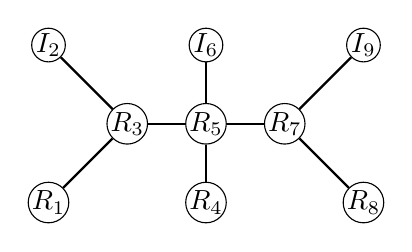
\begin{tikzpicture}[scale=1]
    % Draw a 7,11 network
    % First we draw the vertices
    \foreach \pos/\name in {{(1,1)/R_1}, {(1,3)/I_2}, {(2,2)/R_3}, {(3,1)/R_4}, {(3,2)/R_5}, {(3,3)/I_6}, {(4,2)/R_7}, {(5,1)/R_8}, {(5,3)/I_9}}
        \node[vertex] (\name) at \pos {$\name$};
    
    
    % Connect vertices with edges 
    \foreach \source/ \dest in {R_1/R_3, I_2/R_3, R_3/R_5, R_4/R_5, I_6/R_5, R_5/R_7, R_7/R_8, R_7/I_9}
        \path[edge] (\source) -- (\dest) ;
        
\end{tikzpicture}
\end{center}
\caption{A configuration of the state and the network in which player 1, 3, 4, 5, 7, 8 are Rebels while players 2, 4, 9 are Inerts.}
\label{fig:central_pivotal}
\end{figure}

\begin{figure}


\begin{center}
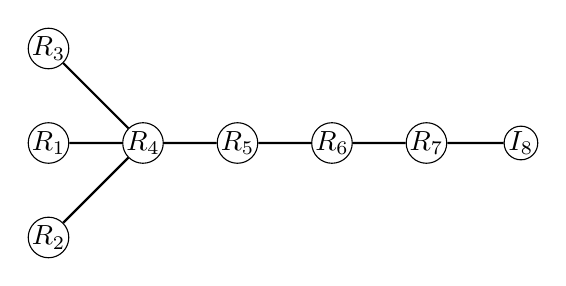
\begin{tikzpicture}[scale=1.2]
    % Draw a 7,11 network
    % First we draw the vertices
    \foreach \pos/\name in {{(2,2)/R_1}, {(2,1)/R_2}, {(2,3)/R_3}, {(3,2)/R_4}, {(4,2)/R_5}, {(5,2)/R_6}, {(6,2)/R_7}, {(7,2)/I_8}}
        \node[vertex] (\name) at \pos {$\name$};
    
    
    % Connect vertices with edges 
    \foreach \source/ \dest in {R_1/R_4, R_2/R_4,R_3/R_4,R_4/R_5, R_5/R_6, R_6/R_7, R_7/I_8}
        \path[edge] (\source) -- (\dest) ;
        
\end{tikzpicture}
\end{center}
\caption{A configuration of the state and the network in which player 1, 2, 3, 4, 5, 6, 7 are Rebels while player 8 is an Inert.}
\label{fig:k-1_pivotal}
\end{figure}

Below is the defined free-rider problem in $\Omicron^t$ .

\begin{definition}
A free-rider problem exists in $\Omicron^t$ if there are multiple $\theta$-pivotal Rebels in $\Omicron^t$.
\end{definition}



The following lemma is crucial. 
%it says that there will be at most two $\theta$-pivotal Rebels in $R^{t}$. Therefore, if there is a free-rider problem, it occurs between two $\theta$-pivotal Rebels. Moreover, if there are two of them, they are neighbors. (... it occurs between two Rebels who are neighbors.)
\begin{lemma}
\label{lemma_at_most_two_nodes}
If the network is acyclic and if $\pi$ has full support on strong connectedness, there are at most two $\theta$-pivotal Rebels in the $t$-block. Moreover, they are neighbors.\footnote{As a remark, Lemma~\ref{lemma_at_most_two_nodes} is not true when the network is cyclic. To see this, consider a 4-player circle when $\theta=(R,R,R,R)$.}
\end{lemma}

Notably,

\begin{lemma}
\label{lemman_pivotals_CK}
If the network is acyclic and if $\pi$ has full support on strong connectedness, when there are two $\theta$-pivotal Rebels $p,p^{'}$ in the $t$-block, then they commonly know that they are $\theta$-pivotal Rebels at the beginning of $t$-block.
\end{lemma}

By Lemma~\ref{lemman_pivotals_CK}, $\theta$-pivotal Rebels in $\Omicron^t$ can identify themselves at the beginning of $\Omicron^t$. This importance cannot be further emphasized. If the free-rider problem occurs in $\Omicron^t$, the strategy can specify that the lowest indexed $\theta$-pivotal Rebel $p$ in the free-rider problem will play $\langle 1 \rangle$, while the other one $p^{'}$ will play $\langle I^t_{p^{'}} \rangle$ \textit{beforehand}. In short, this knowledge is encoded in the belief system of an APEX equilibrium. 

\begin{remark}
It is worth noting that the assumption of acyclic network in Lemma~\ref{lemman_pivotals_CK} is indispensable. Lemma~\ref{lemman_pivotals_CK} does not hold if the network is cyclic as Section~\ref{sec:cyclic} demonstrates it.
\end{remark}

Now I can list the sequences played in $\Omicron^t$ on the path in Table~\ref{Table_msg_RP_path}.

\begin{table}[!htbp]
\caption{The sequences of actions played in $\Omicron^t$ on the path}
\label{Table_msg_RP_path}
\begin{center}
\begin{tabular}{l c}
Rebel $i$ & $i$ plays\\
\hline
\hline
$i\notin R^t$				& $\langle \textbf{all stay} \rangle$  \\
$i\in R^t$ but $i$ is not pivotal	 					 			& $\langle I^t_i \rangle$  \\
$i$ is $k-1$-pivotal	 					 			& $\langle 1 \rangle$  \\
$i$ is $\theta$-pivotal but not in the free-rider problem	 					 			& $\langle 1 \rangle$  \\
$i$ is in the free-rider problem with the lowest index	 					 			& $\langle 1 \rangle$  \\
$i$ is in the free-rider problem without the lowest index	 					 			& $\langle I^t_i \rangle$  \\
\hline
\end{tabular}
\end{center}
\end{table}

%\begin{example}
%\label{ex:cyclic}
%The free-rider problem could become intractable in cyclic networks. Let us consider the configuration in Figure~\ref{fig:cyclic_network}, and suppose $k=4$. 
%\begin{figure}[!h]
%
%\begin{center}
%\begin{tikzpicture}[scale=1]
%    % Draw a 7,11 network
%    % First we draw the vertices
%    \foreach \pos/\name in {{(2,3)/R_1}, {(3,2)/R_2}, {(4.5,2)/R_3}, {(5.5,3)/R_4}, {(3.75,4)/I_5}}
%        \node[vertex] (\name) at \pos {$\name$};
%    
%    
%    % Connect vertices with edges 
%    \foreach \source/ \dest in { R_1/R_2, R_2/R_3, R_3/R_4, R_4/I_5, I_5/R_1}
%        \path[edge] (\source) -- (\dest) ;
%        
%\end{tikzpicture}
%\end{center}
%\caption{A configuration of the state and the network in which player 1, 2, 3, 4 are Rebels while player 5 is an Inert.}
%\label{fig:cyclic_network}
%\end{figure}
%
%Rebels 2 and 3 are $\theta$-pivotal by definition. From the perspective of Rebel 2, the type of player 5 could be Inert. Therefore, Rebel 2 does not know that Rebel 1 is pivotal. Similarly, Rebel 2 does not know that Rebel 3 is pivotal, \textit{even though} player 3 is indeed $\theta$-pivotal. Therefore there is no common knowledge of the free-rider problem at the beginning of $1$-block. 
%
%However, the common knowledge of engaging in a free-rider problem is restored when we cut the edge between player 4 and 5; Rebel 2 knows that he is the only $\theta$-pivotal Rebel.
%\end{example}


\subsection{The equilibrium path in the coordination phase}
\label{sec:eq_cd}
In this section, I discuss the sequences of actions in the coordination phase on the path. The term ``coordination phase in $t$-block'' is shorten by $\Kappa^{t}$. If there is no further mention, all the description in this section is for the APEX equilibrium path \textit{before} the terminal period $T^{\theta}$. 



%The main feature in the periods of coordination is that, whenever a Rebel $i$ is considered inactive starting at some $t$-block, there is no strategy for $i$ to convince all Rebels that $\#[R](\theta)\geq k$ even though $i$ knows it and wants to propagandize it.\footnote{This property might be abstruse at this moment since the equilibrium strategy has not yet been laid out. It however can be proved by tracing the equilibrium path listed in Table~\ref{Table_cd0} to Table~\ref{Table_cdt}.}

To explicitly depict the structure in the coordination phase is tiresome, but it is actually a simple contagion scenario: Rebels jointly decide to terminate or continue their information sharing during this phase. For that, a coordination phase is partitioned into three \textit{divisions}. In the first division, if there is a Rebel has learnt that $\#[R](\theta)<k$, all Rebels will play \textbf{stay} forever after this division; otherwise, they continue to the next one. In the second one, if there is a Rebel has learnt that $\#[R](\theta)\geq k$, a certain portion of Rebels will play \textbf{revolt} forever after this division; otherwise, they continue to the next one. In the third one, if there is a Rebel has learnt that $\#[R](\theta)\geq k$ in previous divisions, all Rebel will play \textbf{revolt} forever after this division; otherwise, they continue to the next phase---a reporting phase.

To fulfil the above contagion argument, create a set of sequences of actions to be played in the equilibrium path so Rebels' belief is updated by observing them. To illustrate these sequence and the equilibrium path, partition a division into \textit{sub-blocks}. I depict the whole partition in the coordination phase below, where $\Box$ represents a sub-block in coordination phase. 

In $\Kappa^1$, 
\[\overbrace{\underbrace{ \Box }_{\text{one sub-block}}}^{\text{$1$-division}} \overbrace{\underbrace{\Box }_{\text{one sub-block}}}^{\text{$2$-division}} \overbrace{\underbrace{\Box \cdot \cdot \cdot \Box}_{\text{$n$ sub-blocks}}}^{\text{$3$-division}}\] 

In $\Kappa^t$, $t\geq 2$,
\[\overbrace{\underbrace{\Box \cdot \cdot \cdot \Box}_{\text{$n$ sub-blocks}}}^{\text{$1$-division}} \overbrace{\underbrace{\Box \cdot \cdot \cdot \Box}_{\text{$t+1$ sub-blocks}} }^{\text{$2$-division}} \overbrace{\underbrace{\Box \cdot \cdot \cdot \Box}_{\text{$n$ sub-blocks}}}^{\text{$3$-division}}\] 


%
%In $\Kappa^1$, 
%\[\overbrace{\underbrace{ \kappa_1 }_{\text{one sub-block}}}^{\text{$1$-division}} \overbrace{\underbrace{\kappa_2 }_{\text{one sub-block}}}^{\text{$2$-division}} \overbrace{\underbrace{\kappa_3 \cdot \cdot \cdot \kappa_{3+n}}_{\text{$n$ sub-blocks}}}^{\text{$3$-division}}\] 
%
%In $\Kappa^t$, $t\geq 2$,
%\[\overbrace{\underbrace{\kappa_1 \cdot \cdot \cdot \kappa_n}_{\text{$n$ sub-blocks}}}^{\text{$1$-division}} \overbrace{\underbrace{\kappa_{n+1} \cdot \cdot \cdot \kappa_{n+t+2}}_{\text{$t+1$ sub-blocks}} }^{\text{$2$-division}} \overbrace{\underbrace{\kappa_{n+t+3} \cdot \cdot \cdot \kappa_{2n+t+3}}_{\text{$n$ sub-blocks}}}^{\text{$3$-division}}\] 
%


%As in the equilibrium construction in Example~\ref{ex:cost_function_talk_solve_fr_Indm}, the behavior in $CD^t$ is dependent on the behavior in $RP^t$ (when $t\geq 1$).

In the $t$-block, denote $\Kappa^t_{u}$ as the $u$-division and $|\Kappa^t_{u} |$ as the length of $\Kappa^t_{u}$. Likewise, denote $\Kappa^t_{u,v}$ as the $v$-th sub-block in $u$-division and $|\Kappa^t_{u,v} |$ as the length of $\Kappa^t_{u,v}$. Let us shorten \textbf{revolt} and \textbf{stay} to \textbf{r} and \textbf{s} receptively. For $v=1,...,n$, let $|\Kappa^t_{u,v}|=n$ if $u=1,2$ and $|\Kappa^t_{u,v}|=1$ if $u=3$. The notations for the sequences of actions on the path are shown in Table~\ref{Table_msg_coordination}.\footnote{Because, in the $3$-division, the length of the sequence of actions is 1, i.e.~playing an action, I dispense notations in the $3$-division for conciseness.}

%When a Rebel $i$ follows the equilibrium path, either $\langle i \rangle$ or $\langle \textbf{all stay} \rangle$ can be observed by him. Notice that a Rebel who is certain $\#[R](\theta)<k$ will always play $\langle \textbf{all stay} \rangle$ in every $\Kappa^t_{u}$ for all $t\geq 0,u=1,2$. Playing $\langle i \rangle$ contrasts with it to represent uncertainty about $\#[R](\theta)$. $\langle i \rangle$ is also crafted to simplify expected payoff calculation: there is at most one \textbf{r} played in $\Kappa^t_u$ for $t\geq 0$, $u=1,2$.    

\begin{table}[!htbp]
\caption{The notations for the sequences of actions in $\Kappa^t_{u,v}$ for $u=1,2$, $v=1,...,n$, on the path}
\label{Table_msg_coordination}
\begin{center}
\begin{tabular}{l c c}
Notations & &The sequences of actions \\
\hline
\hline
$\langle i \rangle$ 				& $\equiv$ 			& $(\overbrace{ \textbf{s},...,\textbf{s},\underbrace{\textbf{r},\textbf{s},...,\textbf{s}}_{i}}^{n} )$  \\
$\langle \textbf{all stay} \rangle$	 					& $\equiv$ 			& $( \overbrace{\textbf{s},...,\textbf{s},{\textbf{s}}}^{n} )$  \\
\hline
\end{tabular}
\end{center}
\end{table}


\subsubsection{The equilibrium behavior on the path in $\Kappa^1$}
Since the $1$-block has a simpler structure, I begin with depicting the equilibrium path in $\Kappa^1$, which is shown in Table~\ref{Table_cd0}. 
%I describe Rebel $i$'s behavior by contingent on whether $i$ has learnt the relevant information. It is not standard but more intuitive, while detailing it in Appendix. Notice that if Rebel $i$ is certain that $\#[R](\theta)<k$, it must be that all Rebels are $i$'s neighbors, by the full support on strong connectedness. Since all Rebels are $i$'s neighbors, they will be also certain $\#[R](\theta)<k$ just after $\Kappa^1_{1}$. 
%Figure~\ref{fig:central_less_k} illustrates this scenario when $3\leq k <n$, in which Rebel 5 is certain $\#[R](\theta)<k$ in $\Kappa^1_1$. Rebel 4 is certain of that right after $\Kappa^1_1$. The idea in Table~\ref{Table_cd0} is as follows. $\Kappa^1_1$ is the periods for a Rebel to advocate the knowledge of $\# [R](\theta)<k$. A Rebel $i$ will initiate coordination to \textbf{s} by playing $\langle \textbf{all stay} \rangle$ if he knows $\# [R](\theta)<k$; otherwise, he will play $\langle i \rangle$. $\Kappa^1_2$ is the periods for a Rebel to advocate the knowledge of $\# [R](\theta)\geq k$. Rebel $i$ will initiate coordination to \textbf{r} by playing $\langle \textbf{all stay} \rangle$ if he knows $\# [R](\theta)\geq k$ and has player $\langle i \rangle$ in the previous division $\Kappa^1_1$; otherwise, he will play $\langle i \rangle$. $\Kappa^t_3$ is used for coordinating to play \textbf{r} or \textbf{s} contagiously.
%
%\begin{figure}
%
%
%\begin{center}
%\begin{tikzpicture}[scale=1]
%    % Draw a 7,11 network
%    % First we draw the vertices
%    \foreach \pos/\name in {{(1,1)/I_1}, {(1,3)/I_2}, {(2,2)/I_3}, {(3,1)/R_4}, {(3,2)/R_5}, {(3,3)/I_6}, {(4,2)/I_7}, {(5,1)/I_8}, {(5,3)/I_9}}
%        \node[vertex] (\name) at \pos {$\name$};
%    
%    
%    % Connect vertices with edges 
%    \foreach \source/ \dest in {I_1/I_3, I_2/I_3, I_3/R_5, R_4/R_5, I_6/R_5, R_5/I_7, I_7/I_8, I_7/I_9}
%        \path[edge] (\source) -- (\dest) ;
%        
%\end{tikzpicture}
%\end{center}
%\caption{A configuration of the state and the network in which player 4, 5 are Rebels while players 1, 2, 3, 6, 7, 8, 9 are Inerts.}
%\label{fig:central_less_k}
%\end{figure}
\begin{table}[!htbp]
\caption{The sequences of actions played in $\Kappa^1$ on the path}
\label{Table_cd0}
\begin{center}
\begin{tabular}{l c}
\multicolumn{2}{c}{The sequences of actions played in $\Kappa^1_{1,1}$ on the path}\\
Rebel $i$ 	 	&  	$i$ plays		 \\
\hline
\hline
$i$ is certain $\#[R](\theta)<k$ 	& 	$\langle \textbf{all stay} \rangle$	\\
$i\notin R^{1}$ and is uncertain $\#[R](\theta)\geq k$	& 	$\langle \textbf{all stay} \rangle$	\\
$i\in R^{1}$ and is uncertain $\#[R](\theta)\geq k$ &  $\langle i \rangle$  \\
$i$ is certain $\#[R](\theta)\geq k$ &  $\langle i \rangle$  \\
\hline
\\
\multicolumn{2}{c}{The sequences of actions played in $\Kappa^1_{2,1}$ on the path}\\
Rebel $i$ 	 	&  	$i$ plays		 \\
\hline
\hline
$i$ is certain $\#[R](\theta)<k$ 	& 	$\langle \textbf{all stay} \rangle$	\\
$i\notin R^{1}$ and is uncertain $\#[R](\theta)\geq k$	& 	$\langle \textbf{all stay} \rangle$	\\
$i\in R^{1}$ and is uncertain $\#[R](\theta)\geq k$ &  $\langle i \rangle$  \\
$i$ is certain $\#[R](\theta)\geq k$ &  $\langle \textbf{all stay} \rangle$  \\
\hline
\\
\multicolumn{2}{c}{The sequences of actions played in $\Kappa^1_{3_v}$, where $v=1,...,n$, on the path}\\
Rebel $i$ 	 	&  	$i$ plays		 \\
\hline
\hline
$i$ is certain $\#[R](\theta)<k$ 	& 	$ \textbf{s} $	\\
$i\notin R^{1}$ and is uncertain $\#[R](\theta)\geq k$	& 	$ \textbf{s} $	\\
$i\in R^{1}$ and is uncertain $\#[R](\theta)\geq k$ &  $ \textbf{s} $  \\
$i$ is certain $\#[R](\theta)\geq k$ &  $ \textbf{r} $  \\
\hline
\end{tabular}
\end{center}
\end{table}

There is a non-trivial construction in the equilibrium path: ``How Rebel $i$ initiates the common knowledge about $\#[R](\theta)\geq k$.'' Rebel $i$ does so by playing $\langle i \rangle$ in $\Kappa^1_{1,1}$ and then play $\langle \textbf{all stay} \rangle$ in $\Kappa^1_{2,1}$. His behavior is thus distinguishable from other kinds of Rebels. His neighbors will know $\#[R](\theta)\geq k$ right after $\Kappa^1_{2,1}$, and then all Rebels will know that by playing \textbf{r} contagiously in $\Kappa^1_{3}$. 

Rebel $i$ will not deviate to play $\langle \textbf{all stay} \rangle$ even though it might be undetectable. This is because the network is acyclic. If $i$ does so, $i$ will be considered as an inactive Rebel at $1$-block afterwards by all of his neighbors. This implies each of $i$'s behavior will be certain that there is no Rebel behind $i$. $i$ then faces the possibility that no Rebels can learn $\#[R](\theta)\geq k$ even if $\#[R](\theta)\geq k$. If this happens, $i$ will only get zero payoff. However, $i$ can surely get payoff of $1$ forever after $\Kappa^1_{2,1}$. Sufficiently high discount factor will deter this deviation. 
%In essence, one major part of proof for Theorem~\ref{thm_main_result} follows the same argument.

%\begin{table}[!htbp]
%\caption{The sequences of actions played in $\Kappa^1_{1}$ on the path}
%\label{Table_cd011}
%\begin{center}
%\begin{tabular}{l c}
%Rebel $i$ 	 	&  	$i$ plays		 \\
%\hline
%\hline
%$i$ is certain $\#[R](\theta)<k$ 	& 	$\langle \textbf{all stay} \rangle$	\\
%$i\notin R^{1}$ and is uncertain $\#[R](\theta)\geq k$	& 	$\langle \textbf{all stay} \rangle$	\\
%$i\in R^{1}$ and is uncertain $\#[R](\theta)\geq k$ &  $\langle i \rangle$  \\
%$i$ is certain $\#[R](\theta)\geq k$ &  $\langle i \rangle$  \\
%\hline
%\end{tabular}
%\end{center}
%\end{table}




%\begin{table}[!htbp]
%\caption{The sequences of actions played in $\Kappa^1_{3}$ on the path}
%\label{Table_cd03v}
%\begin{center}
%\begin{tabular}{l c}
%Rebel $i$ 	 	&  	$i$ plays		 \\
%\hline
%\hline
%$i$ is certain $\#[R](\theta)<k$ 	& 	$\langle \textbf{s} \rangle$	\\
%$i\notin R^{1}$ and is uncertain $\#[R](\theta)\geq k$	& 	$\langle \textbf{s} \rangle$	\\
%$i\in R^{1}$ and is uncertain $\#[R](\theta)\geq k$ &  $\langle \textbf{s} \rangle$  \\
%$i$ is certain $\#[R](\theta)\geq k$ &  $\langle \textbf{r} \rangle$  \\
%\hline
%\end{tabular}
%\end{center}
%\end{table}
%\clearpage

Rebels' belief updating after $\Kappa^1_1$ and $\Kappa^1_2$ on the path are listed in Table~\ref{Table_blf_cd0}. The evolution of information filtrations can be tracked through this table.

\begin{table}[!htbp]
\caption{On the path,  in $\Kappa^1$, the belief of $i$'s neighbor $j$ after observing $i$'s previous actions.}
\label{Table_blf_cd0}
\begin{center}
\begin{tabular}{l  c | c}
 	$i$ plays	  			&	  &  The event on which $j$ assigns probability one  right after $\Kappa^1_{1}$\\
\hline
\hline
In $\Kappa^1_{1}$	&		&		  \\
\hline
  $\langle \textbf{all stay} \rangle$	& &   $i\notin R^1$ if $j\in R^1$ \\
  $\langle \textbf{all stay} \rangle$	&  &  $\#[R](\theta)< k$ if $j\notin R^1$\\
  $\langle i \rangle$	&	&  $i\in R^1$ or $\#[R](\theta)\geq k$    \\
  \hline
  \\
 	$i$ plays	  	&  	  &The event on which $j$ assigns probability one  right after $\Kappa^1_{2}$\\
\hline
\hline
	In $\Kappa^1_{1}$		&			In $\Kappa^1_{2}$	&  \\
\hline
  $\langle \textbf{all stay} \rangle$	&  $\langle \textbf{all stay} \rangle$ &  $i\notin R^1$ if $j\in R^1$ \\
  $\langle \textbf{all stay} \rangle$	&  $\langle \textbf{all stay} \rangle$ &  $\#[R](\theta)< k$ if $j\notin R^1$\\
  $\langle i \rangle$	&	$\langle \textbf{all stay} \rangle$ &  $\#[R](\theta)\geq k$    \\
  $\langle i \rangle$	&	$\langle i \rangle$ &  $i\in R^1$  \\
  \hline
\end{tabular}
\end{center}
\end{table}


%\begin{table}[!htbp]
%\caption{The belief of $j$ after observing his neighbor $i$'s previous actions right after $\Kappa^1_{1}$}
%\label{Table_blf_up_cd01}
%\begin{center}
%\begin{tabular}{l | c}
% 	$i$ plays	  				  &  The event on which $j$ assigns probability one\\
%\hline
%\hline
%In $\Kappa^1_{1}$	&				  \\
%\hline
%  $\langle \textbf{all stay} \rangle$	&    $i\notin R^1$ if $j\in R^1$ \\
%  $\langle \textbf{all stay} \rangle$	&    $\#[R](\theta)< k$ if $j\notin R^1$\\
%  $\langle i \rangle$	&	  $i\in R^1$ or $\#[R](\theta)\geq k$    \\
%  \hline
%\end{tabular}
%\end{center}
%\end{table}
%
%\begin{table}[!htbp]
%\caption{The belief of $j$ after observing his neighbor $i$'s previous actions right after $\Kappa^1_{2}$}
%\label{Table_blf_up_cd02}
%\begin{center}
%\begin{tabular}{l  c | c}
% 	$i$ plays	  	&  	  &The event on which $j$ assigns probability one \\
%\hline
%\hline
%	In $\Kappa^1_{1}$		&			In $\Kappa^1_{2}$	&  \\
%\hline
%  $\langle \textbf{all stay} \rangle$	&  $\langle \textbf{all stay} \rangle$ &  $i\notin R^1$ if $j\in R^1$ \\
%  $\langle \textbf{all stay} \rangle$	&  $\langle \textbf{all stay} \rangle$ &  $\#[R](\theta)< k$ if $j\notin R^1$\\
%  $\langle i \rangle$	&	$\langle \textbf{all stay} \rangle$ &  $\#[R](\theta)\geq k$    \\
%  $\langle i \rangle$	&	$\langle i \rangle$ &  $i\in R^1$  \\
%  \hline
%\end{tabular}
%\end{center}
%\end{table}

%\clearpage

\subsubsection{The equilibrium behavior on the path in $\Kappa^t$ for $t\geq 2$}
Next, I describe the equilibrium behavior on the path in $\Kappa^t$ whenever $t\geq 2$. Players' belief over states will now be contingent on the behavior in $\Omicron^t$ since Rebels share information in $\Omicron^t$. I illustrate players' belief updating in Table~\ref{Table_blf_cdt}. The evolution of information filtrations can be tracked in this table. After that, the in-path strategy contingent on players' belief is introduced in Table~\ref{Table_cdt}. Let us denote $I^{t+1}_{ij}=I^t_i\cap I^t_j$. 

%\clearpage
%\begin{landscape}
\begin{table}[!htbp]
\caption{On the path,  in $\Kappa^t$, the belief of $i$'s neighbor $j$ after observing $i$'s previous actions.}
\label{Table_blf_cdt}
\begin{center}
\begin{tabular}{l l l | c}
%\multicolumn{4}{c}{The belief of $j\in G_i$ after observing $i$'s previous actions right after $\Omicron^t$}\\
 $i$ plays  	&&	&	 The event on which $j$ assigns probability one right after $\Omicron^t$\\
\hline
\hline
 In $\Omicron^t$		&&&					 \\
\hline
$\langle \textbf{all stay} \rangle$  &&&     $i\notin R^t$ and $I^{t+1}_{ji}=I^t_j$ \\
$\langle I^t_{i} \rangle$  &&&     $i\in R^t$ and $I^{t+1}_{ji}=I^t_j\cap I^t_{i}$ \\
$\langle 1 \rangle$  &&& 	  $i$ is pivotal    \\
\hline
%\multicolumn{4}{c}{The belief of $j\in G_i$ after observing $i$'s previous actions right after $\Kappa^t_1$ {contingent} on $\Omicron^t$}\\
\\
 $i$ plays	&&			  & The event on which $j$ assigns probability one right after $\Kappa^t_{1,1}$\\
\hline
\hline
	  In $\Omicron^t$	 	&		In $\Kappa^t_{1,1}$	&		&		  \\
\hline
$\langle \textbf{all stay} \rangle$  & $\langle i \rangle$	&&    $i\notin R^t$ and $I^{t+1}_{ji}=I^t_j$  \\
$\langle I^t_{i} \rangle$  & $\langle \textbf{all stay} \rangle$	&&    $\#[R](\theta)< k$ \\
$\langle I^t_{i} \rangle$  & $\langle i \rangle$	&&   $(\#[R](\theta)\geq k )$ or $(i\in R^t$ and $I^{t+1}_{ji}=I^t_j\cap I^t_{i})$\\
$\langle 1 \rangle$  & $\langle \textbf{all stay} \rangle$	&&	  $\#[R](\theta)< k$    \\
$\langle 1 \rangle$  & $\langle i \rangle$	&&	  $\#[R](\theta)\geq k$  \\
\hline
%\multicolumn{4}{c}{The belief of $j\in G_i$ after observing $i$'s previous actions right after $\Kappa^t_{2}$ {contingent} on $\Omicron^t$, $\Kappa^t_{1}$, and $\Kappa^t_{2}$}\\
\\
 $i$ plays  	&		&  	  &The event on which $j$ assigns probability one right after $\Kappa^t_{2,1}$\\
\hline
\hline
In $\Omicron^t$			&	In $\Kappa^t_{1,1}$			&			In $\Kappa^t_{2,1}$		&   \\
\hline
$\langle \textbf{all stay} \rangle$  & $\langle i \rangle$	&  $\langle \textbf{all stay} \rangle$ &  $i\notin R^t$ and $I^{t+1}_{ji}=I^t_j$  \\
$\langle I^t_{i} \rangle$  & $\langle \textbf{all stay} \rangle$	&  $\langle \textbf{all stay} \rangle$ &  $\#[R](\theta)< k$ \\
$\langle I^t_{i} \rangle$  & $\langle i \rangle$	&  $\langle \textbf{all stay} \rangle$ &  $\#[R](\theta)\geq k$ \\
$\langle I^t_{i} \rangle$  & $\langle i \rangle$	&  $\langle i \rangle$ &  $i\in R^t$ and $I^{t+1}_{ji}=I^t_j\cap I^t_{i}$ \\
$\langle 1 \rangle$  & $\langle \textbf{stay} \rangle$	&	$\langle \textbf{all stay} \rangle$ &  $\#[R](\theta)< k$    \\
$\langle 1 \rangle$  & $\langle i \rangle$	&	$\langle \textbf{all stay} \rangle$ &  $\#[R](\theta)\geq k$  \\
  \hline
\end{tabular}
\end{center}
\end{table}
%\end{landscape}

%\clearpage

%\begin{table}[!htbp]
%\caption{The belief of $j$ after observing his neighbor $i$'s previous actions right after $\Omicron^t$ }
%\label{Table_blf_up_rpt}
%\begin{center}
%\begin{tabular}{l | c}
% $i$ plays  		&	 The event on which $j$ assigns probability one \\
%\hline
%\hline
% In $\Omicron^t$		&					 \\
%\hline
%$\langle \textbf{all stay} \rangle$  &     $i\notin R^t$ and $I^{t+1}_{ji}=I^t_j$ \\
%$\langle I^t_{i} \rangle$  &     $i\in R^t$ and $I^{t+1}_{ji}=I^t_j\cap I^t_{i}$ \\
%$\langle 1 \rangle$  & 	  $i$ is pivotal    \\
%  \hline
%\end{tabular}
%\end{center}
%\end{table}
%
%
%
%\begin{table}[!htbp]
%\caption{The belief of $j$ after observing his neighbor $i$'s previous actions right after $\Kappa^t_1$ {contingent} on $\Omicron^t$ }
%\label{Table_blf_up_cdt1}
%\begin{center}
%\begin{tabular}{l  l | c}
% $i$ plays	&			  & The event on which $j$ assigns probability one \\
%\hline
%\hline
%	  In $\Omicron^t$	 	&		In $\Kappa^t_{1,1}$	&				  \\
%\hline
%$\langle \textbf{all stay} \rangle$  & $\langle i \rangle$	&    $i\notin R^t$ and $I^{t+1}_{ji}=I^t_j$  \\
%$\langle I^t_{i} \rangle$  & $\langle \textbf{all stay} \rangle$	&    $\#[R](\theta)< k$ \\
%$\langle I^t_{i} \rangle$  & $\langle i \rangle$	&   $\#[R](\theta)\geq k$, or $i\in R^t$ and $I^{t+1}_{ji}=I^t_j\cap I^t_{i}$  \\
%$\langle 1 \rangle$  & $\langle \textbf{all stay} \rangle$	&	  $\#[R](\theta)< k$    \\
%$\langle 1 \rangle$  & $\langle i \rangle$	&	  $\#[R](\theta)\geq k$  \\
%  \hline
%\end{tabular}
%\end{center}
%\end{table}
%
%\begin{table}[!htbp]
%\caption{The belief of $j$ after observing his neighbor $i$'s previous actions right after $\Kappa^t_{2}$ {contingent} on $\Omicron^t$, $\Kappa^t_{1}$, and $\Kappa^t_{2}$ }
%\label{Table_blf_up_cdt2}
%\begin{center}
%\begin{tabular}{l  l l | c}
% $i$ plays  	&		&  	  & The event on which $j$ assigns probability one \\
%\hline
%\hline
%In $\Omicron^t$			&	In $\Kappa^t_{1,1}$			&			In $\Kappa^t_{2,1}$		&   \\
%\hline
%$\langle \textbf{all stay} \rangle$  & $\langle i \rangle$	&  $\langle \textbf{all stay} \rangle$ &  $i\notin R^t$ and $I^{t+1}_{ji}=I^t_j$  \\
%$\langle I^t_{i} \rangle$  & $\langle \textbf{all stay} \rangle$	&  $\langle \textbf{all stay} \rangle$ &  $\#[R](\theta)< k$ \\
%$\langle I^t_{i} \rangle$  & $\langle i \rangle$	&  $\langle \textbf{all stay} \rangle$ &  $\#[R](\theta)\geq k$ \\
%$\langle I^t_{i} \rangle$  & $\langle i \rangle$	&  $\langle i \rangle$ &  $i\in R^t$ and $I^{t+1}_{ji}=I^t_j\cap I^t_{i}$ \\
%$\langle 1 \rangle$  & $\langle \textbf{stay} \rangle$	&	$\langle \textbf{all stay} \rangle$ &  $\#[R](\theta)< k$    \\
%$\langle 1 \rangle$  & $\langle i \rangle$	&	$\langle \textbf{all stay} \rangle$ &  $\#[R](\theta)\geq k$  \\
%  \hline
%\end{tabular}
%\end{center}
%\end{table}

%\clearpage

\begin{table}[!htbp]
\caption{The sequences of actions played in $\Kappa^t$, $t\geq 2$ on the path}
\label{Table_cdt}
\begin{center}
\begin{tabular}{l c}
\multicolumn{2}{c}{The sequences of actions played in $\Kappa^t_{1,v}$ for $t\geq 2$ and for $v=1,2,...,n$ on the path}\\
Rebel $i$ 	 	&  	$i$ plays		 \\
\hline
\hline
$i$ is certain $\#[R](\theta)<k$ 	& 	$\langle \textbf{all stay} \rangle$	\\
$i\notin R^{t}$ and is uncertain $\#[R](\theta)\geq k$	& 	$\langle i \rangle$	\\
$i\in R^{t}$ and is uncertain $\#[R](\theta)\geq k$ &  $\langle i \rangle$  \\
$i$ is certain $\#[R](\theta)\geq k$ &  $\langle i \rangle$  \\
\hline
\\
\multicolumn{2}{c}{The sequences of actions played in $\Kappa^t_{2,v}$ for $t\geq 2$ for $v=1$ on the path}\\
Rebel $i$ 	 	&  	$i$ plays		 \\
\hline
\hline
$i$ is certain that $\#[R](\theta)<k$ 	& 	$\langle \textbf{all stay} \rangle$	\\
$i\notin R^{t}$ and is uncertain $\#[R](\theta)\geq k$	& 	$\langle \textbf{all stay} \rangle$	\\
$i\in R^{t}$ and is uncertain $\#[R](\theta)\geq k$ &  $\langle i \rangle$  \\
$i$ is certain that $\#[R](\theta)\geq k$ &  $\langle \textbf{all stay} \rangle$  \\
\hline
\\
\multicolumn{2}{c}{The sequences of actions played in $\Kappa^t_{2,v}$ for $t\geq 2$ for $v=2,...,t+1$ on the path}\\
Rebel $i$ 	 	&  	$i$ plays		 \\
\hline
\hline
$i$ is certain that $\#[R](\theta)<k$ 	& 	$\langle \textbf{all stay} \rangle$	\\
$i\notin R^{t}$ and is uncertain $\#[R](\theta)\geq k$	& 	$\langle \textbf{all stay} \rangle$	\\
$i\in R^{t}$ and is uncertain $\#[R](\theta)\geq k$ &  $\langle \textbf{all stay} \rangle$  \\
$i$ is certain that $\#[R](\theta)\geq k$ &  $\langle i \rangle$  \\
\hline
\\
\multicolumn{2}{c}{The sequences of actions played in $\Kappa^t_{3}$ for $t\geq 2$ on the path}\\
Rebel $i$ 	 	&  	$i$ plays		 \\
\hline
\hline
$i$ is certain that $\#[R](\theta)<k$ 	& 	$\textbf{s}$	\\
$i\notin R^{1}$ and is uncertain $\#[R](\theta)\geq k$	& 	$ \textbf{s} $	\\
$i\in R^{1}$ and is uncertain $\#[R](\theta)\geq k$ &  $ \textbf{s} $  \\
$i$ is certain that $\#[R](\theta)\geq k$ &  $ \textbf{r} $  \\
\hline
\end{tabular}
\end{center}
\end{table}


The delicate part in $\Kappa^t$ is how a pivotal Rebel $p$ propagandizes the relevant information. $p$ does so by playing $\langle \textbf{all stay} \rangle$ in $\Kappa^{t}_{1,1}$ in the case of $\#[R](\theta)< k$, while playing $\langle p \rangle$ in the case of $\#[R](\theta)\geq k$. Notice that playing $\langle \textbf{all stay} \rangle$ in $\Kappa^{t}_{1,1}$ by $p$ will immediately inform $p$'s neighbors that $\#[R](\theta)< k$. On the contrary, playing sequence other than $\langle \textbf{all stay} \rangle$ has not yet revealed $\#[R](\theta)\geq k$ since that might be played by other non-pivotal Rebels. 

In $\Kappa^{t}_{2,1}$, $p$ reveals $\#[R](\theta)\geq k$ by playing $\langle \textbf{all stay} \rangle$, which is a costless sequence of actions. It might not seem intuitive at first sight, but it effectively prevents a potential free-rider problem: there are two pivotal Rebels, say $p$ and $p^{'}$, who have already known $\#[R](\theta)\geq k$ in $\Kappa^t$. If initiating the common knowledge about $\#[R](\theta)\geq k$ incurs negative payoff, $p$ or $p^{'}$ will have the incentive (again!) to let the other one initiate it. Playing $\langle \textbf{all stay} \rangle$ in $\Kappa^t_{2,1}$ proudly becomes the initiation sequence by its cheapness.

The remaining argument is why other non-pivotal Rebels, say $i$, do not mimic the pivotal Rebels' behavior to play $\langle 1 \rangle$ in $\Omicron^t$. If $i$ plays $\langle 1 \rangle$, all Rebels will learn the relevant information right after $\Kappa^t_2$ based on the belief updating on the path. It implies that the beginning of $t+1$-block is the terminal period. He will not learn the relevant information after that because the belief updating will be also terminated. However, he is still uncertain whether he can learn the relevant information in $\Omicron^t$ since he is not pivotal. Since that the ex-post efficient outcome gives him the maximum payoff at every $\theta$, and that he will learn the relevant information eventually on the equilibrium path, he prefers not to deviate given that the discount factor is high enough.\footnote{Since $R^t$ Rebels share information on the equilibrium path, by Theorem~\ref{lemma_empty}, the belief updating in Table~\ref{Table_blf_cd0}, Table~\ref{Table_blf_cdt}, and the in-path behavior in Table~\ref{Table_cdt}, the relevant information is learnt by every Rebel eventually on the path.} 
%The proof of Theorem~\ref{thm_main_result} heavily depends on arguments of this kind.

%The idea in Table~\ref{Table_cdt} is as follows. 
%$\Kappa^t_1$ is the periods for a Rebel to advocate the knowledge of $\# [R](\theta)<k$. A Rebel $i$ will initiate coordination to \textbf{s} by playing $\langle \textbf{all stay} \rangle$ in $\Kappa^t_{1,1}$ if he knows $\# [R](\theta)<k$; otherwise, he will play $\langle i \rangle$. $\Kappa^t_2$ is the periods for a Rebel to advocate the knowledge of $\# [R](\theta)\geq k$. A Rebel $i$ will initiate coordination to \textbf{r} by playing $\langle \textbf{all stay} \rangle$ in $\Kappa^t_{2,1}$ if he knows $\# [R](\theta)\geq k$ and has played $\langle 1 \rangle$ in the previous periods $\Omicron^t$; otherwise, he will play $\langle i \rangle$. $\Kappa^t_3$ is used for coordinating to play \textbf{r} or \textbf{s} contagiously.




%\begin{table}[!htbp]
%\caption{The sequences of actions played in $\Kappa^t_{2,v}$ for $t\geq 1$ for $v=1$ on the path}
%\label{Table_cdt21}
%\begin{center}
%\begin{tabular}{l c}
%Rebel $i$ 	 	&  	$i$ plays		 \\
%\hline
%\hline
%$i$ is certain that $\#[R](\theta)<k$ 	& 	$\langle \textbf{all stay} \rangle$	\\
%$i\notin R^{t}$ and is uncertain $\#[R](\theta)\geq k$	& 	$\langle \textbf{all stay} \rangle$	\\
%$i\in R^{t}$ and is uncertain $\#[R](\theta)\geq k$ &  $\langle i \rangle$  \\
%$i$ is certain that $\#[R](\theta)\geq k$ &  $\langle \textbf{all stay} \rangle$  \\
%\hline
%\end{tabular}
%\end{center}
%\end{table}


%\begin{table}[!htbp]
%\caption{The sequences of actions played in $\Kappa^t_{2,v}$ for $t\geq 1$ for $v=2,...,t+1$ on the path}
%\label{Table_cdt2t}
%\begin{center}
%\begin{tabular}{l c}
%Rebel $i$ 	 	&  	$i$ plays		 \\
%\hline
%\hline
%$i$ is certain that $\#[R](\theta)<k$ 	& 	$\langle \textbf{all stay} \rangle$	\\
%$i\notin R^{t}$ and is uncertain $\#[R](\theta)\geq k$	& 	$\langle \textbf{all stay} \rangle$	\\
%$i\in R^{t}$ and is uncertain $\#[R](\theta)\geq k$ &  $\langle \textbf{all stay} \rangle$  \\
%$i$ is certain that $\#[R](\theta)\geq k$ &  $\langle i \rangle$  \\
%\hline
%\end{tabular}
%\end{center}
%\end{table}


%\begin{table}[!htbp]
%\caption{The sequences of actions played in $\Kappa^t_{3}$ for $t\geq 1$ on the path}
%\label{Table_cdt3v}
%\begin{center}
%\begin{tabular}{l c}
%Rebel $i$ 	 	&  	$i$ plays		 \\
%\hline
%\hline
%$i$ is certain that $\#[R](\theta)<k$ 	& 	$\textbf{s}$	\\
%$i\notin R^{1}$ and is uncertain $\#[R](\theta)\geq k$	& 	$ \textbf{s} $	\\
%$i\in R^{1}$ and is uncertain $\#[R](\theta)\geq k$ &  $ \textbf{s} $  \\
%$i$ is certain that $\#[R](\theta)\geq k$ &  $ \textbf{r} $  \\
%\hline
%\end{tabular}
%\end{center}
%\end{table}
%\clearpage






%
%
%
%\begin{example} This example demonstrates the learning process on the equilibrium path. Let us take the configuration in Figure~\ref{fig:T-round-6}.
%
%Let $k=6$. Players have their prime numbers as $(x_1,x_2,...,x_8)=(3,5,7,11,13,17,19,23)$.
%
%At $\Kappa^1_{1}$, Rebels 1, 2, 6, and 8 play $\langle \textbf{all stay} \rangle$; Rebels 4 and 5 play $\langle 4 \rangle$ and $\langle 5 \rangle$ respectively. 
%
%At $\Kappa^1_{2}$, Rebels 1, 2, 6, and 8 play $\langle \textbf{all stay} \rangle$; Rebels 4 and 5 play $\langle 4 \rangle$ and $\langle 5 \rangle$ respectively.
%
%At $\Kappa^1_{3,v}$, for $v=1,..,n$, all Rebels play $\textbf{s} $. 
%
%right after $\Kappa^1_{3}$, all Rebels are uncertain $\# [R](\theta)\geq k$.
%
%At $\Omicron^1$, $|\Omicron^1|=111546435$. Rebels 1, 2, 6, and 8 play 
%\[\langle \textbf{all stay} \rangle=\langle \overbrace{\textbf{s},...,\textbf{s}}^{111546435} \rangle.\] Rebel 4 plays 
%\[\langle 1 \rangle=\langle \overbrace{\textbf{s},...,\textbf{s},\textbf{r}}^{111546435} \rangle.\] Rebel 5 plays 
%\[\langle \{4,5,6,8\} \rangle=\langle \overbrace{\textbf{s},...,\textbf{s},\underbrace{\textbf{r},\textbf{s},...,\textbf{s}}_{55913}}^{111546435} \rangle.\] right after $\Omicron^1$, Rebel 4 is certain $\# [R](\theta)\geq k$, while Rebels 1,2,5,6,8 are not.
%
%At $\Kappa^1_{1,v}$ for $v=1,...,n$, Rebel $i$ plays $\langle i \rangle$. Rebels 1,2,4,5 are certain $\# [R](\theta)\geq k$, while the others are not.
%
%At $\Kappa^1_{2,1}$, Rebels 6 and 8 play $\langle 6 \rangle$ and $\langle 8 \rangle$ respectively. Rebels 1,2,4,5 play $\langle \textbf{all stay} \rangle$. right after $\Kappa^1_{2,1}$, Rebels 6 and 8 also know $\# [R](\theta)\geq k$.
%
%At $\Kappa^1_{2,2}$, all Rebels play $\langle \textbf{all stay} \rangle$.
%
%At $\Kappa^1_{2,v}$ for $v=1,...,n$, all Rebels play $\textbf{r}$. 
%
%After $\Kappa^1_{2,n}$, all Rebels play \textbf{r} forever. 
%
%
%
%\end{example}






\section{Discussion}
\label{sec:varies}
%
%


%\subsubsection{Variation: Rebels with different levels of efforts}
%
%We may also consider a model in which players contribute different levels of efforts to a collective action. Let the set of states of nature be $\hat{\Theta}=\Theta \times \Xi$, where $\Theta=\{Rebel,Inert\}^n$ and $\Xi=\{1,2,...,k\}^n$. Let $\hat{\theta}=(\theta,e)$ be a state of nature. After $\hat{\theta}$ is realized, a player $i$ will hold an endowment $e_i$, where $e_i\in \{1,2,...,k\}$. The payoff structure is modified as the following.
%\begin{enumerate}
%\item $u_{Rebel_i}(a_{Rebel_i},a_{-\theta_i})=b_i$ if $a_{Rebel_i}=\textbf{revolt}$ and $\sum_{j:a_{\theta_j}=\textbf{revolt}}e_j\geq k$
%\item $u_{Rebel_i}(a_{Rebel_i},a_{-\theta_i})=-e_i$ if $a_{Rebel_i}=\textbf{revolt}$ and $\sum_{j:a_{\theta_j}=\textbf{revolt}}e_j< k$
%\item $u_{Rebel_i}(a_{Rebel_i},a_{-\theta_i})=0$ if $a_{Rebel_i}=\textbf{stay}$
%\item $u_{Inert_i}(a_{Inert_i},a_{-\theta_i})=1$ if $a_{Inert_i}=\textbf{stay}$
%\end{enumerate}
%
%
%
%After $\hat{\theta}$ is realized, players repeatedly play the above game in a network $G$. To see that the strategies constructed in previous section is still an equilibrium, we can transform $(G,\hat{\Theta})$ to $(G^{'},\hat{\Theta}^{'})$, where each player $i$ is attached with $\#e_i$ different players in $G^{'}$, and $\hat{\Theta}^{'}=\Theta\times \{1\}^{n}$. 
%
%


\subsection{Payoff as signals}
The hidden payoff assumption can be relaxed without changing the main result. One may consider a situation in which the stage payoff depends not only on players' joint efforts but also on a random shock, say the weather. To fix the idea, there is a public signal $y\in \{r,s\}$ generated according to the action profile. Let a Rebel's payoff function be $u_{R}(a_{R},y)$ such that $u_{R}(\textbf{stay},r)=u_{R}(\textbf{stay},s)=u_0$. $y$ is drawn from the distribution of 
\begin{eqnarray*}
p_{rr} &=& \mathrm {Pr}(y=r|\#\{j:a_j\textbf{revolt}\}\geq k) \\
p_{sr}=1-p_{rr} &=& \mathrm {Pr}(y=s|\#\{j:a_j\textbf{revolt}\}\geq k) \\
p_{ss} &=& \mathrm {Pr}(y=s|\#\{j:a_j\textbf{revolt}\}< k) \\
p_{rs}=1-p_{ss} &=& \mathrm {Pr}(y=r|\#\{j:a_j\textbf{revolt}\}< k) \\
\end{eqnarray*}
such that
\begin{equation*}
p_{rr}u_{R}(\textbf{revolt}, r)+p_{sr}u_{R}(\textbf{revolt}, s)>u_0>p_{rr}u_{R}(\textbf{revolt}, r)+p_{ss}u_{R}(\textbf{revolt}, s),
\end{equation*}
and
\begin{equation*}
0\leq p_{rs}\leq 1,0\leq p_{ss}\leq 1.
\end{equation*}

The APEX equilibrium constructed for Theorem~\ref{thm_main_result} is still a one in this scenario. Note that in that APEX equilibrium path, at most one \textbf{revolt} can occur at every period before some Rebel plays $\langle 1 \rangle$. This implies that the signal $y$ is completely uninformative before some Rebel plays $\langle 1 \rangle$. If a Rebel $i$ deviates to play $\langle 1 \rangle$ in $\Omicron^t$ at some $t$ in the hope gathering information from $y$, he will not learn the relevant information after $\Omicron^t$ since the terminal period will come right after $t$-block. He will, however, learn the relevant information and play the ex-post efficient outcome if he is on the path, and hence he will not deviate.

%If $p_{rr}$ or $p_{ss}=1$, an APEX equilibrium can be easily constructed: all Rebels play \textbf{revolt} in the first period and then keep playing \textbf{revolt} or \textbf{stay} contingent on the signals $y=r$ or $y=s$ respectively.

\subsection{Cyclic networks}
\label{sec:cyclic}


Scenarios in cyclic networks substantially differ from the acyclic counterpart. The free-rider problem could become intractable in cyclic networks. Let us consider the configuration in Figure~\ref{fig:cyclic_network}, and suppose $k=4$.

\begin{figure}[!h]

\begin{center}
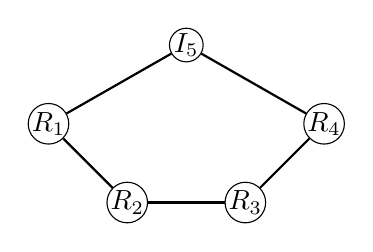
\begin{tikzpicture}[scale=1]
    % Draw a 7,11 network
    % First we draw the vertices
    \foreach \pos/\name in {{(2,3)/R_1}, {(3,2)/R_2}, {(4.5,2)/R_3}, {(5.5,3)/R_4}, {(3.75,4)/I_5}}
        \node[vertex] (\name) at \pos {$\name$};
    
    
    % Connect vertices with edges 
    \foreach \source/ \dest in { R_1/R_2, R_2/R_3, R_3/R_4, R_4/I_5, I_5/R_1}
        \path[edge] (\source) -- (\dest) ;
        
\end{tikzpicture}
\end{center}
\caption{A configuration of the state and the network in which player 1, 2, 3, 4 are Rebels while player 5 is an Inert.}
\label{fig:cyclic_network}
\end{figure}

In Figure~\ref{fig:cyclic_network}, Rebels 2 and 3 are $\theta$-pivotal by definition. From the perspective of Rebel 2, the type of player 5 could be Inert. Therefore, Rebel 2 does not know that Rebel 1 is pivotal. Similarly, Rebel 2 does not know that Rebel 3 is pivotal, \textit{even though} player 3 is indeed $\theta$-pivotal. Therefore there is no common knowledge of the free-rider problem at the beginning of $1$-block. 

However, the common knowledge of engaging in a free-rider problem is restored when we cut the edge between player 4 and 5; Rebel 2 knows that he is the only $\theta$-pivotal Rebel.

I leave a conjecture in this paper and end this section.

\begin{conjecture}
For any $n$-person repeated $k$-Threshold game with parameter $ k < n$ played in any network,
if $\pi$ has full support on strong connectedness, then there exists a $\delta^{*}\in (0,1)$ such that an APEX equilibrium exists whenever $\delta>\delta^{*}$.
\end{conjecture}
%
%
%

\section{Conclusion}
\label{sec:con}

I model a coordination game and illustrate the learning processes generated by strategies in a (weak) sequential equilibrium to answer the question proposed in the beginning: what kind of networks can conduct coordination in a collective action with information barrier. In the equilibrium, players transmit the relevant information by encoding such information by their actions as time goes by. Since there might be an negative expected payoff in coding information, the potential free-rider problems might occur to impede the learning process. My result show that if the network is acyclic, players can always learn the underlying relevant information and conduct the coordination only by actions. In cyclic networks, however, what kinds of equilibrium strategies can lead to learning the relevant information still remains to be answered.


The construction of the communication protocol by actions exploits the assumption of the common knowledge of the network and the finite type space. Since the relevant information has been parametrized as a threshold in the stage game, players can acquire this information by jointly incrementally reporting their own private information period by period. The major punishment to deter deviation is then the joint shifting to play that same action as the stopping to update information. The threshold game thus seems a potential model in proofing that a communication protocol by actions not only leads a learning process but also constitutes an equilibrium to reveal the relevant information in finite time.

Existing literatures in political science and sociology have recognized the importance of social network in influencing individual's behavior in participating social movements ( \citep{Passy2003}\citep{McAdam2003}\citep{Siegel2009}). This paper views networks as routes for communication in which rational individuals initially have local information but they can influence nearby individuals by taking actions. Such influence may take long time to travel across individuals and the whole process incurs inefficient outcomes in many periods. A characterization in the speed of information transmission across a network is not answered here, although it is an important topic in investigating the most efficient way to let the information be spread. This question would remain for the future research.



\bibliographystyle{abbrvnat}	% (uses file "plain.bst")
\bibliography{bigref}		% expects file "myrefs.bib"


\appendix
\section{Appendix}
\subsection{The APEX equilibrium for Theorem~\ref{thm_main_result}}
\subsubsection{Equilibrium path}
\label{sec:equilibrium_path}
By definition of information hierarchy, 
\begin{eqnarray*}
I^t_i & = & \bigcup_{k_1\in G_i}\bigcup_{k_2\in G_{k_0}}...\bigcup_{k_{t}\in G_{k_{t-1}}}I^1_{k_{t}}\\
&= & \{j\in [R](\theta): \text{$\exists$ a path $(i,k_1...k_{l},j)$ s.t.~$0\leq l\leq t-1$ and $\theta_i=\theta_{k_1}=...=\theta_{k_l}=R$}\}
\end{eqnarray*}
Let us define several notions.
\begin{definition}[Extended tree by $I^t_i$]
\label{def:ext_tree}
\begin{eqnarray*}
X^t_i & \equiv &  \{j\in N: \\
	& & \text{$\exists$ a path $(i,k_1...k_{l},k_{l+1})$ s.t.~$k_{l+1}=j$, $l\geq t-1$, $\{i,k_1,...,k_{t}\}\subset I^t_i$}\}\cup I^t_i
\end{eqnarray*}
\end{definition}
$X^t_i $ is the set of all possible Rebels in $G$ given information $I^t_i$. 

\begin{definition}[The tree rooted in $i$ and spanning in the direction toward $j$]
\[TR_{ij}\equiv \{v\in N:\text{there is a path from $i$ to $v$ through $j$, $j\in G_i$}\}\cup\{i,j\}\]
\end{definition}


\begin{definition}[Extended vertices outside $I^t_i$ in $TR_{ij}$]
\[Y^t_{ij}\equiv TR_{ij}\cap(X^t_i\setminus I^t_i)\]
\end{definition}


\begin{definition}[$i$'s capable neighbors by $I^t_i$]
\[D^t_{i}\equiv \{j\in G_i: Y^t_{ij}\neq \emptyset\}\]
\end{definition}




\begin{definition}[Finite register machine]
A finite register machine for $i$ consists of finite registers $\Sigma$. A register is a tuple \[(\Omega, \times_{G_i}A_R,f,\lambda),\] in which $\Omega$ are sets of events induced by $H_i$. $\times_{G_i}A_R$ is the sets of input. $f:\Omega\rightarrow A_{R}$ assigns an action to each event. $\lambda: \Omega\times \times_{G_i}A_R \rightarrow \Sigma$ is the transition function. There is a set of initial registers. 
\end{definition}

$i$'s register specifies $i$'s action according his information at a certain period but does not characterize $i$'s information transition. The register machine here is more like the \textit{switch function} instead of the finite automata. The information of $i$ up to period $s$ is $P_i(\theta)\times \{h^s_{G_i}\}\times H^s_{N\setminus G_i}$ characterized in Section~\ref{sec:model}. 

\begin{definition}[$m$-register in $t$-block]
A $m$-register in a (sub)block or a division is the register in the $m$-th period in that (sub)block or division.
\end{definition}

To shorten the notation, denote $m\dashv\Gamma$ as the $m$-register in the (sub)block or division $\Gamma$.

\begin{definition}[Terminal \textbf{r}]
The terminal \textbf{r} is a register such that the image of $f$ is $\{\textbf{revolt}\}$ and the image of $\lambda$ is a singleton containing itself. 
\end{definition}

\begin{definition}[Terminal \textbf{s}]
The terminal \textbf{s} is a register such that the image of $f$ is $\{\textbf{stay}\}$ and the image of $\lambda$ is a singleton containing itself. 
\end{definition}

The equilibrium will be represented as a {finite register machine}. Moreover, though players act as if acting a whole sequence, they in fact act period by period. For convenience, for any finite sequence of action $\langle \rangle$, denote $\langle \rangle_m$ as the $m$-th (counting from the beginning) component in $\langle \rangle$, and denote $\langle \rangle(m)$ as the prefix of $\langle \rangle$ with length $m$. Let us also shorten action \textbf{revolt} to be \textbf{r} and \textbf{stay} to be \textbf{s}. 

\paragraph{Initial registers}
%\noindent{\textbf{Initial registers}
The initial register for each Rebel is $1\dashv\Kappa^1_1$, which is defined in the next section.
\paragraph{Registers in $\Kappa^1$}
%\noindent{\textbf{Equilibrium path in $\Kappa^1$}}

\begin{landscape}
\begin{table}[!htbp]
\caption{The $m\dashv\Kappa^1_{1}$ on the path}
\label{table:eqm_path_k01}
\begin{center}
\begin{tabular}{c c | c | c | c }
\multicolumn{5}{c}{$1\leq m \leq |\Kappa^1_1|-1$}\\
$\omega_i$ 	 & 	   &	$f(\omega_i)$  &	$a_{G_i}$ & $\lambda(\omega_i,a_{G_i})$ \\
\hline
\hline
$\# X^1_i<k$  	& 	 &$\langle \textbf{all stay} \rangle_m$ &	& terminal \textbf{s}\\
$i\notin R^1$, $\# X^1_i\geq k$, $I^1_i< k$  	&  &$\langle \textbf{all stay} \rangle_m$ & 	& $m+1\dashv\Kappa^1_{1}$\\
$i\in R^1$, $\# X^1_i\geq k$, $I^1_i< k$  	& 	 &$\langle i \rangle_m$	&  & $m+1\dashv \Kappa^1_{1}$\\
$i\in R^1$, $\# X^1_i\geq k$, $I^1_i\geq k$  	& 	 &$\langle i \rangle_m$	&  & $m+1\dashv \Kappa^1_{1}$\\
\hline
\\
\multicolumn{5}{c}{$m=|\Kappa^1_1|$}\\
$\omega_i$ 	 & 	   &	$f(\omega_i)$  &	$a_{G_i}$ & $\lambda(\omega_i,a_{G_i})$ \\
\hline
\hline
$\# X^1_i<k$  	& 	& $\langle \textbf{all stay} \rangle_m$	&     & terminal \textbf{s}\\
$i\notin R^1$, $\# X^1_i\geq k$, $I^1_i< k$   	& all $j$ play $\langle \textbf{all stay} \rangle(m-1)$ & $\langle \textbf{all stay} \rangle_m$	 & all $j$ play \textbf{s} & terminal \textbf{s}\\
$i\notin R^1$, $\# X^1_i\geq k$, $I^1_i< k$   	& $\exists j$ plays $\langle j \rangle(m-1)$ & $\langle \textbf{all stay} \rangle_m$	& such $j$ plays $\langle j \rangle_m$  & $1\dashv \Kappa^1_2$\\
$i\in R^1$, $\# X^1_i\geq k$, $I^1_i< k$   	& 	& $\langle i \rangle_m$	&& $1\dashv \Kappa^1_2$ \\
$i\in R^1$, $\# X^1_i\geq k$, $I^1_i\geq k$  	& 	& $\langle i \rangle_m$ &	& $1\dashv \Kappa^1_2$ \\
\hline
\end{tabular}
\end{center}
\end{table}



\end{landscape}

\begin{landscape}
\begin{table}[!htbp]
\caption{The $m\dashv\Kappa^1_{2}$ on the path}
\label{table:eqm_path_k02}
\begin{center}
\begin{tabular}{c c | c | c | c}
\multicolumn{5}{c}{$1\leq m < |\Kappa^1_2|$}\\
$\omega_i$ 	 & 	   &	$f(\omega_i)$  &	$a_{G_i}$ & $\lambda(\omega_i,a_{G_i})$ \\
\hline
\hline
$i\notin R^1$  	& & $\langle \textbf{all stay} \rangle_m$	&    & $m+1\dashv \Kappa^1_{2}$\\
$i\in R^1$, $I^1_i< k$  	& $\exists j\in G_i$, $j$ plays $<j>_j=s$	& $\langle \textbf{all stay} \rangle_m$	& 	& $m+1\dashv \Kappa^1_{2}$\\
$i\in R^1$, $I^1_i< k$  	& $\forall j\in G_i$, $j$ plays $<j>_j=r$ 	& $\langle i \rangle_m$	& 	& $m+1\dashv \Kappa^1_{2}$\\
$i\in R^1$, $I^1_i\geq k$  	& 	& $\langle \textbf{all stay} \rangle_m$	&	& $m+1\dashv \Kappa^1_{2}$\\
\hline
\\
\multicolumn{5}{c}{$m= |\Kappa^1_2|$}\\
$\omega_i$ 	 & 	   &	$f(\omega_i)$  &	$a_{G_i}$ & $\lambda(\omega_i,a_{G_i})$ \\
\hline
\hline
$i\notin R^1$  	& $\forall j\in G_i$, $j$ plays $\langle j \rangle(m-1)$    & $\langle \textbf{all stay} \rangle_m$	& $\forall j\in G_i$, $j$ plays $\langle j \rangle_m$	& $1\dashv \Kappa^1_{3}$\\
$i\notin R^1$  	& $\exists j\in G_i$, $j$ plays $\langle \textbf{all stay} \rangle(m-1)$   & $\langle \textbf{all stay} \rangle_m$	& such $j$ plays $\langle \textbf{all stay} \rangle_m$	& terminal \textbf{r}\\
$i\in R^1$, $I^1_i< k$   	& $\forall j\in G_i$, $j$ play $\langle j \rangle(m-1)$ 	& $\langle i \rangle_m$	&  $\forall j\in G_i$, $j$ plays $\langle j \rangle_m$	& $1\dashv \Kappa^1_{3}$ \\
$i\in R^1$, $I^1_i< k$   	&  $\exists j\in G_i$, $j$ plays $\langle \textbf{all stay} \rangle(m-1)$ 	& $\langle i \rangle_m$	& such $j$ plays $\langle \textbf{all stay} \rangle_m$	&  terminal \textbf{r}\\
$i\in R^t$, $I^1_i\geq k$  	& 	& $\langle \textbf{all stay} \rangle_m$	& 	& terminal \textbf{r} \\
\hline
\end{tabular}
\end{center}
\end{table}

\end{landscape}





\begin{table}[!htbp]
\caption{The $m\dashv\Kappa^1_{3}$ on the path}
\label{table:eqm_path_k03}
\begin{center}
\begin{tabular}{c c | c | c | c}
\multicolumn{5}{c}{$1\leq m < |\Kappa^1_3|$}\\
$\omega_i$ 	 & 	   &	$f(\omega_i)$  &	$a_{G_i}$ & $\lambda(\omega_i,a_{G_i})$ \\
\hline
\hline
  	&	& \textbf{s} & $\forall j$ play $\textbf{s}$ 	& $m+1\dashv \Kappa^1_{3}$\\
  	&  & \textbf{s}  &  $\exists j$ play $\textbf{r}$  	& terminal \textbf{r}\\
\hline
\\
\multicolumn{5}{c}{$1\leq m = |\Kappa^1_3|$}\\
$\omega_i$ 	 & 	   &	$f(\omega_i)$  &	$a_{G_i}$ & $\lambda(\omega_i,a_{G_i})$ \\
\hline
\hline
  	& 	& \textbf{s} & $\forall j$ play $\textbf{s}$ 	& $1\dashv \Omicron^1$\\
  	&  & \textbf{s}  &  $\exists j$ play $\textbf{r}$  	& terminal \textbf{r}\\
\hline
\end{tabular}
\end{center}
\end{table}



\clearpage

\paragraph{Registers in $\Omicron^t$}
%\noindent \textbf{Equilibrium path in $\Omicron^t$}
Let $m_i=|\Omicron^t|-x_{I^t_i}$ be the period in which $i$ report $I^t_i$. I.e.~$m_i$ is the period where \textbf{r} occurs in $\langle I^t_i \rangle$. 
Denote $G_i(m)=\{j\in G_i: m_j<m\}$. Define $I^{t+1}_i(m)\equiv I^t_i\cup\bigcup_{j\in G_i(m)}I^t_j$ to be the information of $i$ up to the $m$-th period in $\Omicron^t$. 
%Similarly, define $i$'s extended neighbors to be $G^{t+1}_i(m)\equiv G^t_i\cup(\bigcup_{j\in G_i, m_j<m}I^t_j)$. 
Define $X^{t+1}_i(m)$ to be the extended tree from $I^t_i(m)$ in the same way as that in Definition~\ref{def:ext_tree}, and define $Y^t_{ij}(m)$ and $D^t_i(m)$ accordingly.


\begin{landscape}
\begin{table}[!htbp]
\caption{The $m\dashv\Omicron^t$ on the path, where $1\leq m < |\Omicron^t|$}
\label{table:eqm_path_ot1}
\begin{center}
\begin{tabular}{c c | c | c | c}
%\multicolumn{5}{c}{$1\leq m < |\Omicron^t|$}\\
$\omega_i$ 	 & 	   &	$f(\omega_i)$  &	$a_{G_i}$ & $\lambda(\omega_i,a_{G_i})$ \\
\hline
\hline
$i\notin R^t$  	& 								& $\langle \textbf{all stay} \rangle_m$		&  			& $m+1\dashv \Omicron^t$ \\
$i\in R^t$, not free rider, not $k-1$-pivotal		 	&  $I^{t+1}_i(m)< k$, $X^{t+1}_i(m)<k$			&  $\langle \textbf{all stay} \rangle_m$	& 	& terminal \textbf{s} \\
$i\in R^t$, not free rider, not $k-1$-pivotal	  	& $I^{t+1}_i(m)<k$, $X^{t+1}_i(m)\geq k$		    & $\langle I^t_i \rangle_m$ 		&    			& $m+1\dashv \Omicron^t$ \\
$i\in R^t$, not free rider, not $k-1$-pivotal	 	&  $I^{t+1}_i(m)\geq k$, $X^{t+1}_i(m)\geq k$	& $\langle 1 \rangle_m$ 	& 	& $m+1\dashv \Omicron^t$ \\
$i\in R^t$, not free rider, not $k-1$-pivotal	 	&  $I^{t+1}_i(m)\geq k-1$, $X^{t+1}_i(m)\geq k$, $D^t_i=1$	& $\langle 1 \rangle_m$ 	& 	& $m+1\dashv \Omicron^t$ \\
$i\in R^t$, not free rider, not $k-1$-pivotal	 	&  $I^{t+1}_i(m)\geq k-1$, $X^{t+1}_i(m)\geq k$, $D^t_i>1$	& $\langle I^t_i \rangle_m$ 	& 	& $m+1\dashv \Omicron^t$ \\
$i\in R^t$, the free rider  	&  $X^{t+1}_i(m)\geq k$ & $\langle 1 \rangle_m$ 		& 				  & $m+1\dashv \Omicron^t$ \\
$i\in R^t$, the free rider  	&  		$X^{t+1}_i(m)<k$					&  $\langle \textbf{all stay} \rangle_m$		& 										  & terminal \textbf{s} \\
$i\in R^t$, $i$ is $k-1$-pivotal  	&  $X^{t+1}_i(m)\geq k$ & $\langle 1 \rangle_m$ 	& 											 & $m+1\dashv \Omicron^t$ \\
$i\in R^t$, $i$ is $k-1$-pivotal  	&  	$X^{t+1}_i(m)<k$		&  $\langle \textbf{all stay} \rangle_m$	& 											 & terminal \textbf{s} \\
\hline
%\\
%\multicolumn{5}{c}{$m =  |\Omicron^t|$}\\
%$\omega_i$ 	 & 	   &	$f(\omega_i)$  &	$a_{G_i}$ & $\lambda(\omega_i,a_{G_i})$ \\
%\hline
%\hline
%%$X^{t+1}_i(m)<k$  	&                                    & 											&				 				& to terminal \textbf{s}\\
%$i\notin R^t$  	& 								& $\langle \textbf{all stay} \rangle_m$		&  			& $1\dashv \Kappa^t_{1,1}$ \\
%$i\in R^t$, not free rider, not $k-1$-pivotal		 	&  $I^{t+1}_i(m)< k$, $X^{t+1}_i(m)<k$			&  $\langle \textbf{all stay} \rangle_m$	& 	& terminal \textbf{s} \\
%$i\in R^t$, not free rider, not $k-1$-pivotal	  	& $I^{t+1}_i(m)<k-1$, $X^{t+1}_i(m)\geq k$		    & $\langle I^t_i \rangle_m$ 		&    			& $1\dashv \Kappa^t_{1,1}$ \\
%$i\in R^t$, not free rider, not $k-1$-pivotal	 	&  $I^{t+1}_i(m)\geq k$, $X^{t+1}_i(m)\geq k$	& $\langle 1 \rangle_m$ 	& 	& $1\dashv \Kappa^t_{1,1}$ \\
%$i\in R^t$, not free rider, not $k-1$-pivotal	 	&  $I^{t+1}_i(m)\geq k-1$, $X^{t+1}_i(m)\geq k$, $D^t_i=1$	& $\langle 1 \rangle_m$ 	& 	& $1\dashv \Kappa^t_{1,1}$ \\
%$i\in R^t$, not free rider, not $k-1$-pivotal	 	&  $I^{t+1}_i(m)\geq k-1$, $X^{t+1}_i(m)\geq k$, $D^t_i>1$	& $\langle I^t_i \rangle_m$ 	& 	& $1\dashv \Kappa^t_{1,1}$ \\
%$i\in R^t$, the free rider  	&  $X^{t+1}_i(m)\geq k$ & $\langle 1 \rangle_m$ 		& 				  & $1\dashv \Kappa^t_{1,1}$ \\
%$i\in R^t$, the free rider  	&  		$X^{t+1}_i(m)<k$					&  $\langle \textbf{all stay} \rangle_m$		& 										  & terminal \textbf{s} \\
%$i\in R^t$, $i$ is $k-1$-pivotal  	&  $X^{t+1}_i(m)\geq k$ & $\langle 1 \rangle_m$ 	& 											 & $1\dashv \Kappa^t_{1,1}$ \\
%$i\in R^t$, $i$ is $k-1$-pivotal  	&  	$X^{t+1}_i(m)<k$		&  $\langle \textbf{all stay} \rangle_m$	& 											 & terminal \textbf{s} \\
%\hline
\end{tabular}
\end{center}
\end{table}


\end{landscape}



\begin{landscape}
\begin{table}[!htbp]
\caption{The $m\dashv\Omicron^t$ on the path, where $m=|\Omicron^t|$}
\label{table:eqm_path_ot2}
\begin{center}
\begin{tabular}{c c | c | c | c}
%\multicolumn{5}{c}{$1\leq m < |\Omicron^t|$}\\
%$\omega_i$ 	 & 	   &	$f(\omega_i)$  &	$a_{G_i}$ & $\lambda(\omega_i,a_{G_i})$ \\
%\hline
%\hline
%$i\notin R^t$  	& 								& $\langle \textbf{all stay} \rangle_m$		&  			& $m+1\dashv \Omicron^t$ \\
%$i\in R^t$, not free rider, not $k-1$-pivotal		 	&  $I^{t+1}_i(m)< k$, $X^{t+1}_i(m)<k$			&  $\langle \textbf{all stay} \rangle_m$	& 	& terminal \textbf{s} \\
%$i\in R^t$, not free rider, not $k-1$-pivotal	  	& $I^{t+1}_i(m)<k$, $X^{t+1}_i(m)\geq k$		    & $\langle I^t_i \rangle_m$ 		&    			& $m+1\dashv \Omicron^t$ \\
%$i\in R^t$, not free rider, not $k-1$-pivotal	 	&  $I^{t+1}_i(m)\geq k$, $X^{t+1}_i(m)\geq k$	& $\langle 1 \rangle_m$ 	& 	& $m+1\dashv \Omicron^t$ \\
%$i\in R^t$, not free rider, not $k-1$-pivotal	 	&  $I^{t+1}_i(m)\geq k-1$, $X^{t+1}_i(m)\geq k$, $D^t_i=1$	& $\langle 1 \rangle_m$ 	& 	& $m+1\dashv \Omicron^t$ \\
%$i\in R^t$, not free rider, not $k-1$-pivotal	 	&  $I^{t+1}_i(m)\geq k-1$, $X^{t+1}_i(m)\geq k$, $D^t_i>1$	& $\langle I^t_i \rangle_m$ 	& 	& $m+1\dashv \Omicron^t$ \\
%$i\in R^t$, the free rider  	&  $X^{t+1}_i(m)\geq k$ & $\langle 1 \rangle_m$ 		& 				  & $m+1\dashv \Omicron^t$ \\
%$i\in R^t$, the free rider  	&  		$X^{t+1}_i(m)<k$					&  $\langle \textbf{all stay} \rangle_m$		& 										  & terminal \textbf{s} \\
%$i\in R^t$, $i$ is $k-1$-pivotal  	&  $X^{t+1}_i(m)\geq k$ & $\langle 1 \rangle_m$ 	& 											 & $m+1\dashv \Omicron^t$ \\
%$i\in R^t$, $i$ is $k-1$-pivotal  	&  	$X^{t+1}_i(m)<k$		&  $\langle \textbf{all stay} \rangle_m$	& 											 & terminal \textbf{s} \\
%\hline
%\\
%\multicolumn{5}{c}{$m =  |\Omicron^t|$}\\
$\omega_i$ 	 & 	   &	$f(\omega_i)$  &	$a_{G_i}$ & $\lambda(\omega_i,a_{G_i})$ \\
\hline
\hline
%$X^{t+1}_i(m)<k$  	&                                    & 											&				 				& to terminal \textbf{s}\\
$i\notin R^t$  	& 								& $\langle \textbf{all stay} \rangle_m$		&  			& $1\dashv \Kappa^t_{1,1}$ \\
$i\in R^t$, not free rider, not $k-1$-pivotal		 	&  $I^{t+1}_i(m)< k$, $X^{t+1}_i(m)<k$			&  $\langle \textbf{all stay} \rangle_m$	& 	& terminal \textbf{s} \\
$i\in R^t$, not free rider, not $k-1$-pivotal	  	& $I^{t+1}_i(m)<k-1$, $X^{t+1}_i(m)\geq k$		    & $\langle I^t_i \rangle_m$ 		&    			& $1\dashv \Kappa^t_{1,1}$ \\
$i\in R^t$, not free rider, not $k-1$-pivotal	 	&  $I^{t+1}_i(m)\geq k$, $X^{t+1}_i(m)\geq k$	& $\langle 1 \rangle_m$ 	& 	& $1\dashv \Kappa^t_{1,1}$ \\
$i\in R^t$, not free rider, not $k-1$-pivotal	 	&  $I^{t+1}_i(m)\geq k-1$, $X^{t+1}_i(m)\geq k$, $D^t_i=1$	& $\langle 1 \rangle_m$ 	& 	& $1\dashv \Kappa^t_{1,1}$ \\
$i\in R^t$, not free rider, not $k-1$-pivotal	 	&  $I^{t+1}_i(m)\geq k-1$, $X^{t+1}_i(m)\geq k$, $D^t_i>1$	& $\langle I^t_i \rangle_m$ 	& 	& $1\dashv \Kappa^t_{1,1}$ \\
$i\in R^t$, the free rider  	&  $X^{t+1}_i(m)\geq k$ & $\langle 1 \rangle_m$ 		& 				  & $1\dashv \Kappa^t_{1,1}$ \\
$i\in R^t$, the free rider  	&  		$X^{t+1}_i(m)<k$					&  $\langle \textbf{all stay} \rangle_m$		& 										  & terminal \textbf{s} \\
$i\in R^t$, $i$ is $k-1$-pivotal  	&  $X^{t+1}_i(m)\geq k$ & $\langle 1 \rangle_m$ 	& 											 & $1\dashv \Kappa^t_{1,1}$ \\
$i\in R^t$, $i$ is $k-1$-pivotal  	&  	$X^{t+1}_i(m)<k$		&  $\langle \textbf{all stay} \rangle_m$	& 											 & terminal \textbf{s} \\
\hline
\end{tabular}
\end{center}
\end{table}


\end{landscape}




\clearpage

\paragraph{Registers in $\Kappa^t$ for $t\geq 2$}
%\noindent \textbf{Equilibrium path in $\Kappa^t$ for $t\geq 1$}
\clearpage
\begin{table}[!htbp]
\caption{The $m\dashv\Kappa^t_{1,v}$ for $v=1,...,n$ on the path}
\label{table:eqm_path_kt1}
\begin{center}
\begin{tabular}{c c | c | c | c}
\multicolumn{5}{c}{$1\leq m < |\Kappa^t_{1,v}|$, where $v=1,...,n$}\\
$\omega_i$ 	 & 	   &	$f(\omega_i)$  &	$a_{G_i}$ & $\lambda(\omega_i,a_{G_i})$ \\
\hline
\hline
$X^{t+1}_i<k$  	&                                & $\langle \textbf{all stay} \rangle_m$		&				 				& terminal \textbf{s}\\
$X^{t+1}_i\geq k$  	& 						& $\langle i \rangle_m$		&  $\exists j\in G_i, j=m\text{ such that } a_j=\textbf{s}$	& terminal \textbf{s}\\
$X^{t+1}_i\geq k$ 	& 						& $\langle i \rangle_m$		&  $\forall j\in G_i\text{ such that } a_j= \langle j \rangle_m$	& $m+1\dashv \Kappa^t_{1,v}$\\
\hline
\\
\multicolumn{5}{c}{$m= |\Kappa^t_{1,v}|$, where $v=1,...,n-1$}\\
$\omega_i$ 	 & 	   &	$f(\omega_i)$  &	$a_{G_i}$ & $\lambda(\omega_i,a_{G_i})$ \\
\hline
\hline
$X^{t+1}_i<k$  	&                                & $\langle \textbf{all stay} \rangle_m$	&				 				& terminal \textbf{s}\\
$X^{t+1}_i\geq k$ & 						& $\langle i \rangle_m$		&  $\exists j\in G_i, j=m\text{ such that } a_j=\textbf{s}$	& terminal \textbf{s}\\
$X^{t+1}_i\geq k$ 	& 						& $\langle i \rangle_m$		&  $\forall j\in G_i\text{ such that } a_j= \langle j \rangle_m$	& $1\dashv \Kappa^t_{1,v+1}$\\
\hline
\\
\multicolumn{5}{c}{$1\leq m < |\Kappa^t_{1,n}|$}\\
\hline
\hline
$X^{t+1}_i\geq k$ 	& 						& $\langle i \rangle_m$		&  $\exists j\in G_i, j=m\text{ such that } a_j=\textbf{s}$	& terminal \textbf{s}\\
$X^{t+1}_i\geq k$ & 						& $\langle i \rangle_m$		&  $\forall j\in G_i\text{ such that } a_j= \langle j \rangle_m$	& $m+1\dashv \Kappa^t_{1,n}$\\
\hline
\\
\multicolumn{5}{c}{$m= |\Kappa^t_{1,n}|$}\\
$\omega_i$ 	 & 	   &	$f(\omega_i)$  &	$a_{G_i}$ & $\lambda(\omega_i,a_{G_i})$ \\
\hline
\hline
$X^{t+1}_i\geq k$ 	& 						& $\langle i \rangle_m$		&  $\exists j\in G_i, j=m\text{ such that } a_j=\textbf{s}$	& terminal \textbf{s}\\
$X^{t+1}_i\geq k$ 	& 						& $\langle i \rangle_m$		&  $\forall j\in G_i\text{ such that } a_j= \langle j \rangle_m$	& $1\dashv \Kappa^t_{2,1}$\\
\hline
\end{tabular}
\end{center}
\end{table}


\clearpage



\begin{table}[!htbp]
\caption{The $m\dashv\Kappa^t_{2,v}$ for $v=1,...,t+1$ on the path}
\label{table:eqm_path_kt2}
\begin{center}
\begin{tabular}{c l | c | c | c}
\multicolumn{5}{c}{$1\leq m < |\Kappa^t_{2,v}|$, where $v=1,...,t+1$}\\
$\omega_i$ 	 & 	   &	$f(\omega_i)$  &	$a_{G_i}$ & $\lambda(\omega_i,a_{G_i})$ \\
\hline
\hline
$I^{t+1}_i< k$  	& 	$\exists j$, $\langle j \rangle_j=\textbf{s}$	& $\langle \textbf{all stay} \rangle_m$		&  	& $m+1\dashv \Kappa^t_{2,v}$\\
$I^{t+1}_i< k$  	& 	$\forall j$, $\langle j \rangle_j=\textbf{r}$	& $\langle i \rangle_m$		&  	& $m+1\dashv \Kappa^t_{2,v}$\\
$I^{t+1}_i\geq k$	 & 				& $\langle \textbf{all stay} \rangle_m$ 	& 		& $m+1\dashv \Kappa^t_{2,v}$\\
\hline
\\
\multicolumn{5}{c}{$m= |\Kappa^t_{2,v}|$, where $v=1,....,t$}\\
$\omega_i$ 	 & 	   &	$f(\omega_i)$  &	$a_{G_i}$ & $\lambda(\omega_i,a_{G_i})$ \\
\hline
\hline
$I^{t+1}_i< k$  	& 	$\exists j\in G_i$, $\langle j \rangle_j=\textbf{s}$	& $\langle \textbf{all stay} \rangle_m$		&  	& $1\dashv \Kappa^t_{2,v+1}$\\
$I^{t+1}_i< k$  	& 	$\forall j\in G_i$, $\langle j \rangle_j=\textbf{r}$	& $\langle i \rangle_m$		&  	& $1\dashv \Kappa^t_{2,v+1}$\\
$I^{t+1}_i\geq k$	 & 				& $\langle \textbf{all stay} \rangle_m$ 	& 		& $1\dashv \Kappa^t_{2,v+1}$\\
\hline
\\
\multicolumn{5}{c}{$1\leq m < |\Kappa^t_{2,t+1}|$}\\
$\omega_i$ 	 & 	   &	$f(\omega_i)$  &	$a_{G_i}$ & $\lambda(\omega_i,a_{G_i})$ \\
\hline
\hline
$I^{t+1}_i< k$  	& 	$\exists j\in G_i$, $\langle j \rangle_j=\textbf{s}$	& $\langle \textbf{all stay} \rangle_m$		&  	& $m+1\dashv \Kappa^t_{2,t+1}$\\
$I^{t+1}_i< k$  	& 	$\forall j\in G_i$, $\langle j \rangle_j=\textbf{r}$	& $\langle i \rangle_m$		&  	& $m+1\dashv \Kappa^t_{2,t+1}$\\
$I^{t+1}_i\geq k$	 & 				& $\langle \textbf{all stay} \rangle_m$ 	& 		& $m+1\dashv \Kappa^t_{2,t+1}$\\
\hline
\\
\multicolumn{5}{c}{$m= |\Kappa^t_{2,t+1}|$}\\
$\omega_i$ 	 & 	   &	$f(\omega_i)$  &	$a_{G_i}$ & $\lambda(\omega_i,a_{G_i})$ \\
\hline
\hline
$I^{t+1}_i< k$  	& 	$\exists j\in G_i$, $\langle j \rangle_j=\textbf{s}$	& $\langle \textbf{all stay} \rangle_m$		&  	& terminal \textbf{r}\\
$I^{t+1}_i< k$  	& 	$\forall j\in G_i$, $\langle j \rangle_j=\textbf{r}$	& $\langle i \rangle_m$		&  	& $1\dashv \Kappa^t_{3,1}$\\
$I^{t+1}_i\geq k$	 & 				& $\langle \textbf{all stay} \rangle_m$ 	& 		& terminal \textbf{r}\\
\hline
\end{tabular}
\end{center}
\end{table}




\clearpage









\begin{table}[!htbp]
\caption{The $m\dashv\Kappa^t_{3}$ on the path}
\label{table:eqm_path_kt3}
\begin{center}
\begin{tabular}{c c | c | c | c}
\multicolumn{5}{c}{$1\leq m < |\Kappa^t_3|$}\\
$\omega_i$ 	 & 	   &	$f(\omega_i)$  &	$a_{G_i}$ & $\lambda(\omega_i,a_{G_i})$ \\
\hline
\hline
  	&	& \textbf{s} & $\forall j\in G_i$, $j$ plays $\textbf{s}$ 	& $m+1\dashv \Kappa^t_{3}$\\
  	&  & \textbf{s}  &  $\exists j\in G_i$, $j$ plays $\textbf{r}$  	& terminal \textbf{r}\\
\hline
\\
\multicolumn{5}{c}{$m= |\Kappa^t_3|$}\\
$\omega_i$ 	 & 	   &	$f(\omega_i)$  &	$a_{G_i}$ & $\lambda(\omega_i,a_{G_i})$ \\
\hline
\hline
 	& 	& \textbf{s} & $\forall j\in G_i$, $j$ plays $\textbf{s}$ 	& $1\dashv \Omicron^{t+1}$\\
  	&  & \textbf{s}  &  $\exists j\in G_i$, $j$ play $\textbf{r}$  	& terminal \textbf{r}\\
\hline
\end{tabular}
\end{center}
\end{table}




\clearpage
\subsection{Missing proofs}
%\label{appx_network}
\noindent\textbf{Proof of Lemma~\ref{lemma_learn}}
%\begin{lemma*}[Learning in the APEX equilibrum]
%If the assessment $(\tau^*,\mu^{*})$ is an APEX equilibrium, then for all $\theta\in \Theta$, there is a finite time $T^{\theta}_i$ for every Rebel $i$ such that $\sum_{\theta\in\{\theta:[R](\theta)\geq k\}}\beta^{\pi,\tau^*}_{G_i}(\theta|h^{s}_{G_i})=$ either $1$ or $0$
%whenever $s\geq T^{\theta}_i$.
%\end{lemma*}
\begin{proof}
The proof is done by contraposition. Suppose Rebels' strategies constitute an APEX equilibrium. By definition of the APEX equilibrium, at every $\theta$, there is a period $T^{\theta}$ when all Rebels' actions start to repeat themselves. Let $T=\max_{\theta\in \Theta}{T^{\theta}}$. For Rebel $i$, let $T_i=T+1$, and suppose $0<\sum_{\theta:\#[R](\theta)\geq k}\beta^{\pi,\tau^*}_{G_i}(\theta|h^{s}_{G_i})<1$ for some $s\geq T_i$. Then this Rebel assigns positive weight at some ${\theta^{'}}\in \{\theta:\#[R](\theta)< k\}$ and some positive weight at some ${\theta^{''}}\in \{\theta:\#[R](\theta)\geq k\}$ at period $s$. Note that $i$ has already known $\theta_j$ if $j\in G_i$, and therefore $i$ assigns positive weight at some $\theta^{'}\in \{\theta:\#[R](\theta)< k, \theta_l=R, l\notin G_i\}$ and positive weight at some $\theta^{''}\in \{\theta:\#[R](\theta)< k, \theta_l=I, l\notin G_i\}$. Since all Rebels' actions start to repeat themselves at period $T$, $i$ cannot update information afterwards. Suppose $i$'s continuation strategy is to continuously play \textbf{revolt}, then this is not ex-post efficient when $\#[R](\theta)< k$; suppose $i$'s continuation strategy is to continuously play \textbf{stay}, then this is not ex-post efficient when $\#[R](\theta)\geq k$.
\end{proof}
%
%
\bigskip
\noindent\textbf{Proof of Theorem~\ref{thm_minor_thm}}
%\begin{theorem*}[APEX equilibrium for the case of $k=n$]
%For any $n$-person repeated $k$-Threshold game with parameter $k=n$ played in a network, there is a $\delta^{*}$ such that a sequential APEX equilibrium exists whenever $\delta>
%\delta^{*}$.
%\end{theorem*}
\begin{proof}
Let $\tau^{*}$ be the following strategy. After the nature moves, a Rebel $i$ plays \textbf{revolt} if he has no Inert neighbor; $i$ plays \textbf{stay} forever if he has an Inert neighbor. After the first period, if $i$ has not detected a deviation and observes that all his Rebel neighbors play \textbf{revolt} continuously previously, he plays \textbf{revolt} in the current period; otherwise, he plays \textbf{stay} afterwards and forever. If a Rebel $j$ deviates, then $j$ plays \textbf{stay} afterwards and forever.

At period $s$, according to $\tau^{*}$, if $i$ has not detected a deviation, but he observe his Rebel neighbors plays \textbf{stay} in the current period, he forms the belief of \[\sum_{\theta:\#[R](\theta)\geq k}\beta^{\pi,\tau^*}_{G_i}(\theta|h^{s}_{G_i})=0\] afterwards and forever. Therefore, he plays \textbf{stay} afterwards and forever as his best response. 

At period $s$, if a Rebel detects a deviation, or he has deviated, to play \textbf{stay} afterwards and forever is his best response since at least one player will play \textbf{stay} afterwards and forever. 

Since the network is finite with $n$ vertices, if all players do not deviate, after period $n$, each Rebel plays \textbf{revolt} and gets payoff $1$ forever if $\theta\in \{\theta: \#[R](\theta)\geq k\}$; each Rebels plays \textbf{stay} and gets payoff $0$ forever if $\theta\in \{\theta: \#[R](\theta)< k\}$. However, a Rebel who has deviated surely gets payoff $0$ forever after period $n$. Therefore, there is a $0<\delta<1$ large enough to impede Rebels to deviate.

To check if $\tau^{*}$ and $\{\beta^{\pi,\tau^*}_{G_i}(\theta|h^{s}_{G_i})\}_{i\in N}$ satisfy full consistency\footnote{Krep and Wilson (1982)}, take any $0<x<1$ such that Rebels play $\tau^{*}$ with probability $1-x$ and play other behavior strategies with probability $x$. Clearly, when $x \rightarrow 0$, the belief converges to $\{\beta^{\pi,\tau^*}_{G_i}(\theta|h^{s}_{G_i})\}_{i\in N}$. Since the out-of-path strategy is the best response for both of the Rebel who detects deviation and the Rebel who makes deviation, for arbitrary beliefs they hold, $\tau^{*}$ is a sequential equilibrium.
\end{proof}
%
%
\bigskip
\noindent\textbf{Proof of Lemma~\ref{lemma_inclusion}}
%\begin{lemma*}
%%\label{lemma_inclusion}
%If the $\theta$ has strong connectedness, then 
%\[R^t\subseteq R^{t-1}\] for all $t\geq 1$
%\end{lemma*}
\begin{proof}
I show that if $i\notin R^{t-1}$ then $i\notin R^t$ for all $t$. 

By definition, 
\begin{eqnarray*}
G^t_i & = & \bigcup_{k_1\in G_i}\bigcup_{k_2\in G_{k_0}}...\bigcup_{k_{t}\in G_{k_{t-1}}}G^{1}_{k_{t}}\\
&= & \{j\in N: \text{$\exists$ a path $(i,k_1...k_{l},j)$ such that $l\leq t-1$ and $\theta_i=\theta_{k_1}=...=\theta_{k_l}=R$}\},
\end{eqnarray*}
while
\begin{eqnarray*}
I^t_i & = & \bigcup_{k_1\in G_i}\bigcup_{k_2\in G_{k_0}}...\bigcup_{k_{t}\in G_{k_{t-1}}}I^{1}_{k_t}\\
&= & \{j\in [R](\theta): \text{$\exists$ a path $(i,k_1...k_{l},j)$ such that $l\leq t-1$ and $\theta_i=\theta_{k_1}=...=\theta_{k_l}=R$}\}.
\end{eqnarray*}
The above equality says that, at $t=\dot{t}$, if $i\notin R^{\dot{t}}$, then there is a $j$ such that the Rebels, who can be reached by $\dot{t}$ consecutive edges from $i$, can be also reached by $\dot{t}$ consecutive edges from $j$. Therefore, if there are new Rebels who can be reached from $i$ at any $\ddot{t}>\dot{t}$ by $\ddot{t}$ consecutive edges, those new ones can be also be reached by $\ddot{t}$ consecutive edges by $j$. Hence, $i\notin R^{\ddot{t}}$. 
\end{proof}



%
\bigskip
\noindent\textbf{Proof of Theorem~\ref{lemma_empty}}
%\begin{lemma*}
%If the network is acyclic and if the $\theta$ has strong connectedness, then 
%\[[R](\theta)\neq \emptyset \Rightarrow \text{ there exists } t\geq 0 \text{ and } i\in R^t \text{ such that }I^{t+1}_i=[R](\theta).\] 
%\end{lemma*}
\begin{proof}

%\begin{definition}[A tree rooted in $i$ and spanning in the direction toward $j$]
%\[TR_{ij}\equiv \{v\in N:\text{there is a path from $i$ to $v$ through $j$}\}.\]
%\end{definition}


Since the network is finite, $\theta$ has strong connectedness, and $[R](\theta)\neq \emptyset$, there is a minimum $t_i$ such that $I^{t_i}_i=[R](\theta)$ for each $i$ by the definition of $I^t_i$. Let $P=\underset{i\in N}{\arg\min}\{t_1,...,t_n\}$ with generic element $p$. Therefore $I^{t_p}_p=[R](\theta)$. I show that $p\in R^{t_p-1}$ to complete the proof. I prove it by contradiction. If $p\notin R^{t_p-1}$, then $I^{t_p-1}_p\subseteq G^{t_p-1}_j$ for some $j\in G_p$. Then, all the Rebels in $TR_{jp}$ are in $G^{t_p-1}_j$, but there exist Rebels in $TR_{pj}$ who are in $G^{t_p-1}_j$ but not in $I^{t_p-1}_p$. This is because the network is acyclic and $I^{t_p-1}_p\subset [R](\theta)$. But then $p\notin P$ since $I^{t_j-1}_j=[R](\theta)$ already. I then conclude that $p\in R^{t_p-1}$.

\end{proof}





\noindent\textbf{Proof of Lemma~\ref{lemma_at_most_two_nodes}}
%\begin{lemma*}
%If the network is acyclic and if $\pi$ has full support on strong connectedness, then for each $t$-block, there are at most two $\theta$-pivotal Rebels. Moreover, if there are two of them, they are neighbors.\footnote{As a remark, the above lemma is not true when the network is cyclic. To see this, consider a 4-player circle when $\theta=(R,R,R,R)$.}
%\end{lemma*}
   
\begin{proof}
The proof is by contradiction. Suppose that, at $t$-block and before $T^{\theta}$, there are three or more $\theta$-pivotal Rebels. Since $\theta$ has strong connectedness, there are three of them, $p_1,p_2,p_3$, with the property $p_1\in G_{p_2}$ and $p_2 \in G_{p_3}$. 

Since the network is acyclic, $p_1\notin G_{p_3}$ and $p_3\notin G_{p_1}$. Since $p_1$ is $\theta$-pivotal, $I^t\subset [R](\theta)$ and $I^{t+1}_p=[R](\theta)$. It implies that, in $TR_{p_1p_2}$, $p_1$ can reach all Rebels by $t+1$ edges, but cannot reach all of them by $t$ edges. The same situation applies to $p_3$. However, it means that $p_2$ can reach all Rebels in $TR_{p_1p_1}$ by $t$ edges and reach all Rebels in $TR_{p_1p_1}$ by $t$ edges, and hence $I^t_{p_2}=[R](\theta)$. It contradict to the definition of $\theta$-pivotal Rebel.

\end{proof}



\bigskip
\noindent\textbf{Proof of Lemma~\ref{lemman_pivotals_CK}}
%\begin{lemma*}
%If the network is acyclic and if $\pi$ has full support on strong connectedness, then for each $t$-block, if there are two $\theta$-pivotal Rebels $p$ and $p^{'}$, then they commonly know that they are $\theta$-pivotal Rebels at the beginning of $t$-block.
%\end{lemma*}
\begin{proof}
A $\theta$-pivotal $p$ knows that $p^{'}\in G_i$ if $p^{'}$ is another one. $p$ picks a neighbor $p'$ and checks whether or not $[R](\theta)\subseteq I^t_{p}\cup I^t_{p^{'}}$ for all possible $I^t_{p^{'}}$. By common knowledge of the network, $p$ knows $G^t_{p{'}}$. Since $p$ is $\theta$-pivotal, he is certain that all the Rebel in the direction from $p$ toward $p^{'}$ is in $G^t_{p^{'}}$ and hence in $I^t_{p^{'}}$. Then $p$ can check whether or not $[R](\theta)\subseteq I^t_{p}\cup I^t_{p^{'}}$ for all possible $I^t_{p^{'}}$. If so, then $p$ knows $p^{'}$ is also $\theta$-pivotal by the definition of $\theta$-pivotal. Similarly, a $\theta$-pivotal $p^{'}$ can do the same procedure. Therefore, if there are two $\theta$-pivotal $p$ and $p^{'}$, they commonly know that they are $\theta$-pivotal. They commonly know this at the beginning of $t$-block since they know $I^t_{p}$ and $I^t_{p^{'}}$ by the construction of information hierarchy.
\end{proof}






\bigskip
\noindent\textbf{Proof of Theorem~\ref{thm_main_result}}
I begin with the following lemmas stating that all Rebels eventually learn the relevant information on the path.
\begin{lemma}
\label{lemma:learning_on_the_path}
If the network is acyclic and if the $\theta$ has strong connectedness, then the equilibrium path specified in Section~\ref{sec:equilibrium_path} is an APEX strategy.
\end{lemma}
\begin{proof}
Firstly, suppose $\theta$ satisfies $\#[R](\theta)<k$. I show that, all Rebels will enter terminal \textbf{s} eventually without entering terminal \textbf{r}.  Let $p$ be the Rebel defined in the proof of Theorem~\ref{lemma_empty} so that $I^{t_p}_p=[R](\theta)$, where $p$ is one of the earliest Rebels who knows $\#[R](\theta)<k$. I claim that $\#X^{t_p}_p< k$ if and only if $I^{t_p}_p=[R](\theta)$. For the only if part, the proof is by way of contradiction. If not, by the full support on strong connectedness, there is a possible Rebel outside $I^{t_p}_p$ , and therefore $p$ is uncertain $\#[R](\theta)<k$. For the if part, note that $I^{t_p}_p\subset X^{t_p}_p$ and therefore $\#I^{t_p}_p< \#X^{t_p}_p<k$. I also claim that $\#X^{t_p}_p(m)<k$ if and only $I^{t_p}_p(m)=[R](\theta)$. The proof is exactly the same as the noted above by replacing $I^{t_p}_p$ to $I^{t_p}_p$ and $I^{t_p}_p(m)$ to $I^{t_p}_P(m)$

Referring to Table~\ref{table:eqm_path_k01} to Table~\ref{table:eqm_path_ot2}, whenever there is a $p$ so that $\#X^{t_p}_p<k$, $p$ plays \textbf{stay} forever. It implies that all Rebels enter terminal \textbf{s} right after $\Kappa^t_1, t\geq 0$. Notice that Rebels entering to terminal \textbf{r} only after some period after $\Kappa^t_1$ and therefore all Rebels will enter terminal \textbf{s} before terminal \textbf{r}. 

Secondly, suppose $\theta$ satisfies $\#[R](\theta)\geq k$. I show that all Rebels will enter terminal \textbf{r} eventually. Note first that if there is a Rebel $p$ so that $\#I^1_p\geq k$, all Rebels enter terminal \textbf{r} after $\Kappa^1_3$ by referring to Table~\ref{table:eqm_path_k01}, Table~\ref{table:eqm_path_k02}, and Table~\ref{table:eqm_path_k03}. At $t>0$, if there is a Rebel $p$ who has play $\langle 1 \rangle$ at $\Omicron^t$, by the postulate of $\#[R](\theta)\geq k$, after $\Kappa^t_3$, all Rebels enter terminal \textbf{r} according to the equilibrium path specified in Table~\ref{table:eqm_path_ot1}, Table~\ref{table:eqm_path_ot2}, Table~\ref{table:eqm_path_kt1}, Table~\ref{table:eqm_path_kt2}, and Table~\ref{table:eqm_path_kt3}. There must be some Rebel $p\in R^t$ who plays $\langle 1 \rangle$ at $\Omicron^t$ for some $t$ by the same argument in the proof of Theorem~\ref{lemma_empty}.
%a $\theta$-pivotal or whose $I^{t+1}_p(m)\geq k-1, D^t_p(m)=1$, then $p$ plays $\langle 1 \rangle$. If $p$ is a free rider or is a single $\theta$-pivotal, his neighbor will report truthful information or $\langle 1 \rangle$ to him. Thus he will know $\#[R](\theta)\geq k$ after $\Omicron^t$. If $p$ has $I^{t+1}_p(m)\geq k-1$ but $\#X^{t+1}_p(m)\geq k$, there are two cases. The first case is there is Rebel neighbor $j$ will report some $I^t_j$ such that $\# I^t_j\setminus I^{t+1}_p(m)\geq 1$ by the postulate of $\#[R](\theta)\geq k$, $\#X^{t+1}_p(m)\geq k$, and the full support on strong connectedness. The second case is there is Rebel neighbor $j$ who plays $\langle 1 \rangle$. The first case implies $\#I^{t+1}_p\geq k$. The second case implies $\#I^{t+1}(m)_p\geq k-1$ and $I^{t+1}(m)_p\geq k-1$, and hence $I^{t+1}_i\geq k$ if the network is acyclic. 
%In either case, after $\Kappa^t_3$, all Rebels enter terminal \textbf{r} according to the equilibrium path specified in Table~\ref{table:eqm_path_ot1}, Table~\ref{table:eqm_path_ot2}, Table~\ref{table:eqm_path_kt1}, Table~\ref{table:eqm_path_kt2}, and Table~\ref{table:eqm_path_kt3}. 
\end{proof}


Due to Lemma~\ref{lemma:learning_on_the_path}, define $T^{\theta}_{\tau^{*}}$ as the earliest period at which all Rebels play ex-post efficient outcome afterwards according to an APEX equilibrium $\tau^{*}$.  For simplicity, I suppress the notation $\beta^{\pi,\tau}_{G_i}(\theta|h^s_{G_i})$ to $\beta^{\tau}_{G_i}(\theta|h^s_{G_i})$ and the notation $\alpha^{\pi,\tau}_{G_i}(\theta, h^{s}|\theta_{G_i},h^{s}_{G_i})$ to $\alpha^{\tau}_{G_i}(\theta, h^{s}|h^{s}_{G_i})$. If $P(\theta)$ is a property of $\theta$, define \[\beta^{\tau}_{G_i}(P(\theta)|h^s_{G_i})\equiv \sum_{\theta\in\{\theta:P(\theta)\}}\beta^{\tau}_{G_i}(\theta|h^s_{G_i}).\] Furthermore, if $m,s$ are periods and $m>s$, denote $h^{m|s}$ as a history in $H^m$ so that $(h^s,h^{m|s})\in H^m$. Denote $\tau^{'}|^s_{\tau}$ as a strategy following $\tau$ til period $s$.

\begin{claim}
\label{claim:uncertain}
Suppose Rebel $i$ follows an APEX equilibrium $\tau^{*}$ til period $s$. If there is a strategy $(\tau_i,\tau_{-i})|^s_{\tau^{*}}$  generating a history $h^{m|s}, \infty>m>s$ so that $i$ will be uncertain about the relevant information and stop belief updating after $m$, then Rebel $i$ will not deviate to $\tau|^s_{\tau^{*}}$ if $\delta\in(0,1)$ is sufficiently high.
\end{claim}

\begin{proof}
Denote $\beta^{\tau|^s_{\tau^{*}}}_{G_i}(\theta|h^{m|s}, h^s_{G_i})$ as $i$'s belief about $\theta$ at $m$ following $h^{m|s}$ induced by $\tau|^s_{\tau^{*}}$. By the postulate,  $0<\beta^{\tau|^s_{\tau^{*}}}_{G_i}(\#[R](\theta)|h^{m|s}, h^s_{G_i})<1$. From the perspective that $i$ holds a belief of $\beta^{\tau^{*}}_{G_i}(\#[R](\theta)\geq k|h^s_{G_i})$ at period $s$, $h^{m|s}$ can be thought of an imperfect signal at period $m$ to infer whether or not $\#[R](\theta)\geq k$: if $\#[R](\theta)\geq k$, $h^{m|s}$ occurs with probability $\eta$ and does not occur with probability $1-\eta$; if $\#[R](\theta)< k$, $h^{m|s}$ occurs with probability $\mu$ and does not occur with probability $1-\mu$ so that $0\leq \eta \leq 1$, $0\leq\mu\leq 1$, and $0<\eta/\mu<\infty$. Denote $M=\max\{m, T^{\theta}_{\tau^{*}}\}$. Rebel $i$'s maximum expected stage-game payoff starting from $M$ by following $h^{m|s}$ calculated at period $s$ is 
\[V=\max\{\eta\beta^{\tau^{*}}_{G_i}(\#[R](\theta)\geq k|h^s_{G_i})-\mu\beta^{\tau^{*}}_{G_i}(\#[R](\theta)< k|h^s_{G_i}),0\}.\]
The first term $\eta\beta^{\tau^{*}}_{G_i}(\#[R](\theta)\geq k|h^s_{G_i})-\mu\beta^{\tau^{*}}_{G_i}(\#[R](\theta)< k|h^s_{G_i})$ is $i$'s expected stage-game payoff if all Rebels play \textbf{revolt} afterwards starting from $M$.  The second term $0$ is the one by playing \textbf{stay} afterwards. Rebel $i$'s expected stage-game payoff starting from $M$ by following $\tau^{*}$ calculated at period $s$ is 
\[\beta^{\tau^{*}}_{G_i}(\#[R](\theta)\geq k|h^s_{G_i})>V.\]
The inequality above is due to $0<\eta<1,0<\mu<1$. There is a difference in present value of
\[W(\delta)=\frac{\delta^{M-s}(\beta^{\tau^{*}}_{G_i}(\#[R](\theta)\geq k|h^s_{G_i})-V)}{1-\delta}.\]
Denote $L$ as the summation of all gains from deviation calculated from period $s$ to period $M$. $L$ is finite since the stage-game payoff is finite and $M-s$ is finite. Taking sufficiently high $\delta\in(0,1)$ so that $W(\delta)>L$ will deter this deviation.
\end{proof}

\begin{claim} Suppose Rebel $i$ follows an APEX equilibrium $\tau^{*}$ til period $s$. If $i$ deviates to a strategy $(\tau_i,\tau_{-i})|^s_{\tau^{*}}$ so that there are $d>0$ Rebels detects this deviation, then Rebel $i$ will not deviate to $\tau|^s_{\tau^{*}}$ if $\delta\in(0,1)$ is sufficiently high.
\end{claim}

\begin{proof}
First suppose $I^s_i< k$. If $\tau|^s_{\tau^{*}}$ leads to a strategy so that $i$ is uncertain how many Rebels are, $i$ will not deviate by Claim~\ref{claim:uncertain}. If $\tau|^s_{\tau^{*}}$ leads to a strategy so that $i$ is certain that there are $k^{'}$ Rebels, $k\leq k^{'}<k+d$, play some action forever after some period $m_{k^{'}}$, $i$'s stage-game payoff after $m_d$ is at most 0. If Rebel $i$ follows $\tau^{*}$, $i$'s stage-game payoff is 1 after $T^{\theta}$. Therefore after $M=\max\{T^{\theta}, m_d\}$, there is a difference in present value of $1/(1-\delta)$ at $M$. Since $I^s_i< k$, $0<\beta^{\tau^{*}}_{G_i}(\#[R](\theta)\geq k|h^s_{G_i})<1$, and therefore $\eta=\beta^{\tau^{*}}_{G_i}(k\leq \#[R](\theta)< k+d|h^s_{G_i})$ is positive. Hence there is a difference in present value of $\eta\delta^{M-s}/(1-\delta)$. As for the case $\tau|^s_{\tau^{*}}$ leads to a strategy so that $i$ is certain that there are $k^{'}$ Rebels, $k^{'}\geq k+d$ or $k^{'}<k$, play \textbf{revolt} forever or play some action forever respectively after some period, $i$'s stage-game payoff after $M=\max\{T^{\theta},m_d\}$ is the same as $i$ follows $\tau^{*}$. Denote $L$ as the summation of all gains from deviation calculated from period $s$ to period $M$. $L$ is finite since the stage-game payoff is finite and $M-s$ is finite. Taking sufficiently high $\delta\in(0,1)$ so that $\eta\delta^{M-s}/(1-\delta)$ will deter this deviation.

Next suppose $I^s_i\geq k$.
\end{proof}

If Rebel $i$ makes detectable deviation. $I^t_i\geq k$. In $\Omicron^t$, playing $\langle I \rangle$ for some $I\subset N$ incurs more negative expected payoff than does $\langle 1 \rangle$. In $\Kappa^t_{1}$ after $\Omicron^t$, detectable deviation is the sequence other than $\langle i \rangle$ or $\langle \textbf{all stay} \rangle$. deviation will be detected by all neighbors, all neighbors play \textbf{s} contagiously, the expected continuation payoff after some period $S$ is zero. On the path, the one is $1/(1-\delta)$. In $K^t_2$, detectable deviation is the sequence other than $\langle i \rangle$ or $\langle \textbf{all stay} \rangle$. deviation will be detected by all neighbors, all neighbors play \textbf{s} contagiously, the expected continuation payoff after some period $S$ is zero. In $K^0_1$, detectable deviation is the sequence other than $\langle i \rangle$ or $\langle \textbf{all stay} \rangle$. deviation will be detected by all neighbors, all neighbors play \textbf{s} contagiously, the expected continuation payoff after some period $S$ is zero.

If $I^t_i<k$. suppose there are $m>0$ Rebel neighbors detects this deviation. The expected continuation payoff is at most $\beta_{G_i}(\#[R](\theta)\geq k+m)|h^s_{G_i})$ 


\end{document}
